\documentclass[a4paper,12pt,twoside,titlepage]{article}
\usepackage[T1]{fontenc}
\usepackage[utf8]{inputenc}
\usepackage[export]{adjustbox}
\usepackage{fixltx2e}
\usepackage{siunitx}
\usepackage[shortlabels]{enumitem}
\usepackage{csquotes}
\usepackage{graphicx}
\usepackage{appendix} 
\usepackage{longtable}
%\usepackage[ddmmyyyy]{datetime}
\usepackage{float}
\usepackage{wrapfig}
\usepackage{rotating}
\usepackage[normalem]{ulem}
\usepackage{amsmath}
\usepackage{textcomp}
\usepackage{marvosym}
\usepackage{wasysym}
\usepackage{amssymb}
\usepackage{multirow}
\usepackage{tabu}
\usepackage{hyperref}

\usepackage{minted}
\newcommand{\inline}[1]{\mintinline{Python}{#1}}
\graphicspath{ {./img/} }
\tolerance=1000
\usepackage[spanish,es-tabla,es-nodecimaldot]{babel}
\usepackage{a4wide}
\usepackage{gensymb}
\usepackage{wasysym}
\usepackage{subcaption}
\usepackage{braket}
\usepackage{amsthm}
\usepackage{mathtools}
\usepackage[backend=biber,sorting=none]{biblatex}
% \usepackage[backend=biber]{biblatex}
% \usepackage{minted}
\renewcommand{\appendixname}{Anexos}
\renewcommand{\appendixtocname}{Anexos}
\renewcommand{\appendixpagename}{Anexos}

\addbibresource{texto.bib}
\DeclareFieldFormat[article]{citetitle}{#1}
\DeclareFieldFormat[article]{title}{#1}

% \newcommand{\inline}[1]{\mintinline{Python}{#1}}

\newcommand{\rcor}{\right\rbrace}
\newcommand{\lcor}{\left\lbrace }
\newcommand{\comen}{\textbf{Comentarios:}}
\author{Alejandro Ponce Miguela}
\date{}
\title{\textbf{Borrador TFM}}
\hypersetup{
  pdfkeywords={},
  pdfsubject={},
  pdfcreator={Alejandro Ponce Miguela}}
\newtheorem{teor}{Teorema}
\newtheorem{defi}{Definición}
\newtheorem{lema}{Lema}
\newtheorem{ejem}{Ejemplo}[subsection]
\usepackage{tcolorbox}
\usepackage{etoolbox}
\newcommand{\red}[1]{\textcolor{red}{#1}}
\BeforeBeginEnvironment{minted}{\begin{tcolorbox}}%
\AfterEndEnvironment{minted}{\end{tcolorbox}}%

\renewcommand\qedsymbol{$\blacksquare$}
\usepackage{setspace}
\setstretch{1.25}
\setlength{\parskip}{1em}

\begin{document}
\maketitle
\tableofcontents
\newpage

\section*{Abstract}

\newpage

\section{Introducción y objetivos}

% \begin{itemize}
%   \item Uso de Deep Learning en otro ámbitos. Gran desarrollo actual permite hacer uso en otras ramas donde limitación del número de datos cada vez es menor. Ejemplo de uso (solo mencionar)
%   \item Hablar de este trabajo, colaboración, tiene algo de física, vamos a estudiar neutrinos
%   \item SBN y DUNE
%   \item hacer un resumen del problema
%   \item Uso de técnicas DevOps/control de versiones
%     \item Objetivos
% \end{itemize}

En los últimos años hemos visto como el Deep Learning se ha convertido en el estado del arte en distintos problemas de Machine Learning. Como ejemplos tenemos los problemas de clasificación, segmentación y detección de objetos con el uso de redes neuronales convolucionales o en los problemas de procesamiento de lenguaje natural con el uso de los transformers. En este trabajo vamos a abordar un problema de ciencia de datos en el ámbito de la física de partículas usando el Deep Learning.

La física, al ser una ciencia experimental siempre a necesitado estudiar los datos obtenidos de los experimentos. Por este motivo, la física desde siempre a empleado herramientas de ciencia de datos. Un ejemplo es la regresión que permite que dado una ley física, como puede ser la segunda ley de Newton, ver si los datos experimentales siguen dicha ley. En la actualidad, tenemos modelos de ciencia de datos mucho más complejos así como problemas físicos muy complejos donde la herramientas clásicas de ciencia de datos no son suficientes.

Actualmente se tienen experimentos donde tanto la complejidad como el volumen de datos hacen que la física sea un perfecto laboratorio para probar modelos de ciencia de datos así como para el desarrollo de nuevos algoritmos. Como ejemplo se tiene el CERN donde se generan muchos datos (entorno al petabyte por segundo \cite{ml_phy}) y además se tienen problemas muy complejos donde se han estado usando métodos clásicos como arboles de decisión. Sin embargo, se esta poniendo en manifiesto como el uso del Deep Learning puede mejorar mucho los resultados \cite{ml_phy}.

No obstante, la aplicación del Deep Learning en física supone una serie de dificultades, que también se encuentran al aplicar estos modelos en otros ámbitos. Estos modelos son cajas negras, es decir, que dada una entrada no se puede entender que hace el modelo para obtener el resultado dado por lo que dificultan la interpretación de los modelos. El aumento del uso de estos modelos en muchos ámbitos han puesto en manifiesto los problemas éticos y morales que surgen de la falta de interpretabilidad. En física este problema no surge por problemas éticos pero lo que ocurre es que no nos basta con saber que algo esta ocurriendo, queremos también entender el motivo de por que esta ocurriendo.

Este trabajo consiste en una colaboración con el departamento de Física Teórica y del Cosmos de la Universidad de Granada donde vamos a trabajar con un detector de neutrinos del programa Short Baseline Neutrino (SBN). Nuestro objetivo consite en clasificar dos tipos de eventos que pueden tener lugar en el interior de estos detectores. Los datos con los que vamos a trabajar son imágenes tridimensionales que reconstruyen la trayectoria de las partículas en el detector.     

Al ser una colaboración una parte del trabajo consistirá en aprender los fundamentos y principios necesarios para el desarrollo correcto del objetivo final. Estos principios los desarrollaremos de manera simple para que se entienda bien y sobre todo entienda la necesidad de llevar a cabo este trabajo.

Como ya hemos dicho, enfocaremos la resolución del problema con el uso de modelos de Deep Learning. Para ello, vamos a partir de cero donde vamos a tener que crear las imágenes, procesarlas y probar distintos modelos para tratar de resolver el problema. Una vez resuelto, lo que haremos es estudiar los resultados obtenidos usando distintas técnicas que nos interpretar los modelos de caja negra.

Todo el trabajo lo haremos en Python y para los modelos de Deep Learning usaremos la librería Pytorch. Por otro lado, con la intención de que este modelo pueda usarse en un futuro, así como por buenas praxis de programación vamos a hacer uso de prácticas MLOps a la hora de tratar los datos y desarrollar los modelos. Una parte de este trabajo consiste en aprender y emplear estas herramientas y técnicas.

\subsection{Objetivos}
Veamos a hora cuales son los objetivos que se pretenden alcanzar con este trabajo. El objetivo fundamental es conseguir la clasificación de los datos, problema que actualmente no esta cerrado y es fundamental para el objetivo del programa SNB. También será necesario aprender sobre la física del problema y, por otro lado, también es necesario aprender sobre aspectos de desarrollo de aplicaciones que como físico serán herramientas nuevas pero fundamentales:
\begin{itemize}
  \item Aprender la física necesaria para comprender y abordar el problema.
  \item Proponer y desarrollar métodos para realizar la clasificación de los datos. Tanto en el modelo empleado como en el procesamiento de los datos.
  \item Aprender sobre las prácticas de desarrollo basadas en MLOps así como herramientas que faciliten su implementación, como puede ser MLFlow o Git para el control de versiones.
\end{itemize}


\section{Fundamentación: estado del arte y conceptos}

\subsection{Motivación física}

Los neutrinos $\nu$ son partículas elementales predichas de manera teórica por Wolfgang Pauli en 1930 \cite{neutrino_his} como explicación de una serie de medidas experimentales anómalas en el decaimiento $\beta$\footnote{El decaimiento $\beta$ es una reacción donde un núcleo convierte un neutrón en un protón, un electrón y un antineutrino. Inicialmente se pensaba que únicamente se emitían el protón y el electrón. Fue Enrico Fermi quién con la idea de W. Pauli formuló la teoría del del decaimiento $\beta$. El antineutrino es la antipartícula del neutrino y es posterior a E. Fermi \cite{particle_griff}.}. En concreto, se observaba que los electrones emitidos tenían un espectro continuo de energías, sin embargo, la conservación de la energía establecía que para esta reacción la energía debería ser constante \cite{particle_griff}. La única explicación que se encontró es que en la reacción tendría que haber una tercera partícula neutra cuya interacción con la materia fuera muy poco probable que recibió el nombre de neutrino. La detección de estas partículas resultó ser muy compleja y evidencias experimentales de esta partícula llegaron en 1956 donde se buscaban evidencias de la reacción inversa.

El neutrino es lo que se denomina una partícula elemental, que son aquellas que no están formadas por otras partículas. Por ejemplo, un átomo de hidrógeno ($\text{H}^1_1$) está formado por un protón y por un electrón, y a su vez el protón esta formado por quarks. Sin embargo, el electrón no esta formado por otras partículas. El Modelo Estándar es el marco teórico en el que se fundamenta la física de partículas y estructura las partículas fundamentales conocidas en tres grupos: quarks, leptones y bosones. Los quarks son las partículas que forman los protones y neutrones, en los leptones, tenemos los electrones y neutrinos. Y por último, los bosones, donde se tienen partículas como los fotones. 
% Las dos primeras familias son las partículas que construyen la materia mientras que la tercera son las partículas encargadas de mediar las interacciones entre partículas
Dentro de los leptones tenemos tres generaciones de partículas que se diferencian fundamentalmente en su masa: electrones $e^-$, muones $\mu^-$ y tauones $\tau^-$. Cada una de estas partículas tiene asociada un neutrino, es decir, tenemos tres tipos de neutrinos que se denominan neutrino electrónico $\nu_e$, muónico $\nu_\mu$ y tauónico $\nu_\tau$.

En este trabajo estudiaremos los neutrinos que, como ya hemos dicho, son partículas elementales neutras. La masa de estas partículas no está determinada a día de hoy, lo que se sabe es que es distinta de cero y que sus masas son muy pequeñas (a día de hoy lo que se tiene son cotas superiores en la masa \cite{neutrino_mass}). La detección de los neutrinos no es sencilla debido a que la probabilidad que hay de que interaccionen con el medio es muy baja, lo que hace que sean capaces de ``atravesar'' la materia sin perder energía.

Para su detección inicial se emplearon fuentes muy intensas (partículas por unidad de tiempo) para compensar la baja probabilidad de interacción. El primer detector consistía en un tanque de agua donde se buscaba la reacción $\beta$ inversa y los neutrinos procedían de una central nuclear \cite{particle_griff}. Otros detectores son por ejemplo el Super Kamiokande \cite{kamiokande} que se basan en la radiación de Cherenkov\footnote{Luz emitida por una partícula cargada al moverse por un medio dieléctrico a una velocidad superior a la de la luz en dicho medio \cite{jackson}.} o las cámaras de proyección temporal (TPC) que se usa en experimentos como SBN \cite{sbnd} o DUNE \cite{dune}. Los datos que vamos a usar en este trabajo proceden de simulaciones realizadas sobre el experimento SNB que actualmente esta en proceso de construcción y en secciones posteriores describiremos cómo funciona exactamente.

Las fuentes de neutrinos son diversas y pueden ser producidos de manera artificial en reactores nucleares o en aceleradores de partículas. También pueden ser producidos de forma natural en el proceso de fusión del hidrógeno en el Sol. De hecho, en muchos eventos cósmicos, como supernovas, se producen neutrinos \cite{supernova}, que gracias a su débil interacción con la materia son capaces de recorrer grandes distancias de manera que muchísimos neutrinos llegan a la superficie terrestre cada segundo \red{TODO: numero}.

Hasta ahora hemos hablado de los distintos tipos de neutrinos que se han observado y son los que el Modelo Estándar recoge. Un hecho importante es que, a medida que estos neutrinos se desplazan, estos cambian de un tipo a otro que es lo que se conoce como oscilación de neutrinos de lo que hay muchas evidencias experimentales \cite{oscilation}. No obstante, hay una serie de medidas anómalas al contar el número de neutrinos en ciertos experimentos donde se observa un exceso de los que se predicen de manera teórica. Estas anomalías podrían explicarse introduciendo un nuevo neutrino que no siente la interacción débil \cite{sbnd} estando, por tanto, trabajando más allá en física más allá del Modelo Estándar.

Tanto SNB como DUNE son detectores que han sido diseñados con la intención de obtener la evidencia suficiente ($5\sigma$) de las anomalías detectadas ya sea para probarlas o refutarlas. Ambos detectores están en construcción ahora mismo pero se puede trabajar con simulaciones para poder ir desarrollando el software necesario para el tratamiento de los datos. Nosotros vamos a trabajar con SNB que se espera que se ponga en funcionamiento en 2023 \cite{sbnd_page}.

Ambos detectores son TPC que usan como medio argón líquido (LArTPC) y en resumen la idea es que los neutrinos interaccionen con el Ar. Hay dos mecanismos fundamentales por los que se puede dar la interacción débil que es la única interacción que sienten los neutrinos. Estos mecanismos son las corrientes corriente neutra y corriente cargada. A nosotros nos interesan la corriente cargada ya que es la única que nos permite saber que tipo de neutrino ha llegado al detetor. En esta interacción se emite un leptón y son las partículas que vamos a buscar en el detector para la detección de neutrinos:
\begin{equation}
  \label{eq:beta_inversa}
  \nu_x + \text{n} \rightarrow x^- + p^+,
\end{equation}
donde $x = e,~\mu,~\tau$. Sin embargo, surgen una serie de dificultades. Por un lado, cualquiera de los leptones da lugar a lo que se conoce como una cascada electromagnética, que es lo que vamos a usar para determinar si tenemos un neutrino. El problema es que un fotón da lugar también a estas cascadas por lo que tenemos que ser capaz de distinguir las cascadas producidas por un leptón y las producidas por un fotón. Por otro lado, tenemos que tener en cuenta que la reacción descrita en la ecuación \ref{eq:beta_inversa} no es la única posible, pueden existir partículas adicionales en el estado final que resulte en dos fotones y por tanto dé lugar a una cascada. 

Por lo tanto pueden darse cascadas electromagnéticas por tres motivos distintos. La primera opción es que la cascada la genere un leptón producido por neutrino incidente al darse \ref{eq:beta_inversa}. Otra opción es que que la reacción final tenga partículas adicionales que decaigan en pares de fotones (puede darse tanto para las corrientes neutras como para las cargadas). La última opción es que la cascada se produzca por un fotón que se tenga en el detector por cualquier motivo. Por lo que si queremos saber el número de neutrinos que llegan al detector tenemos que saber distinguir estos casos. Además, vamos a tener las corrientes neutras que vamos a ser capaces de identificar pero al ser conocido cual es el porcentaje de neutrinos que van a interaccionar siguiendo \ref{eq:beta_inversa}, nos bastaría con contabilizar las cascadas producidas por un electrón. El objetivo por tanto será distinguir cascadas electromagnéticas producidas por electrones de las producidas por fotones, que es fundamental para contabilizar el número de neutrinos que llegan al detector y poder determinar si realmente se tienen medidas anómalas.

\subsection{Conceptos}
\label{sec:conceptos}

En esta sección vamos a recoger algunos conceptos físicos que son necesarios delimitar el problema con el que estamos tratando, así como otros conceptos que es conveniente desarrollar.

Mostraremos primero que es exactamente lo que vamos a estudiar, las cascadas electromagnéticas, y como es el detector que nos va a proporcionar los datos. También recogeremos información sobre algunos aspectos fundamentales en nuestro trabajo: el Deep Learning, técnicas MLOps y la explicabilidad del algoritmos de Machine Learning.

\subsubsection*{Cascada electromagnética}

Las cascadas electromagnéticas son una sucesión de reacciones originadas por un electrón o por un fotón en el interior de un material. Estas partículas interaccionan con el medio generando electrones, fotones y positrones (antipartícula del electrón) que a su vez interaccionan con el medio generando nuevos electrones, fotones y positrones mediante una reacción en cadena.

De manera muy simplificada, estos eventos tienen lugar cuando tenemos electrones y fotones con altas energías (del orden de varios MeV). A estas energías, los electrones interaccionan con la materia principalmente con el mecanismo que se conoce como radiación de bremsstrahlung que consiste en que un electrón (o un positrón) emite un fóton.
% \footnote{La forma clásica de interpretar esta interacción es considerando que el electrón se mueve por el medio y es desviado por un núcleo atómico y al desviarse el electrón radia emitiendo un fotón}.
Los fotones de alta energía principalmente interaccionan con la materia mediante la producción de pares, es decir, un fotón se desintegra creando un electrón y un positrón. Hay otros mecanismos de interacción posible, pero a estas energías son despreciables.

Supongamos entonces que inicialmente tenemos un electrón de alta energía en un medio. El electrón se va a desintegrar generando un electrón y fotón. Mientras que la energía siga siendo alta, este electrón volverá a crear un electrón y un fotón, mientras que el fotón creara otro electrón y un positrón. En este punto tenemos ya cuatro partículas, y a su vez cada una de estas generará otras dos y así sucesivamente hasta que las partículas no tengan energía para crear otro par de partículas. En el caso de que la partícula inicial fuera un fotón lo que cambiaría es simplemente el primer paso donde inicialmente tenemos un fotón que crea un electrón y un positrón iniciando así la cascada. En la Fig. \ref{fig:cascada} se muestra este evento mediante diagramas de Feynman donde las lineas onduladas representan fotones, las flechas hacia la derecha representan electrones y las flechas hacia la izquierda positrones.

\begin{figure}[h!]
  \centering
  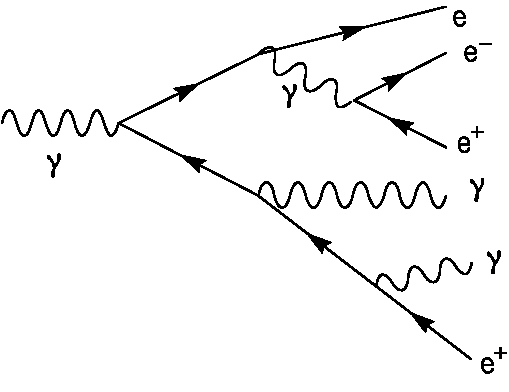
\includegraphics[scale=0.85]{Schematic_of_a_particle_shower.pdf}
  \caption{Esquema de una cascada electromagnética originada por un fotón.}
  \label{fig:cascada}
\end{figure}

Como se mencionó en la motivación física del problema, para detectar los neutrinos necesitamos detectar las cascadas producidas por los electrones. Según como se han definido las cascadas parece un problema difícil ya que en los detectores solo podemos ver a los electrones por lo que no podemos simplemente determinar qué partícula origina la cascada. Por lo tanto, si tuviésemos justo lo que acabamos de explicar resultaría prácticamente imposible distinguir las cascadas.

Sin embargo, sí existen diferencias entre las cascadas. La diferencia principal es que, para cascadas originadas por electrones al comienzo de la cascada se observa que el electrón recorre una distancia que podemos ver en el detector. Además, estos electrones que recorren una mayor distancia antes de desintegrarse también pueden tenerse en puntos posteriores de la cascada y son más probables para las cascadas originadas por electrones.

El hecho de saber la diferencia no hace que sea un proceso simple, en la Fig. \ref{} mostramos dos eventos del problema que vamos a estudiar en este trabajo donde vemos una cascada originada por un fotón y otra originada por un electrón. \red{Tengo que elegir las imágenes bien}

\subsection*{Detector LArTPC}


Como se ha mencionado, los datos con los que vamos a trabajar proceden de simulaciones realizadas sobre un detector LArTPC, que se empleará en programas como SBN y DUNE. Veamos detalladamente cómo funciona y cuál es la salida \cite{sbnd}. En la Fig. \ref{fig:sensado} se muestra el esquema de funcionamiento de este detector.

\begin{figure}[h!]
  \centering
  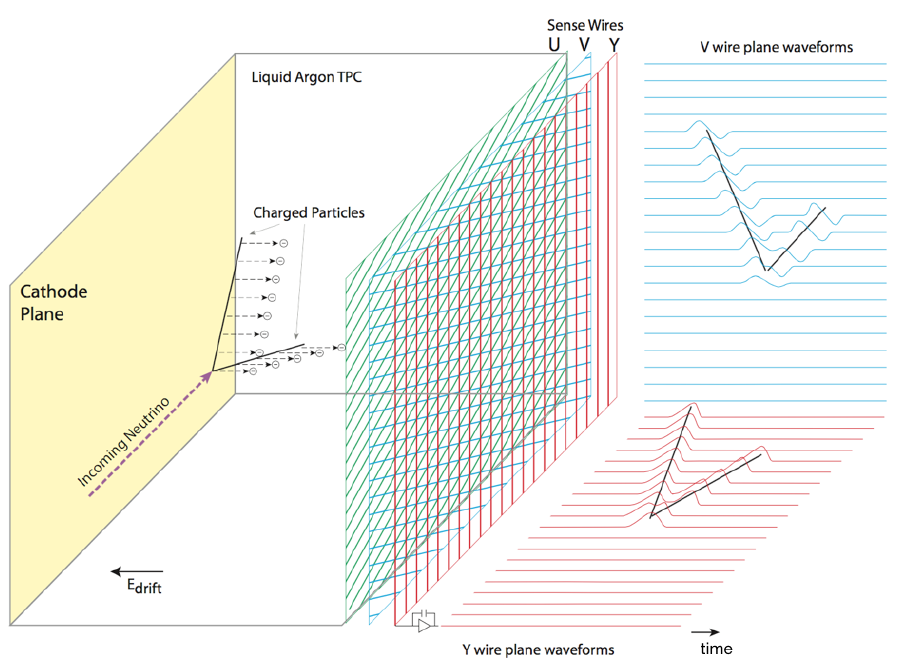
\includegraphics[scale=0.65]{planos_sensado.PNG}
  \caption{Esquema de funcionamiento de un TPC \cite{sbnd}. La partículas cargadas en el interior del detector arrancan electrones que son dirigidos hacia los planos de hilos donde se recogen su energía, posición en dicho plano y tiempo de llegada. Con esta información junto con el instante de tiempo inicial del evento se reconstruye la trayectoria de las partículas cargadas.}
  \label{fig:sensado}
\end{figure}

Estos detectores consisten en argón líquido (LAr) donde tiene lugar las interacciones y una cámara de proyección temporal (TPC) que nos permite trazar la trayectoria de partículas cargadas. El hecho que se use argón líquido es debido a que es un gas noble y por tanto es un gas inerte \red{que nos permite mantener el medio lo más puro posible}. Además, el Ar pose un potencial de ionización bajo de manera que es sencillo que una partícula cargada ionice el medio dejando electrones libre en el medio. A todo esto el Ar es el gas noble más abundante \cite{lar_review} lo que lo hace más accesible. 


El detector consiste en un criostato, dispositivo que nos permite mantener bajas temperaturas, que contiene el argón y está dividido en dos partes por un plano que va actuar como cátodo. Paralelo a este plano, en los extremos del criostato, vamos a tener planos de hilos que nos permiten registrar la señal dejada por un electrón (Fig. \ref{fig:estructura_detector}). Cada plano consiste en tres planos de cables y son el ánodo del circuito que van a recorre los electrones libres. Estos detectores nos permiten trazar la trayectoria de partículas cargadas que se desplacen en su interior.

En la Fig. \ref{fig:estructura_detector} mostramos un esquema de la estructura del detector, donde vamos a tomar como eje $x$ la dirección del campo eléctrico, es la dirección en la que se van a desplazar los electrones libres y se denomina dirección de deriva. Como eje $z$, se considera el lado más largo del volumen del detector y esta sera la dirección por donde entran los neutrinos. Finalmente, como eje $y$ tomaremos la dirección restante. Los planos de hilos se encuentran en los extremos del volumen en el plano YZ.

\begin{figure}[h!]
  \centering
  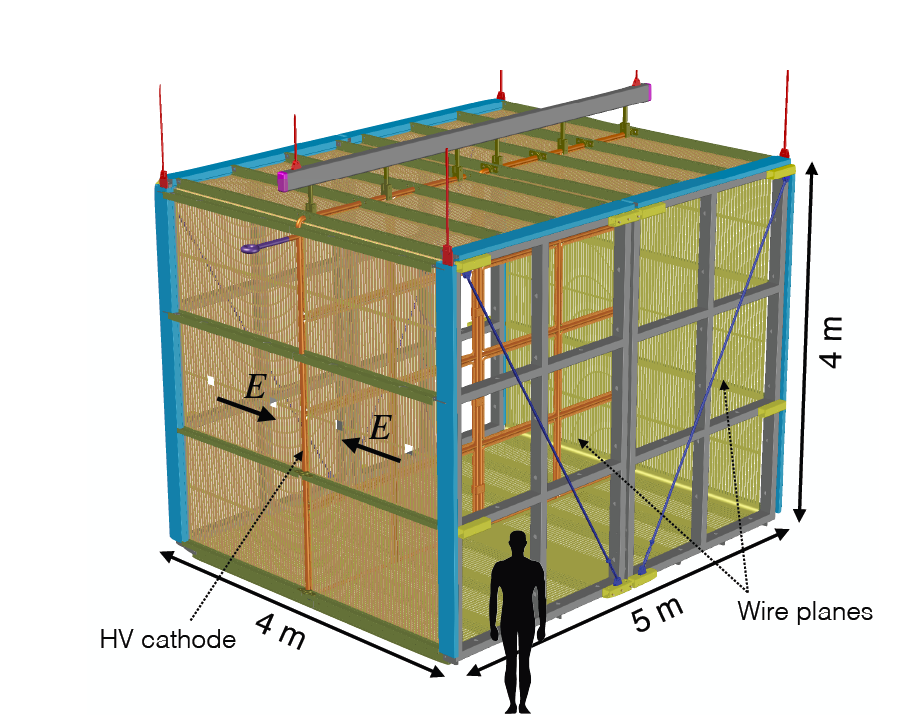
\includegraphics[scale=0.45]{estructura_detector.PNG}
  \caption{Esquema de la estructura del detector LArTPC del programa SNB \cite{sbnd}. En el eje $x$, la dirección de deriva, se observa el campo eléctrico aplicado para dirigir los electrones libres hacia los planos de hilos. El eje $z$ es el que contiene el lado más largo del detector y es la dirección con la que inciden los neutrinos. El eje $y$ es el eje restante. Vemos que perpendicular a la dirección de deriva tenemos un plano que parte el detector en dos regiones y actúa como cátodo. En los extremos se tienen los planos hilos que actúan como ánodos.}
  \label{fig:estructura_detector}
\end{figure}

Lo primero que vamos a mostrar es cómo dada una partícula cargada vamos a poder trazar su trayectoria. Para esto, tenemos que entender que cuando una partícula cargada se mueve por un medio neutro, si tiene energía suficiente, puede darse que por fuerza coulombiana se arranquen los electrones ligados al Ar teniendo electrones libres. De forma que al moverse una partícula cargada por un medio neutro lo que vamos a tener es una traza de electrones libres. En la Fig. \ref{fig:sensado} se puede ver representado gráficamente esto.

Al aplicar un campo eléctrico, los electrones libres son dirigidos hacía los planos de hilos que al llegar al plano son recogidos emitiendo un pulso eléctrico. Hay muchos detectores que usan este principio, como puede ser un contador Geiger. Sin embargo, con el LArTPC se pretende es reconstruir la trayectoria seguida por las partículas y para ello lo que se hace es lo siguiente. Por un lado, se usan fotodetectores para determinar el instante tiempo $t_0$ en el comienza la trayectoria. Este punto es el lugar donde el neutrino interacciona con el medio y por tanto el tiempo en el que comienza la trayectoria de las partículas que queremos estudiar. 


Cuando se origina la partícula cargada, esta se desplaza arrancando electrones que, con un campo eléctrico perpendicular al plano YX, dirigimos hasta los planos de hilos en los extremos. Cada plano de hilos consiste en tres planos de cables que se pueden observar en la Fig. \ref{fig:sensado}, donde en cada plano de cables, estos cables son paralelos y los tres planos tienen orientaciones distintas. La clave es que con dos de estos planos podemos determinar la posición  del electrón libre en dicho plano.


Para entender esto, simplifiquemos el problema. Supongamos que tenemos solo dos planos de hilos, uno vertical y otro horizontal, de manera que son perpendiculares entre sí, es decir tenemos una rejilla. Cuando llegue uno de los electrones libres al plano se producirá una pulso eléctrico en uno de los cables del plano vertical y en uno del horizontal por lo que sabiendo la posición de estos cables podemos determinar la posición del electrón arrancando en dicho plano. A estos pulsos les denominamos \textit{hits} y también recogemos información de la energía del electrón, ya que en el cable se recogerá una carga, proporcional a la energía, que es lo que se denomina carga del \textit{hit}. Además también sabremos cuándo llegan estos electrones al plano.

La situación real es que los planos no son horizontales y verticales y el tercer plano está para deshacer ambigüedades que se pueden dar al realizar la reconstrucción. De forma que, con los planos de hilos vamos a obtener la posición en el plano YZ de los electrones que hayan sido arrancados por la partícula cargada. Lo que es lo mismo, obtenemos la trayectoria de dicha partícula proyectada en el plano YZ. Para obtener información de la dimensión restante lo que hacemos es usar $t_0$ y el tiempo de llegada de los electrones al plano, ya que al saber la velocidad de deriva del electrón en el medio, podemos obtener la distancia al plano YZ.

En resumen, inicialmente llega un neutrino, que interacciona con el Ar, obteniendo un protón y un electrón (recordar que esta es una de las opciones posibles). Con los fotodetectores obtenemos el instante en el que tiene lugar esta interacción. Al ser ambas partículas cargadas, vamos a tener un rastro de electrones libres por cada partícula, que debido al campo eléctrico en el eje $x$ se desplazan hacía el plano de hilos. Obteniendo la posición de los electrones libres en el plano YZ y, de esta forma, tenemos la proyección de las trayectorias en dicho plano. La información de la trayectoria en el eje $x$ la obtenemos usando el tiempo de origen así como el tiempo en el que llegan los electrones al plano de hilos.

En definitiva, vamos a poder obtener la trayectoria completa de una partícula cargada ya que trazamos la trayectoria en distintos momentos gracias a los electrones arrancados. La forma de los datos una vez procesados se asemejan mucho a una imagen, ya que tendremos las coordenadas de los puntos de la trayectoria. Una analogía a las imágenes que vamos a usar es la estela dejada por un avión en el cielo marcando su trayectoria.

Nosotros vamos a centrarnos en el estudio de las cascadas electromagnéticas que se van a producir en el interior del detector. Una de las situaciones que podemos tener es que el neutrino llegue, produzca un electrón y un protón, este electrón va a desplazarse por el medio creando electrones libres (y por tanto lo observamos) hasta que se desintegré generando un electrón y un fotón iniciándose la cascada electromagnética. La otro opción posible, es que un fotón origine la cascada. Nuestro objetivo fundamental en este trabajo es conseguir distinguir ambos tipos de sucesos.

\subsubsection*{MLOps}

Un problema de ciencia de datos, es un proceso que puede llegar a ser muy complejo y depender de varias partes e incluso de varios equipos. Por ejemplo, primero tenemos que procesar los datos, analizarlos y entrenar un modelo. Una vez obtenido el modelo, este tiene que ponerse en funcionamiento y realizar la tarea para la que ha sido entrenado. En el momento que el proyecto crece, cada una de estas partes crece llegando a un punto en el que cualquier modificación que se quiera realizar puede ralentizarse mucho debido a la complejidad del sistema.

DevOps es un conjunto de prácticas para hacer el ciclo de desarrollo, implementación y ejecución de aplicaciones de forma eficiente \cite{mlops_nvidea}. MLOps, no es más que la aplicación de estas prácticas en una aplicación de Machine Learing. La filosofía de estos métodos de desarrollo es que los ciclos de versiones sean los más rápidos posibles con la idea de aprender del funcionamiento de la aplicación y de la opinión de los usuarios.

Si entrar en mucho detalle, veamos algunas de estas prácticas. El primer paso suele ser la integración y entrega continua que consiste en probar de forma automática el software introducido así como diseñar entorno a estas pruebas. Por otro lado, también se busca que el despliegue se realice de manera automática \cite{mlops_practical}. El empleo de sistemas de control de versiones como git es fundamental, al permitir tener un seguimiento de la evolución del proyecto así como la colaboración entre personas. 

En MLOps además se tiene que integrar integrar la parte de ciencia de datos donde tenemos por un lado el procesamiento de estos datos y por otro lado se tiene el modelo final que es lo que nos interesa monitorizar y mejorar. Con estas técnicas se pretende automatizar el tratamiento de los datos así como el despliegue y control sobre el modelo. En la Fig. \ref{fig:mlops} se muestra un esquema de un flujo de trabajo basado en MLOps donde tenemos primero la parte de ciencia de datos donde tenemos los datos y el modelo. Luego se tiene la parte de desarrollo donde de manera automática se verifica que todo funcione y se despliega. Tras el despliegue, entra en juego la parte de operaciones donde se hace uso de la aplicación y se aprende de su funcionamiento. Con esta información se modifican las etapas anteriores.

\begin{figure}[h!]
  \centering
  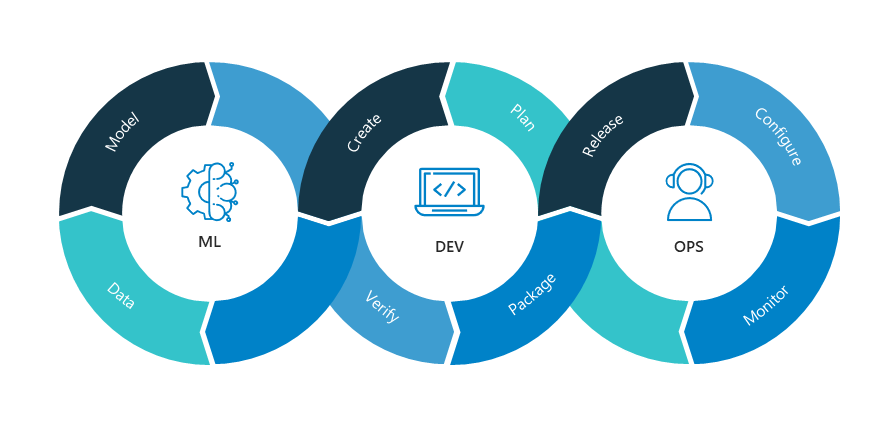
\includegraphics[scale=0.50]{mlops.PNG}
  \caption{Esquema del flujo de trabajo basado en MLOps \cite{mlops_neal}. En el centro tenemos el flujo de desarrollo donde tenemos primero la planificación y la creación de la aplicación. Luego, entramos en el flujo de ML donde se procesan los datos y se crea el modelo. Con esto volvemos al flujo de desarrollo donde se verifica y despliega la aplicación. Finalmente entra en juego el flujo de operación donde se monitoriza el modelo y la aplicación para que en función de su funcionamiento se vuelva a comenzar el ciclo.}
  \label{fig:mlops}
\end{figure}

Nosotros con este trabajo nos vamos a centrar sobre todo en implementar muy bien la estructura de automatización de los datos y modelos ya que nos va a permitir trabajar de manera mucho más ordenada y mantener un control de trabajo que vayamos realizando y de los modelos obtenidos. En \cite{mlops_begin} se muestran tres niveles de implementación de MLOps: un primero donde todo se hace de manera manual, un segundo donde hay una estructura de flujo donde con el uso de tuberías se automatizan la mayoría de elementos y un tercero donde se introduce la integración continua con el uso de test automatizados y el código se empaqueta y despliega automáticamente. Nosotros nos vamos a quedar en el segundo nivel donde tenemos un proceso completamente automático en el flujo de datos y del modelo pero no vamos a entrar en el uso de test automáticos así como en el despliegue automático del código al ser un proceso complejo, sobre todo para alguien sin experiencia previa, y alejarnos mucho del objetivo final de este trabajo. 

\subsection{Deep Learning}
\label{sec:dl}

El Deep Learning (DP) es un conjunto de técnicas y modelos que están dentro del ámbito del Machine Learning (ML) y que en los últimos años a experimentado unos enormes avances en muchos problemas de ciencia de datos que se habían resistido a los métodos clásicos \cite{dl_nature}. Entre estos problemas se encuentran la clasificación de imágenes, donde el uso de redes neuronales convolucionales (CNN) se han convertido en el estado del arte y han conseguido obtener mejores resultados que los propios humanos. Otros ejemplos se tiene en el procesamiento de lenguaje natural con los transformers o en el reconocimiento del habla \cite{korean_dl}.

El DL tiene la ventaja de que es capaz de trabajar con los datos en bruto, de hecho se definen como aquellos modelos que son capaces de obtener las características directamente de los datos \cite{dl_book}. Estos rápidos avances se deben en gran medida a que se disponen de una gran cantidad de datos (gracias al desarrollo del Big Data) que pueden ser procesados automáticamente así como de distintos avances tecnológicos \cite{korean_dl,dl_nature}. De hecho, los avances son tales que hemos pasado de ser capaces de ser capaces de realizar clasificación de imágenes a generar imágenes nuevas dados un texto donde se combinan distintos modelos de DL \cite{hier} o modelos que son capaces de escribir código dadas las instrucciones de lo que se quiere realizar \cite{codex}.

Con todo esto veamos los fundamentos necesarios para entender que es una CNN, sus elementos, su complejidad y mostraremos algunos ejemplos de esta arquitectura de red neuronal. No se entrará en mucho detalle pero en esta sección lo que se pretende es que entienda bien que es el DL y una CNN y cuales son los principios básicos. 

\subsubsection*{Fundamentos}

Las redes neuronales (NN) surgen con los perceptrones multicapa (MLP) que consisten en la composición de funciones paramétricas para formar una función más compleja. Este modelo está inspirado en el funcionamiento del cerebro, mediante las conexiones entre neurona y la activación de las mismas. Esta representación se puede observar en la Fig. \ref{fig:mlp} pero no es más que una representación de una serie de operaciones matemáticas, donde los nodos representan las entradas y salidas de funciones y los enlaces el valor de los coeficientes de la aplicación, que se denominan pesos. 
\begin{figure}[h!]
  \centering
  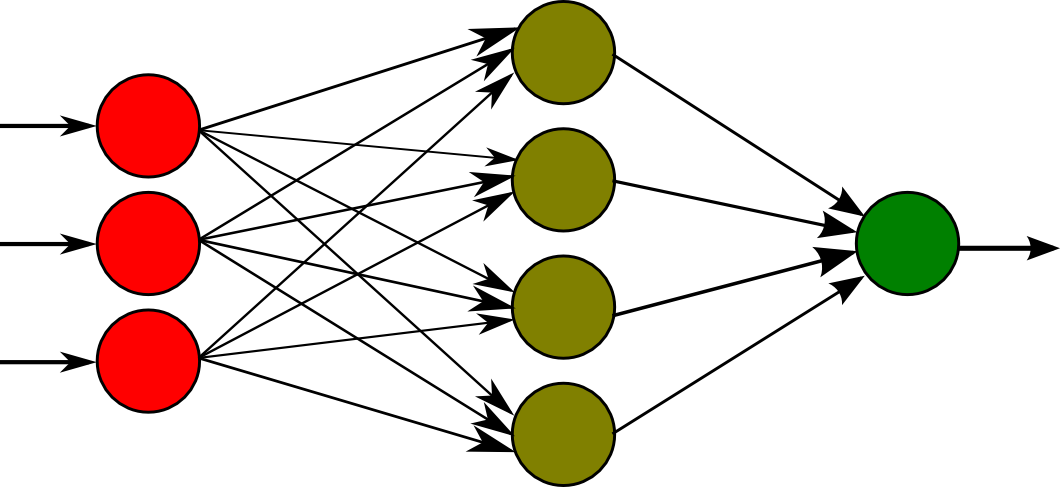
\includegraphics[scale=0.29]{MultiLayerPerceptron.png}
  \caption{Esquema de un modelo MLP con una capa de entrada, una capa oculta y una capa de salida \cite{mlp}.}
  \label{fig:mlp}
\end{figure}

De hecho el paso de una capa a otra en un MLP no es más que una aplicación lineal:
\begin{equation}
  \label{eq:mlp_1}
  \mathbf{y} = W\mathbf{x},
\end{equation}
a la que se le aplica una función no lineal. Donde $\mathbf{x} \in \mathbb{R}^n $ es la entrada y son los nodos iniciales, $\mathbf{y} \in \mathbb{R}^m$ son los nodos de salida y la matriz $W$ se representa por los enlaces. Notar que las dimensiones de entrada y de salida no tienen por que ser las mismas. La función no lineal se aplica que el modelo sea capaz de aprender relaciones más complejas y hay muchas opciones normalmente se usa la sigmoide o la RELU entre otras muchas \cite{dl_book}.

En la ecuación \ref{eq:mlp_1} lo que hemos mostrado es la función matemática de una MLP donde solo tenemos una capa de entrada y otra de salida y donde no se aplica ninguna función no lineal, por lo que es un ejemplo que es idéntico a un modelo de regresión. Se puede añadir más complejidad añadiendo más capas y estas funciones no lineales. Un ejemplo de la formulación de una MPL con una capa oculta es:
\begin{equation}
  \mathbf{y} = \sigma(W\mathbf{x}), \quad \mathbf{z} = \sigma(V\mathbf{y}),
\end{equation}
donde $\sigma$ representa la función sigmoide, $\mathbf{x}$ es el vector de entrada, $\mathbf{y}$ es el de salida de la capa inicial y $\mathbf{z}$ el vector de salida. W y V son matrices que representan los enlaces entre capas.

Una cosa importante sobre estos modelos es que se puede demostrar que son aproximadores universales, es decir, que una toda función puede aproximarse usando una MLP, el problema surge con la cantidad de capas y neuronas necesarias así como en el proceso de aprendizaje de los pesos correctos para representar dicha función.

El punto más importante de los modelos de DL en general y lo que los define es que son capaces de aprender las características (variables) para resolver el problema. Hasta entonces, si se quería estudiar una imagen lo que se hacía era aplicar distintos algoritmos como LBP para obtener las características que nos permitan realizar una cierta tarea. El problema es que el diseño de estos algoritmos requiere de un esfuerzo muy grande y los resultados no son los mejores. Como ya hemos dicho, esto es posiblemente uno de factores que han hecho posible que se tengan grandes avances ya que no tenemos que perder tanto tiempo en la extracción de características \cite{dl_nature}. Estos modelos no solo agilizan el proceso, si no que además son capaces de detectar patrones que nosotros no.

Las MLP establece las bases de todos los modelos actuales de Deep Learning. Con el tiempo han ido surgiendo distintos tipos de NN como las CNN, las RNN, los autoencoder o los transformers. En las MLP el paso de una capa a otra no es más que la aplicar una función no lineal tras realizar una aplicación lineal sobre un vector de entrada. Estas nuevas arquitecturas lo que hacen es cambiar esta representación y por tanto cambiando la función realizada. Como se definan las redes influirá en los tipos de datos con los que la red podrá trabajar. 

Un aspecto importante es que si nos fijamos, las NN, por definición, no son más que la composición de distintas funciones donde cada función la podemos entender como una capa o incluso un conjunto de capas (la composición de funciones es una función). Esto simplifica la construcción de redes en el sentido conceptual ya que simplemente hay que pensar en la combinación de distintos bloques. Por ejemplo, a las capas que forman una MLP se le denominan densas (todos los nodos están unidos) y un MLP no es más que el uso de varias de estas capas. En las CNN se usan lo que se denominan capas de convolución, que son un conjunto de capas que realizan la operación de convolución. Hay otros muchos bloques y el diseño de una NN consiste en la aplicación de sucesivos bloques que dependerán del objetivo final que se tenga.

La dificultad reside en construir bloques que sirvan para el tipo de datos que se este usando y como combinar los bloques para obtener los resultados deseados pero nos en la construcción del modelo una vez sabemos cual es su forma.

\subsubsection*{CNN}

Las CNN son un tipo de NN donde la función matemática que se realiza es la de convolución. Antes de entrar en la parte matemática, mostremos la idea detrás de esta capa de convolución. Para ello supongamos que tenemos una imagen, que se representa como una matriz donde cada elemento describe al píxel.

Sobre esta imagen podemos ir aplicando un filtro pequeño, i.e un bloque $3\times 3$ e ir recorriendo la imagen y recogiendo el resultado de aplicar el filtro. Entiéndase aplicar el filtro como sumar los píxeles de la imagen que pase por un patrón fijo, por ejemplo podría se una linea diagonal. Esto matemáticamente lo podemos ver como tenemos una matriz $I$, la imagen, y una $K$, el filtro, donde las dimensiones de $I$ son mayores que las de $K$. La matriz $K$ se fija definiendo el filtro (en el caso de tener la linea diagonal tendríamos nulo) y lo que se hace es ir recorriendo $I$ en bloques y hacer un producto elemento a elemento y sumarlo de manera que si recogemos todos los resultados en una matriz el resultado de aplicar el filtro sería otra matriz.

Sea $I$ una matriz de dimensiones $p\times q$ y $K$ una matriz de dimensiones $r\times s$ tal que $p>r$ y $q>s$. Definimos aplicar un filtro como:
\begin{equation}
  \label{ec:def_filtro}
  S_{i, j} = \sum_{n=1}^{r}\sum_{m=1}^{s}I_{i + n, j + m}K_{n,m}
\end{equation}
con $i\in\{1,\dots, p -1 \}$ y $j\in\{1,\dots, 1 -1\}$. La matriz $S$ tiene dimensiones $p-1\times q-1$. Sin entrar en mucho más detalle, hay distintas definiciones según como tratemos los bordes de la imagen, por ejemplo, podríamos considerar que cuando nos saliésemos de la imagen se vuelva al otro extremo de manera que la matriz resultante tendría las mismas dimensiones que la imagen original. Otra cosa que podemos notar es que en la definición solo se contempla que el filtro se aplique sobre todos los bloques posibles. Sin embargo, también se puede hacer de manera que el desplazamiento realizado al desplazar el filtro no sea un píxel.

Este enfoque nos permite determinar que regiones de la imagen tienen unos patrones que nos pueden interesar. Con las CNN lo que se consigue es que la forma de estos filtros son aprendidos por la red. 

Esta aplicación que acabamos de describir es lo que se denomina convolución. Matemáticamente la convolución entre dos funciones $(x * w)(t)$ se puede escribir, en el caso de una dimensión, como:
\begin{equation}
  (x * w)(t):=\int_{-\infty}^{\infty} x(a) w(t-a) d a,
\end{equation}
donde $x$ y $w$ son funciones que dependen de una variable. En el ámbito del DL a $x$ se le denomina entrada y a $w$ el kernel \cite{dl_book}. La expresión en el caso discreto:
\begin{equation}
  (x * w)(t)=\sum_{a=-\infty}^{\infty} x[a] w[t-a].
  \end{equation}
Esta definición se puede generalizar para varias dimensiones simplemente añadiendo tantas integrales como dimensiones. En el caso de las imágenes tenemos que el espacio es discreto y que tenemos dos dimensiones, entonces, la operación de convolución quedaría:
\begin{equation}
  s[i, j]=(I * K)[i, j]=\sum_{m} \sum_{n} I[m, n] K[i-m, j-n],
\end{equation}
donde $I$ es una matriz de dimensiones $p\times q$, la entrada, y $K$ es una matriz de dimensiones $k\times l$, el kernel. Los límites de los sumatorios realmente serían de menos infinito a infinito pero en nuestro caso está determinado por las dimensiones de K (podemos definir $K = 0$ si los indices superan las dimensiones). Notar la gran similitud con \ref{ec:def_filtro}.

% Veamos esta expresión con el ejemplo que pusimos antes. $I$ es una matriz dada por la imagen, $K$ es el filtro y $s$ es la matriz final tras aplicar el filtro. Notar que la ecuación esta definida para los elementos de las matrices. La expresión anterior lo que nos dice es que el elemento $i$, $j$ de la matriz $s$ esta dado por hacer el producto elemento a elemento de la matriz $K$ con una parte de la matriz $I$ en un entorno del elemento $i$, $j$. Tras hacer el producto lo que se hace es sumar. Esto lo hacemos para todos los $i$, $j$ posibles y es lo que antes decíamos de aplicar el filtro a la imagen.

La capa de convolución consiste en aplicar el filtro y luego (en la mayoría de casos) aplicar una capa de reducción \textit{pooling} que consiste en reducir las dimensiones de la salida mediante la agregación de un grupo de píxeles. Por ejemplo, una imagen la podemos reducir si fragmentamos la imagen en bloques $2\times 2$ y le hacemos la media a estos bloques. Esta operación ayuda a que el resultado de la aplicación del filtro sea invariante a pequeños desplazamientos, que es fundamental a la hora de estudiar imágenes ya que queremos que imágenes que se distingan solo por desplazamientos se clasifiquen igual (pensar que la imagen puede estar tomada desde puntos de vista distintos pero contener el mismo objeto).

Estos son los elementos básicos de una CNN y es el punto de partida a la hora de construirlas. En resumen, hay muchas arquitecturas posibles para un NN donde cada una tendrá unas características que hacen que sean útiles para un tipo de problema concreto. En concreto, las CNN son muy buenas para a la hora de estudiar imágenes ya que permiten estudiar regiones de la imagen y determinar que elementos y patrones se tienen en la imagen, desde patrones muy simples que se obtiene con las primeras capas de convolución a patrones más complejos cuando aumentamos la complejidad del modelo.

\subsubsection*{Aprendizaje}

Hasta ahora hemos hablado de como es una NN. Sin embargo, no hemos entrado en como se determinan los pesos para que sean capaces de resolver un problema determinado. Sin entrar en mucho detalle, lo que se hace es emplear lo que se conoce como el descenso del gradiente y la \textit{backpropagation}.

El objetivo de un problema de ciencia de datos es que dados unos datos usar un modelo que sea capaz de realizar una determinada tarea sobre estos datos con la intención de obtener patrones no triviales. En el caso del aprendizaje supervisado, se parte de que se tienen unos datos que sabemos su clase/valor y con estos datos se entrena el modelo para que realice la tarea concreta. Las NN lo que hacen es hacer uso de los datos y sus etiquetas para determinar los pesos que mejor realizan la tarea concreta que se este realizado. Como ejemplo de tarea tenemos la clasificación que consiste en dada una instancia determinar la clase de salida.

El descenso del gradiente consiste en definir una función perdida que toma la clase dada por la red y la compara con la clase real. En el caso que la red se equivoque la salida de la función perdida será mayor y será menor a medida que el modelo acierte la clase de las distintas instancias. Esta función va a depender de los pesos de la red ya que son estos pesos los que determinan la clase que se asigna a la instancia. El descenso del gradiente consiste en obtener el gradiente esta función perdida con respecto a los parámetros de la red obteniendo la dirección de crecimiento de la función. Lo que se hace es modificar los pesos en la dirección contraria con la idea de reducir el valor de la función perdida que implica obtener mejores resultados.

Matemáticamente hablando el problema consiste en la optimización de una función de varias variables, los pesos de red. Los pesos se inicializan de manera aleatoria y se modifican calculando el gradiente y cambiando estos pesos en función del valor obtenido. El cambio se hace poco a poco y se regula con lo que se conoce como ritmo de aprendizaje ($lr$). Hay distintos algoritmos para este problema como puede ser SGD o Adam.

El proceso de aprendizaje suele realizarse dando un pequeño conjunto de datos obteniendo el valor de la función perdida para cada dato, promediando y finalmente ajustar los pesos calculando el gradiente. Esto se repite para todos las instancias y, normalmente, este procedimiento se repite de manera que durante el aprendizaje el modelo estudia cada dato varias veces. A el conjunto de datos pequeños se le conoce como \textit{batch size} ($bs$) y al número de veces que se recorre el conjunto de datos como número de épocas ($n_e$).

Uno de los problemas fundamentales que se tienen con el DL es que a medida que se tienen redes complejas el número de pesos aumenta y esto hace que sea relativamente simple tener sobre ajuste. De hecho una de las limitaciones del DL es la gran cantidad de datos que se necesitan para entrenar los modelos. Este problema ha hecho que hayan surgido métodos de regulación como el dropout que tratan de lidiar con este problema. El dropout no es más que eliminar aleatoriamente un porcentaje de los enlaces entre dos capas que a mostrado buenos resultados para lidiar con este problema.

Otras alternativas para reducir el sobre ajuste consisten en introducir pequeñas modificaciones sobre la imágenes para aumentar la variabilidad de los datos así como la cantidad de imágenes. Estas transformaciones suelen ser rotaciones, desplazamientos, cambios de brillo, reflexiones, etc. Esto es lo que se conoce como \textit{data augmentation} y ha mostrado dar muy buenos resultados \cite{dataaug}. Sin embargo, no vamos a hacer uso de esta técnica, ya que trabajamos con simulaciones y podemos hasta cierto punto obtener más datos en caso que sea necesario y porque transformaciones como rotaciones y reflexiones modifican la geometría del detector que es algo no deseado.

Otra opción es hacer uso de modelos ya entrenados con conjuntos de datos con muchas imágenes y muchas clases. La idea de tras de este enfoque consiste en que estas redes han aprendido muchos patrones que se pueden aplicar en otras situaciones. Se puede usar la red completa o únicamente el extractor de características. El aprendizaje consiste en entrenar el clasificador (en el caso de usar la red completa sería únicamente la capa) o modificar los pesos de las capas más profundas al ser la capas que contienen los patrones más complejos y por tanto pueden ser más específicos y por tanto no ser buenos para otro problema.

\subsubsection*{Elementos}

A modo de resumen final, vamos a recoger lo distintos bloques que pueden formar una CNN.

Un elemento necesario es el optimizador, el algoritmo que realiza el descenso del gradiente, y el $lr$. En este punto lo que se hace es construir la NN usando distintas capas. Las capas más simples son las que hemos ido mencionado. Se tiene el bloque de convolución que esta formado por la aplicación de los filtros así como de la capa de pooling. El otro elemento que hemos visto son las capas densas. Una CNN muy simple la podemos construir como la aplicación de varias capas de convolución y tras esto usar una MLP que clasifique los resultados.

Esto son los bloques más simples pero con el tiempo han ido surgiendo nuevos bloques y modificaciones sobre estos con la idea de mejorar la optimización o los resultados. También hay distintas forma de unir todos estos elementos para construir la red. No vamos a entrar en estos bloques ya que los avances en los últimos años a sido muy grande y una revisión de estos elementos es un trabajo en si. En el caso de hacer uso de alguna de estas arquitecturas o elementos lo describiremos cuando se describa dicha arquitectura.

\subsection{Estado del arte}

En los últimos años distintos laboratorios como el CERN han aplicado técnicas de DL \cite{ml_phy} con la idea de mejorar la capacidad de análisis de los datos que se obtienen. Algunas de la aplicaciones que se pueden encontrar son en seguimiento de partículas, identificación de eventos, identificación de \textit{Jets} o simulaciones aplicando redes generativas \cite{dl_phy, dl_lhc}. De hecho en microBooNE, un detector similar al nuestro, hace uso de las CNN para la clasificación de las cascadas \cite{ml_phy}.

Los neutrinos estériles surgen como una explicación teórica fuera del Modelo Estándar de una serie de resultados anómalos en distintos detectores de neutrinos. En los detectores LSND \cite{lsnd}, MiniBooNE \cite{miniboo} se han observado exceso del número de neutrinos esperados y que son compatibles con la existencia del cuarto neutrino \cite{sbnd}. Además se han observado otras anomalías conocidas como la anomalía del reactor o la anomalía de Galio que también podrían explicarse con la presencia del neutrino estéril. Los programas SNB y DUNE tiene como objetivo realizar experimentos de seguimiento que traten de confirmar que efectivamente se tienen esas anomalías \cite{sbnd, dune}. El detector microBooNE \cite{microboo} tenía un objetivo similar y ha publicado resultados recientemente, que son inconsistentes con los resultados de MiniBooNE  \cite{micro_res}. Sin embargo, no dejan de ser unos resultados iniciales y siguen teniendo incertidumbres tales que no descartan completamente los resultados previos. Una de las incertidumbres principales proviene de la selección de los eventos que provienen de neutrinos y por tanto para reducir la incertidumbre una de las cosas que hay que mejorar es la detección de cascadas electromagnéticas. 

Con respecto a la clasificación de imágenes, los mejores resultados en los últimos años vienen dados por CNN con arquitecturas cada vez más complejas y más profundas. El rendimiento de estos modelos se suele evaluar en una competición anual con el conjunto de datos de ImageNet, que tiene muchas imágenes con muchas clases. Los ganadores de de los últimos años han sido redes basadas en EfficientNet \cite{efficientnet}, que lo que hacen es introducir formas de escalar las redes (aumentar el número de capas y número de filtros) partiendo de un modelo base. Sin embargo, en los dos últimos años los ganadores no han sido modelos basados en CNN si no modelos que hacen uso de los transformers \cite{transformers} que son una nueva arquitectura de NN que han se han convertido en el estado del arte en procesamiento de lenguaje natural. Los modelos que aplican los transformers a la clasificación de imágenes se conocen como Visual Transformers (ViT) \cite{vit}, donde lo que hacen es proponer una forma de tratar las imágenes para que pueden ser usados por los transformers. Lo que proponen es segmentar la imagen en bloques ($16\times 16$) y, manteniendo un orden, se pasan estos bloques a la red como si fueran una frase.





\section{Clasificación de cascadas electromagnética}

% \red{En este punto se asume que se entiende que es una cascada, como funciona el detector y por tanto que trabajamos con algo muy parecido a imágenes. También se asume que se sabe a que nos referimos con hit. Realmente todo el aspecto físico debe estar explicado ene este punto}

En esta sección se muestra como vamos a abordar el problema propuesto. Para ello, primero describiremos cuál es el problema y cuáles son los datos con los que partimos. Luego, mostraremos las formas que hemos planteado para resolver el problema tanto en los modelos como en el procesamiento de los datos.

En ningún vamos a entrar en ningún momento en el código empleado más allá de un esquema del flujo que hemos empleado. Gran parte de este trabajo a consistido en la implementación del flujo completo ya que se ha partido desde cero. Además se ha dedicado una especial atención a realizar una implementación tratando de aplicar buenas prácticas de programación \cite{clean} así como mantener una estructura de MLOps, teniendo en cuenta que como físico no se tenía una formación previa de como abordar de manera correcta un proyecto de desarrollo software. Si bien es cierto que estas prácticas no son necesarias como tal, son muy buenas prácticas tanto como formación personal como para la realización de un proyecto que es posible que otras personas puedan continuar en un futuro.

Ahora vamos a hacer una descripción del problema que vamos a tener que resolver, así como de los datos proporcionados. También se mostrarán los distintos enfoques que se pueden plantear para la resolución del problema junto con los modelos que se pueden emplear para realizar la clasificación.
\subsection{Descripción del problema}

Como ya se ha mencionado, nuestro problema consiste en la clasificación de un tipo de evento que puede darse en un detector LArTPC, este evento se conoce como cascada electromagnética y puede originarse por un electrón o por un fotón. Nuestro objetivo es conseguir saber si una cascada es de origen fotónico o electrónico. En la Sección \ref{sec:conceptos} se ha descrito de manera detallada cómo se producen dichas cascadas y cómo el detector transforma pulsos eléctricos en los datos con los que nosotros vamos a trabajar.

En nuestro caso los datos están simplificados para contener únicamente cascadas electromagnéticas, por lo tanto, estos eventos son las trayectorias dejadas por las cascadas electromagnéticas observadas por el detector. Estos eventos los tenemos clasificados en función de que tipo de partícula origina el evento.

% Lo primero que tenemos que entender es que para cada cascada vamos a tener muchos datos que nos van a permitir reconstruir tridimensionalmente la cascada. A cada una de las cascadas nos referiremos como eventos. Para cada uno de los eventos sabremos cual es la partícula que lo origina así como la energía de dicha partícula. Para la reconstrucción tenemos la posición tridimensional de donde se produce el \red{hit} y la carga depositada por dicho \red{hit}. 

Los datos que se nos han proporcionado consisten en datos tabulares etiquetados por el tipo de cascada. Tenemos 7 columnas, tres de ellas hacen referencia a un identificador del evento, a su energía en GeV\footnote{Un eV se define como la energía que tiene un electrón al aplicarle un campo eléctrico con una diferencia de potencial de 1V.} y al tipo de partícula respectivamente\footnote{El Particle Data Group, con la idea de tener un identificador único y estandarizado para todas las partículas, asignó un número natural a cada única de las partículas para su identificación \cite{datagroup}. Las partículas que pueden originar los eventos que estamos estudiando son un electrón y el fotón cuyos identificadores son el 11 y 22 respectivamente.}.  También se tienen otras tres columnas que describen la posición tridimensional del hit dando las coordenadas $x$, $y$, $z$. La última recoge la cantidad de carga recogida del hit, por lo que es una magnitud proporcional a la energía depositada por la partícula cargada en ese punto de la trayectoria \red{unidades}. Es importante notar que en los datos no tenemos una única fila por evento, para cada evento tenemos varias filas con las que se describen la trayectoria completa del mismo.

Los datos con los que trabajamos provienen de simulaciones de Montecarlo que simulan con mucha exactitud el comportamiento real del detector. El uso de simulaciones supone una serie de ventajas. Por un lado, tenemos una gran cantidad de datos y en caso de ser necesario un mayor volumen de datos podría conseguirse hasta cierto punto. Por otro lado, al tener control total de la simulación sabemos información privilegiada en el sentido de que es información que no se tiene en el detector real y se tiene que inferir. En concreto tenemos el valor de la energía del evento, que realmente se tiene que inferir de las medidas. Por esto mismo, a la hora de hacer la clasificación no vamos a hacer uso de esta variable pero si la usaremos para validar el modelo y saber así si nuestro modelo es mejor para un intervalo de energía concreto.

Como hemos dicho los datos que tenemos están simplificados de manera que los eventos sean únicamente cascadas electromagnéticas. Realmente en cada evento tenemos distintas trayectorias dejadas por distintas partículas. Por lo que en la realidad sería necesario aplicar detección de objetos y quedarnos únicamente con las cascadas, sin embargo, para esto necesitamos un buen clasificador que es que abordamos aquí. En este trabajo no vamos a realizar la detección de objetos. 

Los eventos con los que vamos a trabajar siguen una distribución uniforme en energía y en la Fig. \ref{fig:3d} se muestran una representación tridimensional de los datos tal cual se nos han proporcionado así como las tres vistas del evento en la Fig. \ref{fig:vistas}. \red{TODO: poner gráficas bonitas tamaño de letra y evento más bonito. recortar la imagen.}

\begin{figure}[h!]
  \centering
  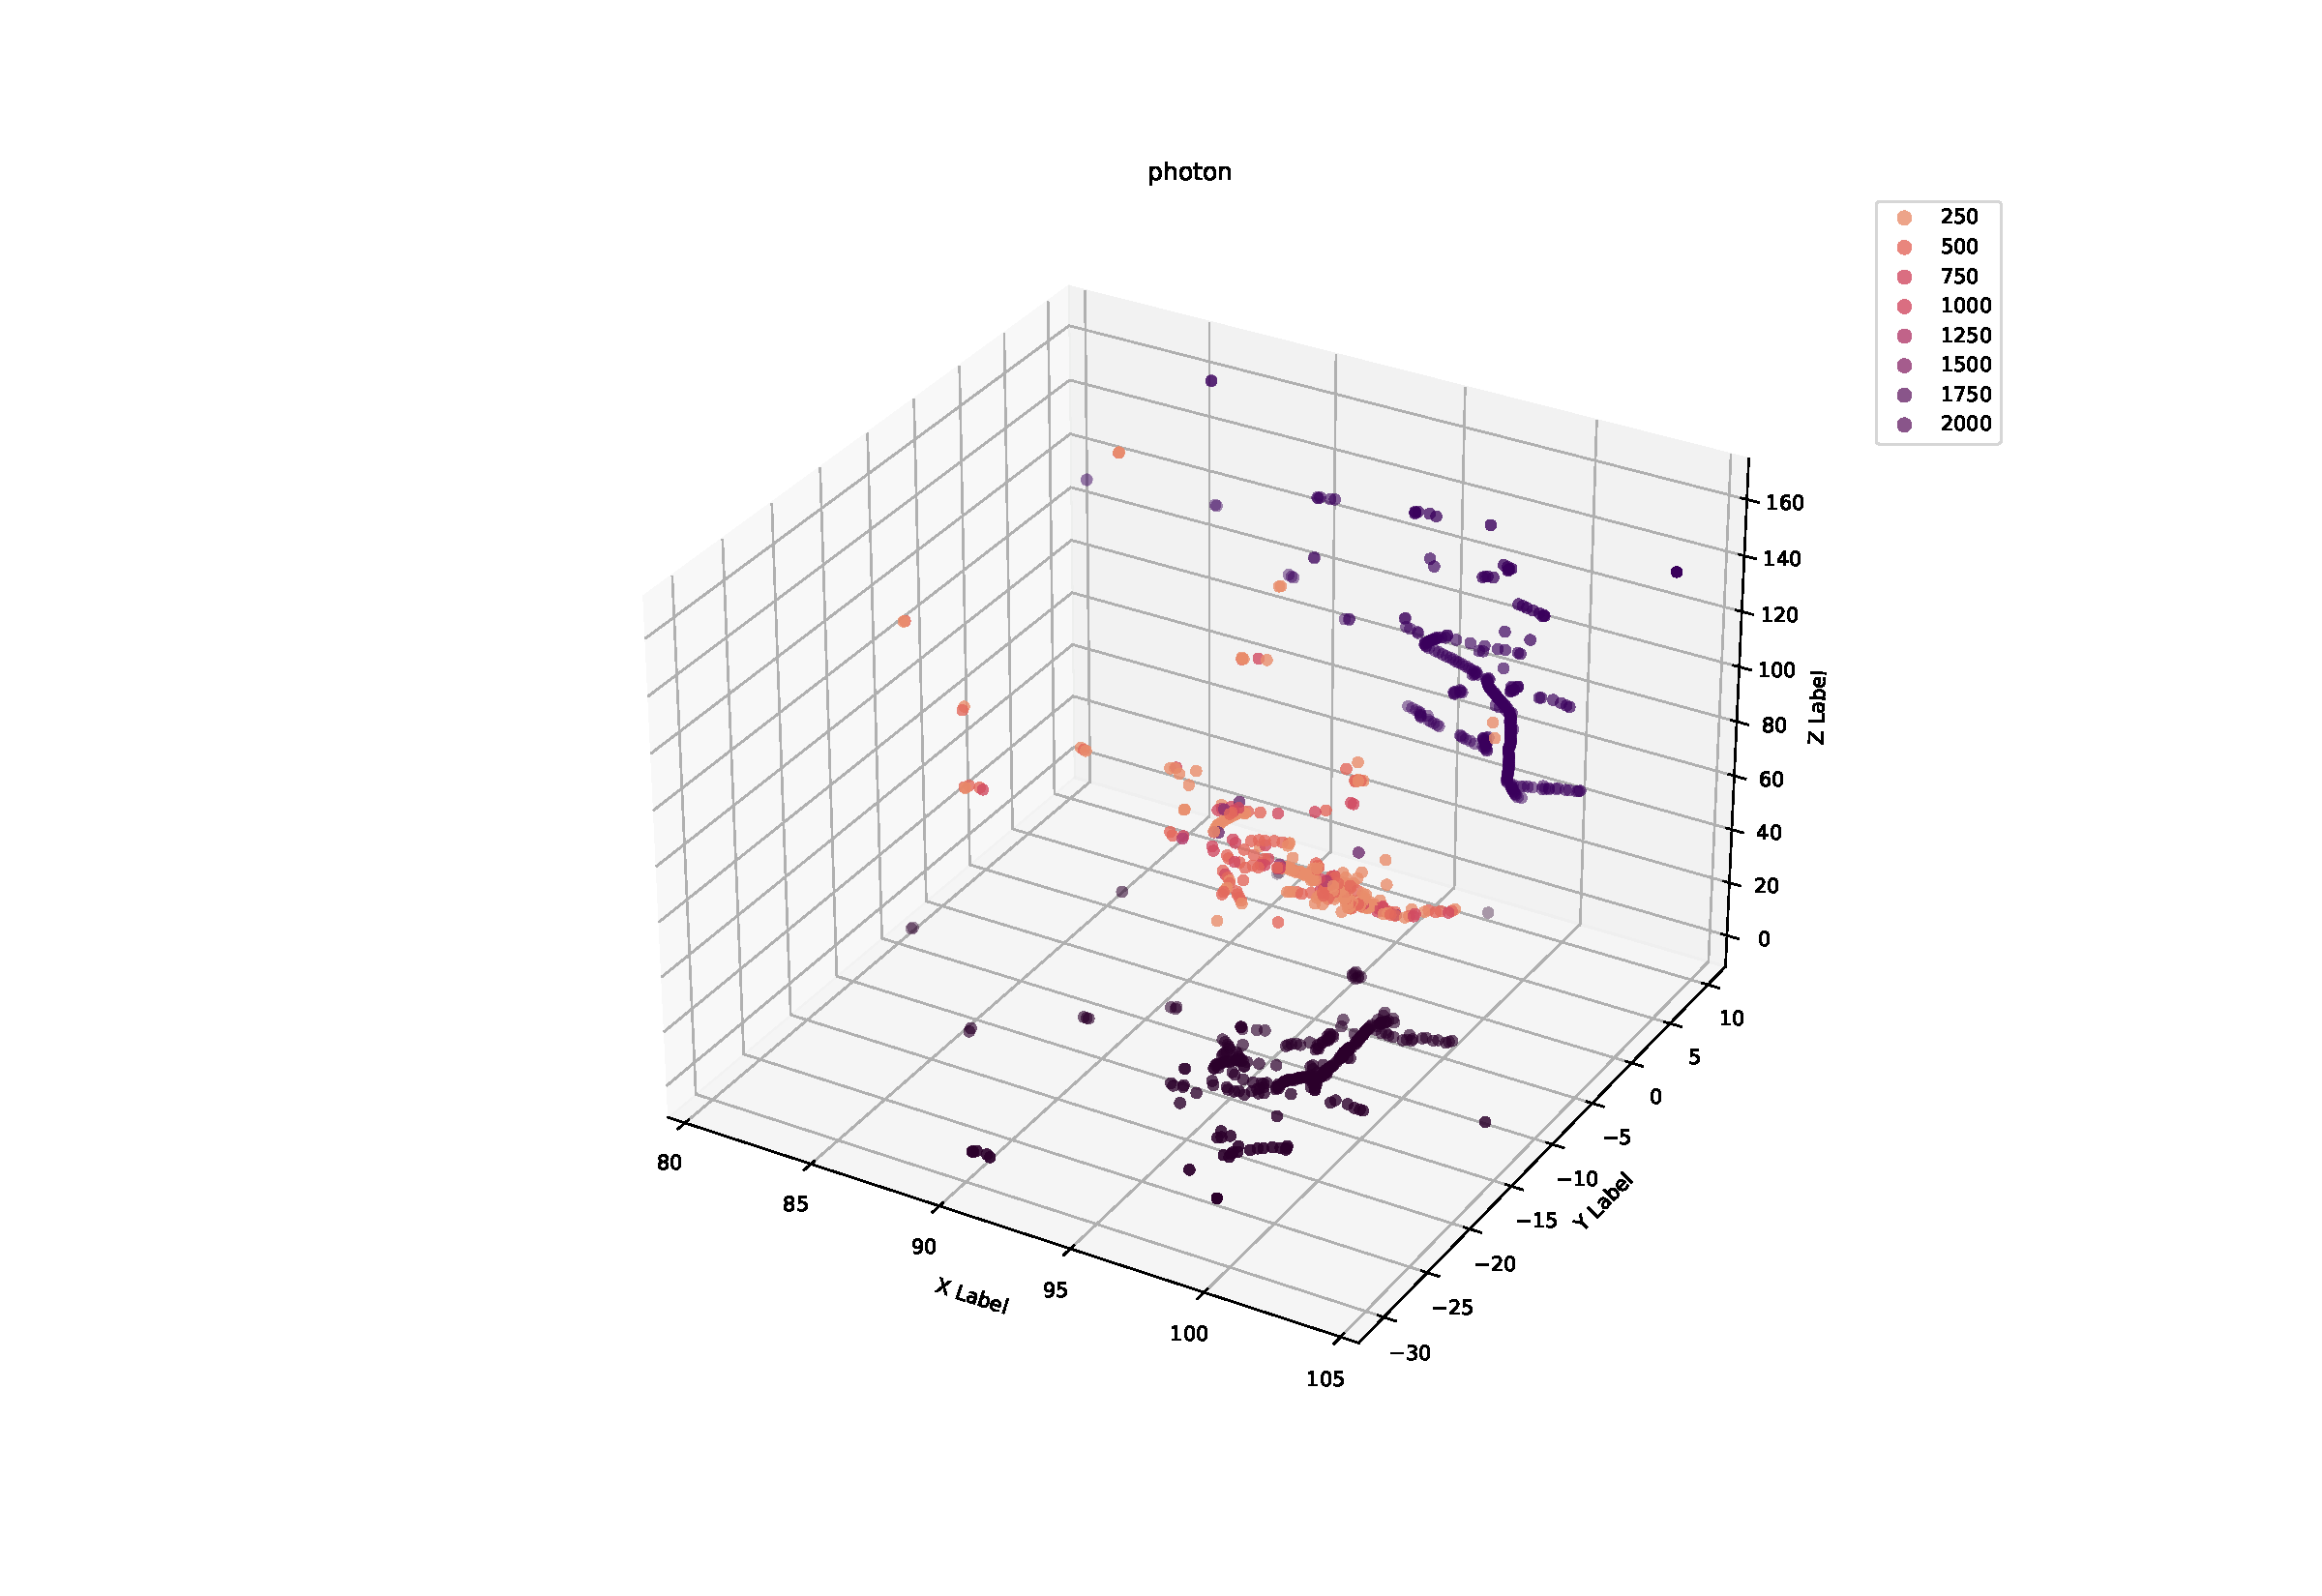
\includegraphics[scale=0.39]{3d_3.pdf}
  \caption{Representación tridimensional de una cascada electromagnética originada por un fotón con los datos en bruto. El color de los puntos viene dado en función de la carga del \textit{hit}. Se muestran también las proyecciones sobre el plano XZ y sobre el plano XY con colores fijos.}
  \label{fig:3d}
\end{figure}
\begin{figure}[h!]
  \centering
  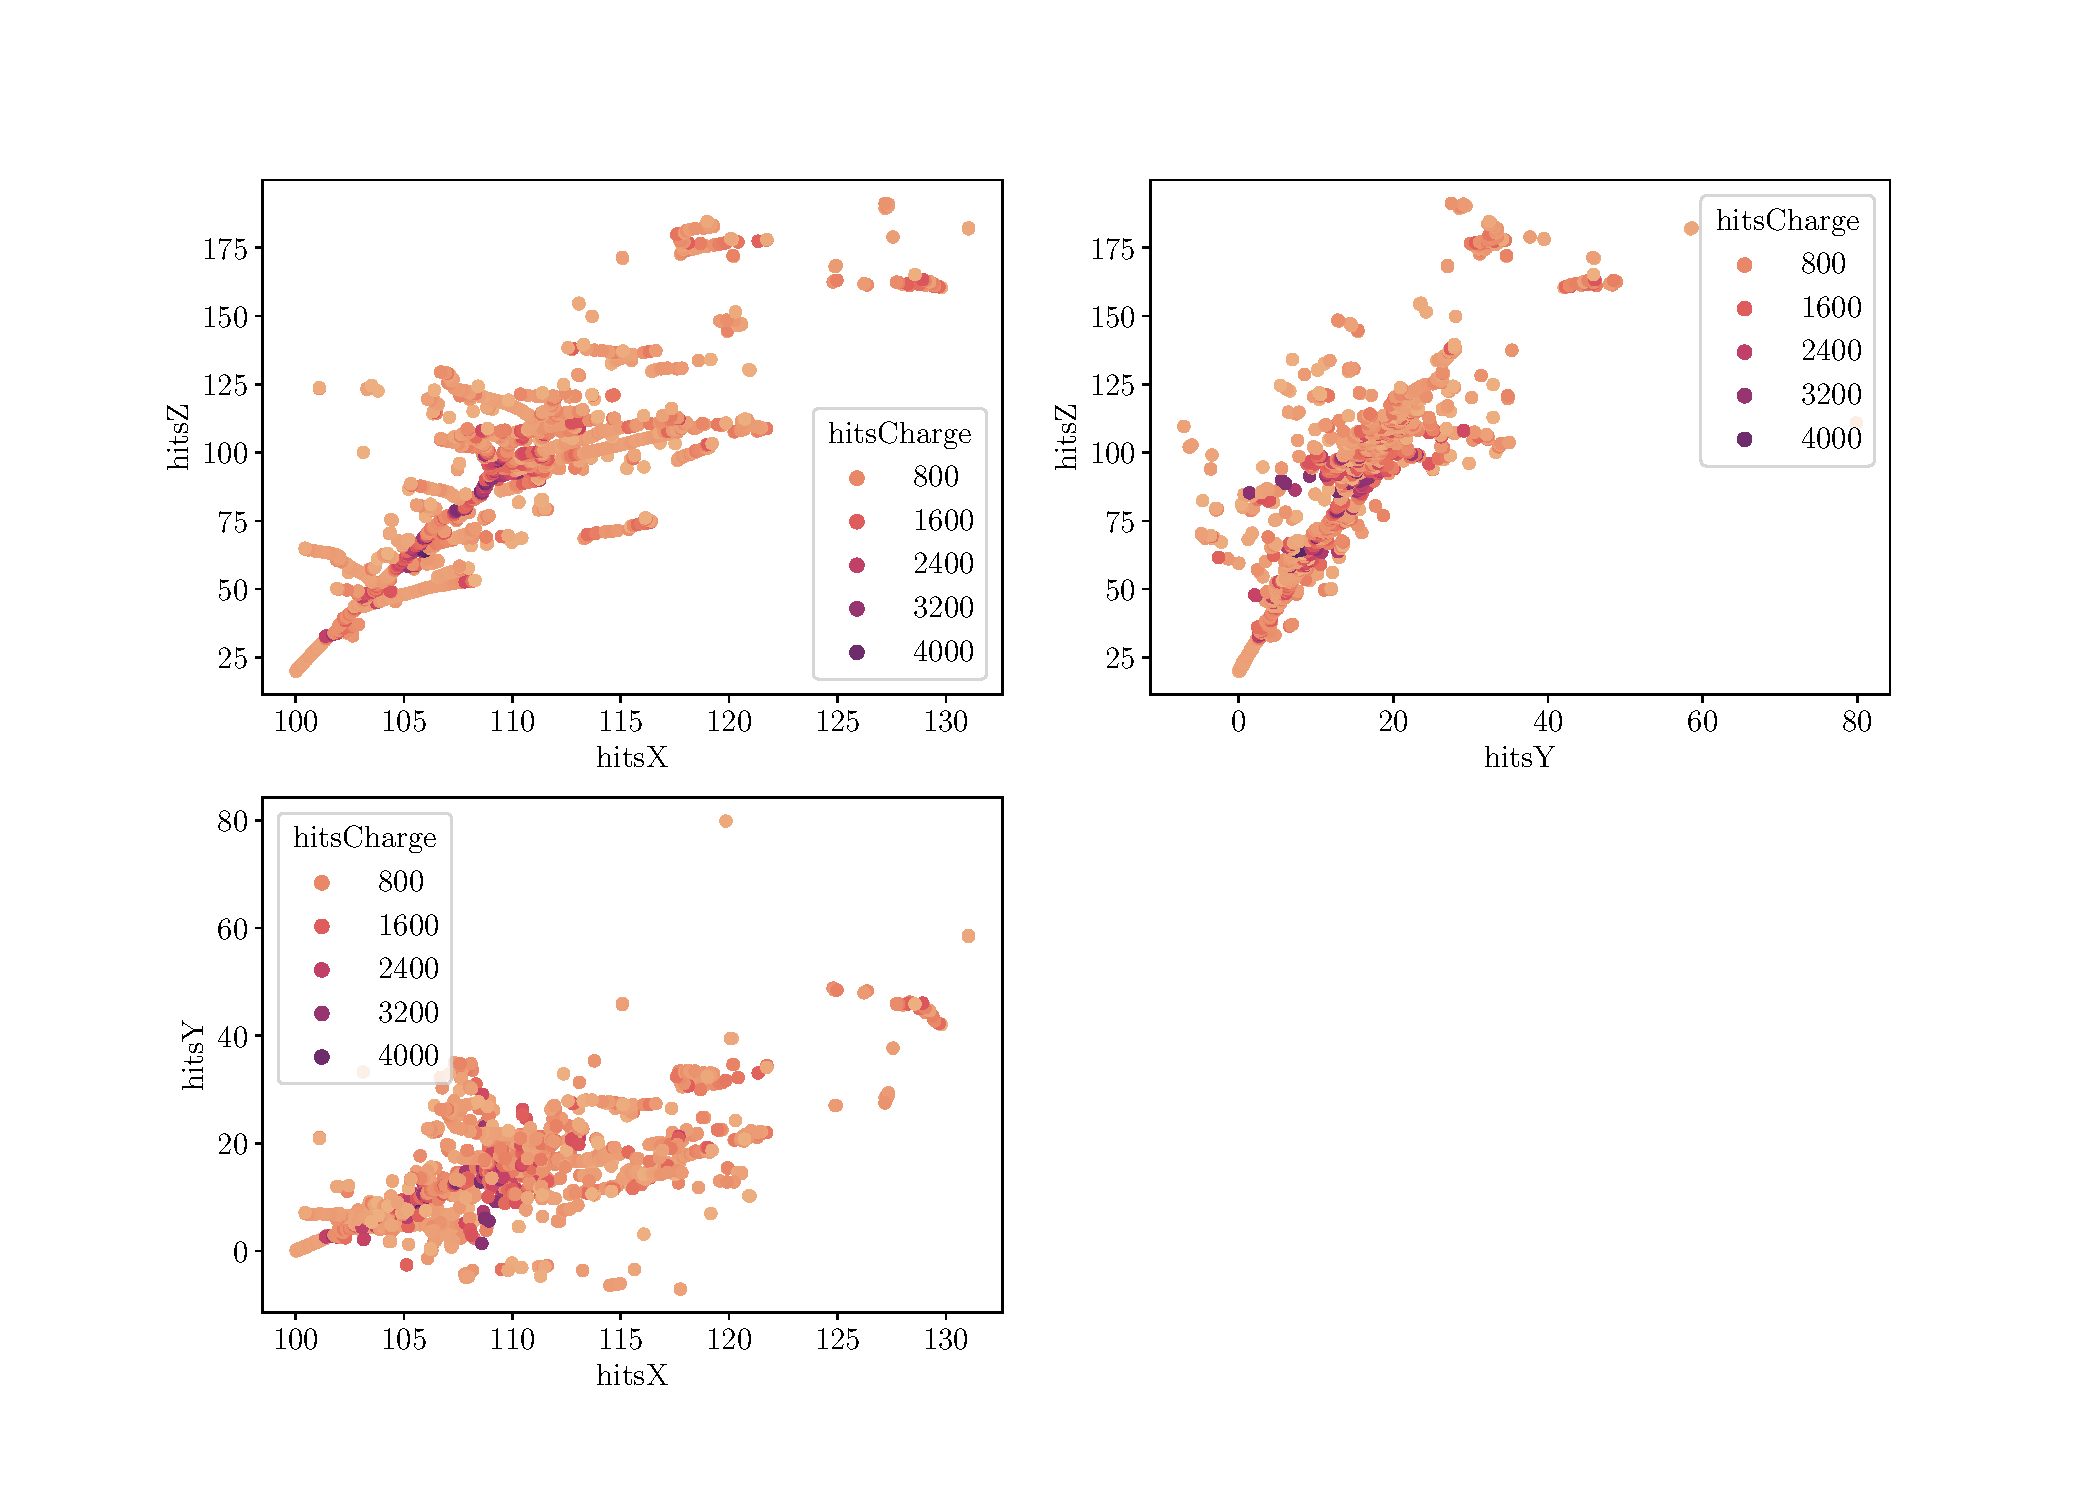
\includegraphics[scale=0.39]{vistas_3.pdf}
  \caption{Representación de las tres vistas de una cascada electromagnética originada por un fotón con los datos en bruto. El color de los puntos viene dado en función de la carga del \textit{hit}.}
  \label{fig:vistas}
\end{figure}


Nuestro objetivo principal en este trabajo es logar distinguir las cascadas originadas por los fotones de las producidas por los electrones y tenemos que ver como abordar este problema desde el punto de vista de la ciencia de datos. Como ya hemos mencionado y visto en distintas gráficas, este detector nos permite reconstruir los eventos como imágenes tridimensionales por lo que podemos abordar este problema como un problema de clasificación de imágenes. Esta no es la única forma de abordar el problema pero es en la que nos vamos a centrar en este trabajo.

Las redes convolucionales son el estado del arte en clasificación de imágenes por lo que todos los enfoques que vamos a desarrollar van a hacer uso de estas arquitecturas. Sin embargo, se pueden abordar mediante otros procedimientos como puede ser hacer la clasificación mediante la definición de nuevas variables a partir de las imágenes o el uso de métodos clásicos de extracción de características. Estos enfoques son más clásicos en el sentido que no se hace uso del Deep Learning y lo que hacemos es definir nosotros las características con la luego aplicar un clasificador.

\subsection{Procesamiento de los datos}
\label{sec:des_trat}
Antes de entrar en los modelo que vamos a usar para hacer la clasificación tenemos que ver cómo  se tratan los datos iniciales para que así podamos hacer uso de un modelo. Lo primero que tenemos que hacer es pasar los datos que tenemos al formato con el que se tratan las imágenes. Una imagen no es más que una matriz donde cada elemento es un píxel. En nuestro caso, al trabajar con imágenes tridimensionales, tendremos que trabajar con matrices con cuatro dimensiones, tres de posición y una para el canal de color. El color de la imagen lo asociaremos con la cantidad de carga depositada por el hit, por lo que, en principio, trabajamos con imágenes en blanco y negro.

Una vez que hemos construido las imágenes vamos a plantear distintas formas de tratarlas que consideramos que pueden ayudar a la hora de discriminar los eventos. Estamos son los que enumeramos a continuación.

\begin{itemize}
  \item Trabajar directamente con las imágenes tridimensionales. Las CNN no están limitadas a trabajar con imágenes bidimensionales, estas pueden trabajar con imágenes de cualquier dimensión. En la Sección \ref{sec:dl} cuando las presentamos, vimos que la operación de convolución se puede generalizar a cualquier dimensión.
  \item Trabajar con imágenes bidimensionales donde nos quedamos únicamente con una proyección. El problema con este enfoque es que se pierde mucha información.
  \item Para solucionar esto lo que podemos hacer es agregar la información obtenida de las tres proyecciones o usando un ensemble o agregando las características obtenidas en los tres modelos.
  \item Codificar la información perdida a la hora de hacer la proyección en forma de color de manera que mantenemos toda la información usando imágenes bidimensionales pero con tres canales de color.
\end{itemize}

Independientemente del modelo o enfoque empleado es necesario pasar los datos tabulares a imágenes pero surgen una serie de problemas al realizar esta conversión. El problema surge con la resolución de la imagen, la posición viene dada en centímetros y tenemos resolución en varias décimas de milímetro. Teniendo en cuenta que las dimensiones son 400x400x500 cm$^3$ tenemos imágenes con muchos píxeles. Notar por tanto que la precisión del detector esta relacionada con la resolución de la imagen, entendiendo resolución de la imagen como el número de píxeles que usamos para representar el volumen completo del detector.

El problema surge si queremos mantener toda esta información, es decir, la resolución, ya que necesitaríamos muchos píxeles y a más píxeles mayor número de parámetros vamos a tener en el modelo. Otra cuestión a considerar es que tenemos un número considerable de filas por lo que tenemos que tener esto en mente a la hora de hacer el cambio, ya que podemos tener problemas de memoria, de hecho, otro punto que se debería considerar en este problema es hacer uso de técnicas de Big Data para abordar el problema, no obstante, nosotros no vamos a entrar en ello al alejarse del objetivo de este trabajo.

Otro punto importante es que es necesario parametrizar cualquier cosa que influya en el procesamiento de las imágenes, no solo para hacer un seguimiento de los mismos, si no también para poder probar con distintas configuraciones. Sobre todo es importante tener como parámetro la resolución final así como el tamaño de la imagen ya que son parámetros que pueden influir mucho en los resultados y eficiencia del modelo.

Veamos cómo vamos a tratar la imágenes. Mencionar que vamos a realizar todo el procedimiento desde cero. Se podría haber hecho uso de la librería matplotlib simplificando mucho el problema, pero esto solo serviría en caso de trabajar con la proyecciones ya que genera las imágenes directamente de los datos tabulares. Debido a que vamos a probar distintos enfoques, vamos a realizar la implementación desde el principio ya que los distintos procesamientos parten de la misma idea y son cambios muy pequeños de una implementación a otra. Además, de esta forma tenemos control total sobre las imágenes y todas van a compartir los parámetros.

Los datos dados están en el sistema de referencia del detector donde el eje $z$ va de 0 cm a 500 cm y los ejes $x$ e $y$ van de -200 cm a 200 cm. Para regular la resolución y pasar los datos a una imagen lo que vamos a hacer es un es aplicar un cambio de sistema de referencia así como de unidades. Con estos cambios lo que pretendemos es regular la resolución así como facilitar la creación de las imágenes.

Para entender la idea que hay detrás de esto pongamos el siguiente ejemplo, supongamos que se tiene una regla que solo tiene marcados los centímetros. Si se empleara para medir el lado de un cuadrado que mide 1.2 \si[]{cm}, al colocar la regla veríamos que el cuadrado acaba entre la marca con el 1 y con el 2, por lo que podemos decir que mide 1 \si[]{cm} con un cierto error al ver que el cuadrado acaba más cerca del 1 que del 2 pero se pasa un poco. Con las transformaciones que planteamos lo que queremos hacer es crear nuestra regla donde el punto más pequeño lo colocamos en el cero y lo que hacemos es aumentar el número de marcas entre el valor más pequeño posible y el valor más grande posible si queremos aumentar la resolución y reducir el número de marcas si queremos reducir la resolución.

Para fijar ideas, supongamos que tenemos solo dos dimensiones y queremos acabar con imágenes 100x100. Para esto lo que hacemos primero es realizar un cambio de referencia de manera que el valor más chico en cada eje pase a ser cero. Ahora lo que hacemos es cambiar las unidades para que el valor más grande en los eje pase a valer 100. Si redondeamos el resultado obtenido para cada punto obtenemos la marca más cercana a dicho punto y que además nos sirve como índice para colocar el píxel en la matriz (la imagen).

De manera formal lo que se tiene es lo siguiente. Sea ${r} = (r_x, r_y, r_z)$ un punto cualquiera de la trayectoria de un evento cualquiera, $t_{min} = (x_{min}, y_{min}, z_{min})$, $t_{min} = (x_{max}, y_{max}, z_{max})$ tuplas que recogen los valores más pequeños y más grande en cada eje respectivamente, que se obtienen de todos los eventos de entrenamiento, y $c = (c_x, c_y, c_z)$ una tupla con la resolución final de la imagen que contiene al detector completo y que verifican:
\begin{equation}
  \label{eq:resolucion}
  c_x = c_y = \frac{5}{4}c_z,
\end{equation}
para que los tres ejes tengan las mismas unidades.

Lo primero que hacemos es aplicar el cambio de referencia (sumar a cada eje una constante a todos los puntos de todos los eventos) con la idea que el punto más pequeño este en origen:
\begin{equation}
  {r}^\prime = {r} - t_{min}.
\end{equation}
Ahora aplicamos el cambio de unidades (multiplicar a cada eje por una constante):
\begin{equation}
  {r}^{\prime\prime} = \frac{{r}^\prime}{t_{max} - t_{min}} \cdot c.
\end{equation}
Finalmente redondeamos $r^{\prime\prime}$ a un entero. Aplicamos esto a todos los eventos y todos los puntos, con lo que finalmente para cada evento tenemos las posiciones dadas con números enteros cuyo mínimo es el cero y el máximo es $c$ obteniendo así los índices de la matriz que representa la imagen.

Esta imagen que hemos obtenido es del detector completo, pero los eventos no ocupan todo el detector por lo que debemos dar una parte de este volumen para evitar tener regiones muy vacías, una venta. Además, estas ventanas tienen que ser iguales para todos los eventos. Para esto tenemos que ver dónde colocamos esta ventana. Una opción sería colocarla en el centro de masas de la cascada, otra opción posible sería situarla al comienzo de la cascada ya que sabemos que hay es donde más diferencias hay entre los dos tipos de cascadas. Otro parámetro que vamos a tener en nuestro modelo final es el tamaño de esta ventana, que no es más que el tamaño final de la imagen.

Como comentario final, es posible que a la hora de hacer el paso de datos tabulares a imágenes, al estar cambiando la resolución, tengamos para el mismo punto del espacio dos valores distintos de carga por lo que tendremos que elegir un valor. Hay distintas opciones como puede ser tomar el máximo o la media, estas opciones también las introducimos como parámetros.

A modo de resumen la creación de las imágenes consiste en primero obtener los máximos y mínimos de las coordenadas espaciales y de la carga. Con esto hacemos las transformaciones descritas obteniendo los índices para colocar los píxeles en la imagen. Tras la transformación lo que se hace es realizar la proyección correspondiente, que puede ser o quitarnos unos de los ejes, quedarnos con la imagen tridimensional o hacer la codificación de la 3º dimensión en forma de color. Una vez se tienen los indices colocamos la ventana que la situamos de manera que el origen del evento este situado en una esquina inferior de la imagen (en uno de los ejes se tiene que tener cuidado por que dependiendo de en que zona del detector ocurra tendremos que cambiar la esquina).

\subsection{Modelos propuestos}

Una vez se han procesado los datos y tenemos la imágenes tenemos que aplicar un modelo para realizar la clasificación. En esta sección simplemente vamos a enumerar los distintos modelos propuestos para realizar la clasificación:

\begin{itemize}
  \item Una CNN simple, con pocas capas que nos sirva de punto de partida.
  % \item \red{Una CNN compleja hecha por nosotros????}
  \item Una CNN más compleja, similar a la simple pero más densa, más filtros y neuronas, y más profundas, más capas.
  \item Hacer uso de arquitectura del estado del arte como pueden ser ResNet, EfficientNet o Visual Transformers. Probaremos a entrenar con los pesos aprendidos con el conjunto de datos de ImageNet reentrenando las últimas capas.
\end{itemize}

Con todo esto proponemos distintos métodos tanto para el procesamiento de los datos así como el modelo empleado. En las siguientes secciones mostraremos tanto una descripción detallada de las arquitecturas de los modelos empleados así como los resultados obtenidos a la hora de hacer la clasificación.

\subsection{Flujo de trabajo}

Sin entrar en los detalles de la implementación, veamos el flujo de trabajo que vamos a seguir. En la Fig. \ref{fig:flujo} se muestra de manera esquemática este flujo de manera simplificada.

\begin{figure}[h!]
  \centering
  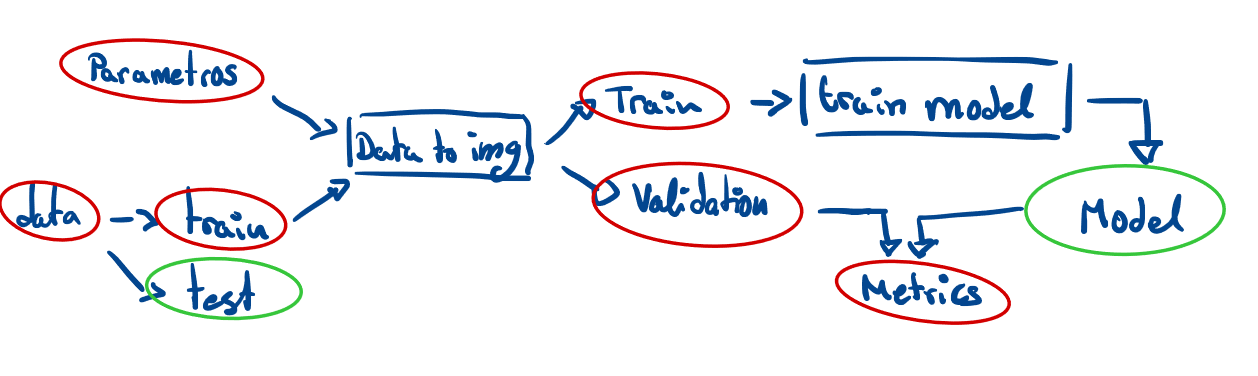
\includegraphics[scale=0.49]{flujo_tem.PNG}
  \caption{Esquema del flujo de trabajo implementado para resolver el problema de clasificación de cascadas electromagnéticas. Los cuadrados son bloques de código mientras que las elipses representan datos, parámetros y modelos. En rojo se índica que es forma parte del proceso de entrenamiento y validación mientras que en verde se recoge lo que se despliega tras el entrenamiento.}
  \label{fig:flujo}
\end{figure}

Se parte de los datos proporcionados y de los parámetros del modelo así como para tratar las imágenes. Lo primero que hacemos es separar el conjunto de entrenamiento en entrenamiento y prueba de manera que nos aseguramos que nuestro modelo no hace uso del conjunto de prueba en ningún momento. En este punto lo que hacemos es pasar el conjunto de datos a imágenes que volvemos a separar en entrenamiento y validación. Con las imágenes de entrenamiento entrenamos un modelo haciendo uso de los parámetros dados y evaluamos el modelo usando el conjunto de validación. El modelo final es guardado junto con los parámetros para su uso futuro.

Este flujo mencionado esta muy simplificado, veamos algunas cosas que son importantes mencionar. A la hora de entrenar el modelo, como estamos usando redes neuronales, en el entrenamiento damos varias vueltas por el conjunto de entrenamiento y validamos en cada vuelta hasta obtener el mejor modelo usando los resultados de validación para elegir el modelo final. Otra cosa que no se muestra en el flujo es que para el procesamiento de los datos necesitamos obtener el mínimo y máximo de varias magnitudes por lo que al aprenderlas con el conjunto de entrenamiento estas tienen que guardarse con el modelo para poder procesar imágenes futuras.

Otro aspecto importante es que tenemos un conjunto de parámetros que vamos a tener explorar para obtener los mejores resultados. Para esto hacemos uso de la librería Optuna que nos permite hacer esta búsqueda de manera más eficiente que haciendo una búsqueda de rejilla, al tratar de optimizar una función objetivo. Para esto partimos del flujo descrito y lo que hacemos es una vez validado el modelo, en función del resultado obtenido por la función objetivo modificamos los parámetros de manera iterativa.

Por otro lado, como ya se menciono al estar trabajando en un problema donde no se esta trabajando con un equipo que se mezclen el desarrollo y operaciones hay puntos donde no tiene sentido hacer uso de algunas técnicas de MLOps, sobre todo, una vez obtenido el modelo. En nuestro caso las prácticas que hemos llevado a cabo son:
\begin{itemize}
  \item Encapsulación de las distintas partes de flujo de manera que cualquier modificación realizada no afecte al flujo teniendo así un sistema de tuberías.
  \item Todos los modelos entrenados, junto con sus resultados y los parámetros han sido guardados haciendo uso de MLFlow. Una herramienta que facilita mucho tanto el despliegue como el seguimiento de los resultados.
  \item Para simular el despliegue lo que se ha hecho es simplemente construir un flujo que parta de datos nuevos (en nuestro caso el conjunto de prueba) y el modelo aprendido y clasifique los datos. 
  \item Se ha realizado la implementación para que para hacer el entrenamiento solo sea necesario indicar los parámetros y para la evaluación de nuevos datos solo se requiera indicar el modelo que se quiere usar.
\end{itemize} 
\newpage
\section{Análisis de los datos}

En esta sección vamos a analizar los datos con la idea de poder entenderlos mejor y poder tomar decisiones sobre como procesar los datos y crear las imágenes. En concreto nos centraremos en estudiar el rango y distribución de distintas variables.

Como ya se ha mencionado, una de las variables que tenemos para cada evento es la energía de la partícula que origina la cascada. Recordemos que esta variable se tiene gracias a que trabajamos con simulaciones y solo se usará para hacer el estudio de los resultados obtenidos. En la Fig. \ref{fig:hist_energia} se muestra un histograma de la distribución de energías de los distintos eventos donde vemos que se tiene una distribución uniforme, es decir, no hay rangos de energía donde se tengan más eventos. En nuestro caso, se tiene esta distribución al trabajar con simulaciones y nos permite entrenar la misma cantidad de evento en los distintos rangos de energía. En la realidad no se espera que los datos sigan esta distribución por lo que será necesario estudiar las métricas en función de la energía para saber si hay rangos de energía donde nuestro modelo es mejor o peor.

\begin{figure}[h!]
  \centering
  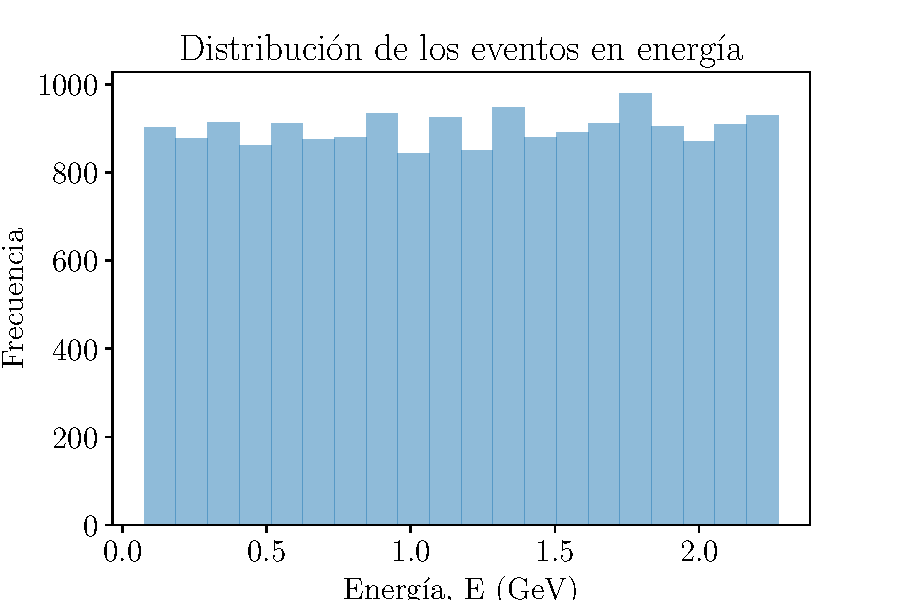
\includegraphics[scale=0.85]{hist_en.pdf}
  \caption{Histograma de la energía de los distintos eventos.}
  \label{fig:hist_energia}
\end{figure}

Otra variable que resulta importante comprender es la posición, en concreto nos interesa saber la cantidad de volumen que ocupan los eventos, ya que nos permite entender el efecto que tienen en la imagen la resolución y el tamaño de la ventana. Para obtener el volumen lo hacemos es agrupar por eventos y calcular el rango en los distintos ejes para cada evento, es decir, para cada evento restamos el máximo y el mínimo en cada eje, obteniendo así el rango para los tres ejes para cada evento. En la Fig. \ref{fig:hist_rango} se muestran los histogramas para estas nuevas variables. Por otro lado, en la Tabla \ref{tab:cuartiles_rango} mostramos los cuartiles para estas mismas variables.

\begin{figure}[h!]
  \centering
  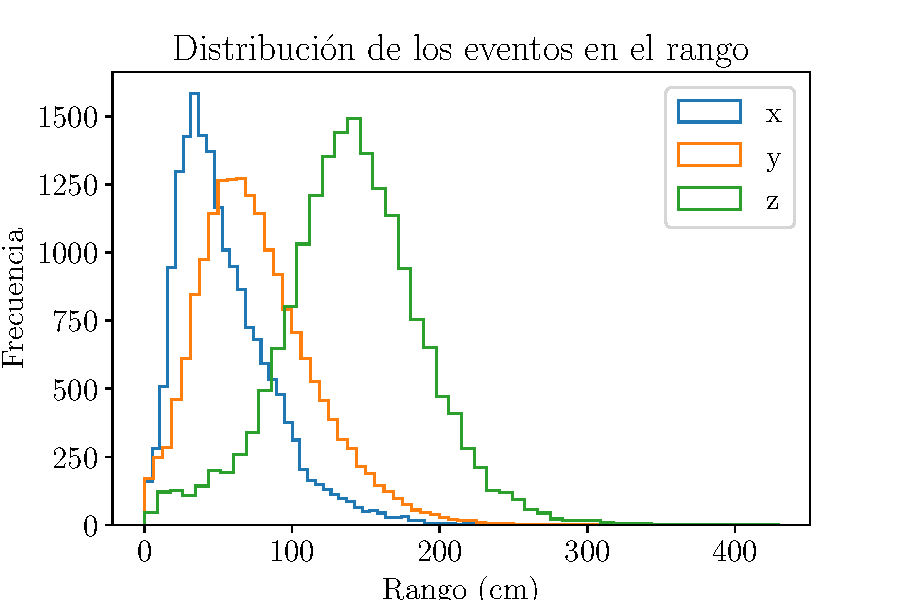
\includegraphics[scale=0.85]{hist_rango.pdf}
  \caption{Histograma de los rangos. Los rangos hacen referencia a la distancia entre el \textit{hit} que ocurre en el valor más pequeño y el ocurre en el valor más grande. Se obtienen para los tres ejes espaciales y para cada evento.}
  \label{fig:hist_rango}
\end{figure}

\begin{table}[h!]
  \centering
  \begin{tabular}{|c|c|c|c|}
  \hline
           &  hitsX (cm) &  hitsY (cm) &  hitsZ (cm) \\ \hline
  min      &        0.04 &        0.00 &        0.40 \\ \hline
  25\%     &       31.26 &       48.79 &      111.90 \\ \hline
  50\%     &       47.47 &       71.12 &      140.50 \\ \hline
  75\%     &       72.23 &       98.97 &      170.15 \\ \hline
  max      &      263.51 &      312.29 &      429.40 \\ \hline
\end{tabular}
\caption{Cuartiles de los rangos que alcanzan las cascadas en los distintos eventos y ejes.}
\label{tab:cuartiles_rango}
\end{table}

Antes de entrar a discutir estas gráficas, recordemos que el parámetro $c$ nos permite regular la resolución con la que se describe el volumen del detector. Supongamos que queremos tener una resolución de 0.1 cm, es decir, construir una imagen donde la distancia entre dos píxeles consecutivos equivale a 0.1cm. En este caso teniendo en cuenta las dimensiones del detector: $x \in [-200, 200]$ cm, $y \in [-200, 200]$ cm y $z \in [0, 500]$ cm el valor de $c$ tendría que ser $(4000, 4000, 5000)$ px. Básicamente lo que tenemos que hacer es establecer una resolución y dividir el rango de los ejes por esta resolución. Este valor de $c$ significa que representamos el volumen completo del detector con una malla de $4000\times 4000\times 5000$ px. Un evento dentro de este volumen solo ocupa una parte y lo que hacemos es coger una ventana del volumen completo. Por ejemplo, si queremos una proyección de $128\times 128$ px lo que hacemos es realizar la proyección y quedarnos con una región con estas dimensiones del volumen completo.

En la Tabla \ref{tab:cuartiles_rango} se recogen los cuartiles de los rangos que tienen los distintos eventos. Entonces, si seguimos con el ejemplo anterior, supongamos que queremos asegurarnos que no se pierde nada de información al tomar la ventana, para esto tenemos que ver cual es el rango máximo que puede darse en un evento. En el caso que la resolución sea de 0.1 cm tendríamos que usar imágenes de $2636\times 3123\times 4294$ px que son imágenes muy grandes. Sin embargo, si nos conformamos con mantener la información completa del 75\% de los eventos, el tamaño de la ventana sería de $723\times 990\times 1701$ px que siguen siendo imágenes muy grandes pero son considerablemente más pequeñas. A la hora de entrenar los modelos vamos a tener que jugar con los parámetros de resolución y de tamaño de la ventana para regular la cantidad de información que se mantiene al crear las imágenes. Es importante mencionar que la información que se pierde es, en su gran mayoría, la parte final de cascada\footnote{Debido a la geometría del problema las cascadas tras originarse se desarrollan de menor $z$ a mayor $z$ y en el eje $x$ depende de si ocurre a la derecha o la izquierda del cátodo porque siempre se dirigen hacia el ánodo (recordar Fig. \ref{fig:sensado} y \ref{fig:estructura_detector}). Al crear las imágenes las centramos en el origen colocando el origen en una esquina de manera que se recoja la dirección de avance. Sin embargo, puede darse que en algunas ocasiones las partículas emitidas durante la interacción se dirijan en la dirección contraria dando situaciones en las que se pierde un poco de información no correspondiente al final de la cascada.} mientras que el origen se mantiene siempre. Lo hacemos de esta forma ya que en origen de la cascada es donde se tienen las principales diferencias entre las cascadas electromagnéticas de origen electrónico y de origen fotónico. En la Fig. \ref{fig:varias_resoluciones} se muestra el mismo evento para distintos valores resolución, donde vemos como a para valores muy bajos tenemos toda la cascada pero con muy poca definición de la cascada. Sin embargo, a media que se aumenta vemos como se va definiendo la cascada pero vamos perdiendo información. El tamaño de la imagen mostrada es de de $128\times128$ px.

\begin{figure}[h!]
  \centering
  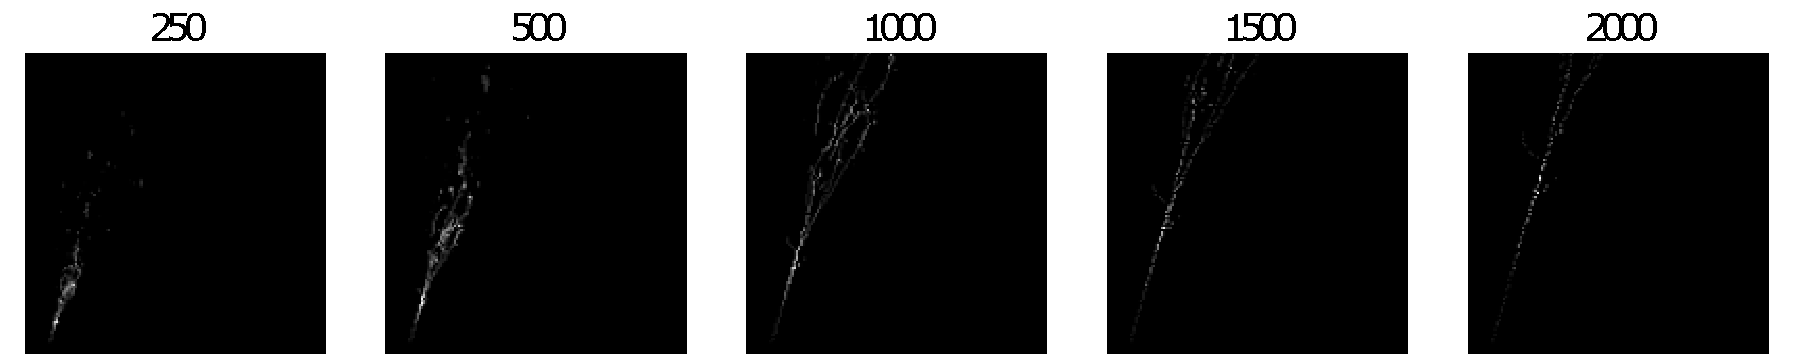
\includegraphics[scale=0.65, center]{varias_resoluciones.pdf}
  \caption{Mismos evento representado para distintas resoluciones (número de píxeles que describen el detector completo). El tamaño de las imágenes es de $128\times128$ px.}
  \label{fig:varias_resoluciones}
\end{figure}


Por último, vamos a estudiar los \textit{hits} y su energía. La cantidad de \textit{hits} que se tienen por evento depende de la energía del suceso en Fig. \ref{fig:scatter_n_e} se muestra la relación que hay entre el número de \textit{hits} de un evento y la energía del mismo donde vemos que se observa una tendencia positiva. El problema se tiene sobre todo cuando se tienen pocos \textit{hits} donde un evento esta dado por 5-10 \textit{hits}, es interesante ver como se comporta nuestros modelos a estos rangos de energía bajos.

\begin{figure}[h!]
  \centering
  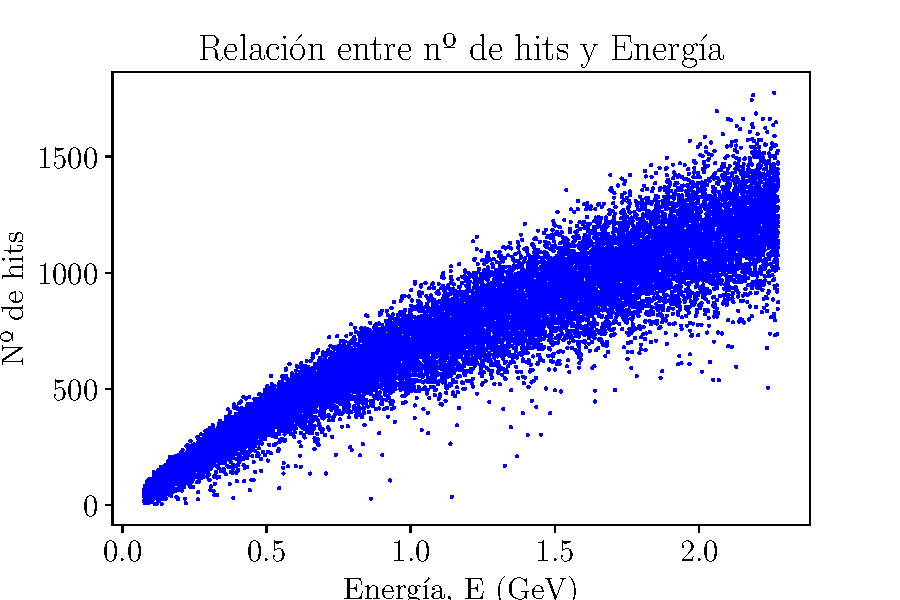
\includegraphics[scale=0.85]{scatter_n_e.pdf}
  \caption{Diagrama de dispersión donde se muestra la relación entre el número de \textit{hits} de un evento y la energía.}
  \label{fig:scatter_n_e}
\end{figure}


Otro aspecto importante es estudiar la carga de cada uno de los \textit{hits} que describen los eventos. En la Fig. \ref{fig:hist_charge} se muestra la distribución de la carga tras dividir por el valor máximo de la carga y también se muestra los mismos datos tras aplicar una transformación logarítmica. En esta gráfica vemos a simple vista que parece que la distribución sin aplicar la transformación logarítmica sigue una distribución exponencial, donde tenemos que la mayoría de \textit{hits} depositan poca carga mientras que muy pocos tienen valores de carga mayores. Sin embargo, vemos que tras aplicar la transformación se pierde esta distribución exponencial y tenemos una distribución que en ciertas ocasiones puede ser deseable al no tener tanta diferencias entre el máximo y el mínimo. Notar que al haber dividido por el máximo hay al menos un \textit{hit} con valor 1 en la carga normalizada.

\begin{figure}[h!]
  \centering
  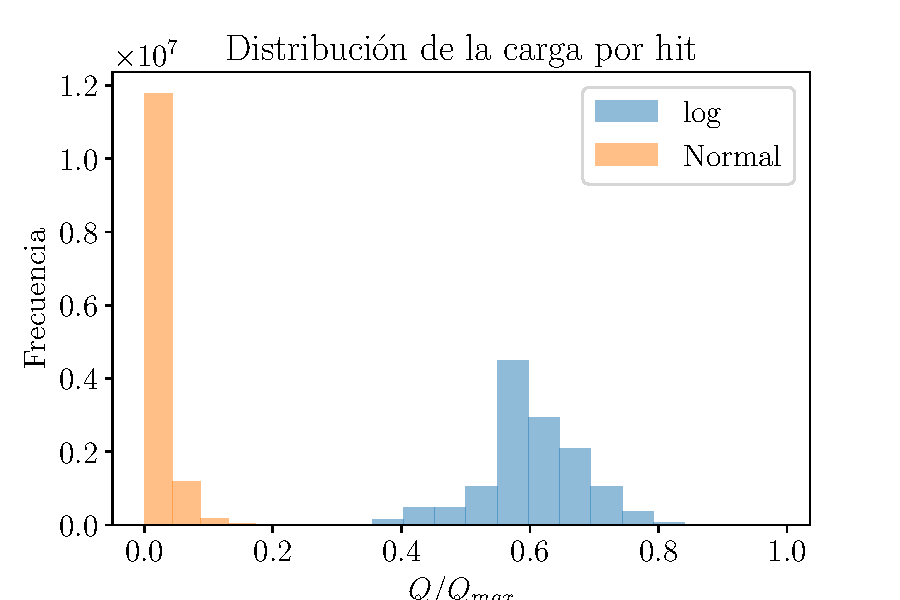
\includegraphics[scale=0.85]{hist_charge.pdf}
  \caption{Histogramas de la carga de los \textit{hits} que se observan en los distintos eventos. Se muestran los datos sin aplicar ninguna transformación y los datos tras aplicar una transformación logarítmica.}
  \label{fig:hist_charge}
\end{figure}


Este comportamiento es importante tenerlo en mente ya que en algunos casos puede que los \textit{hits} más energéticos tengan valores tan grandes que en comparación los menos energéticos no tengan nada de importancia. Una forma de solucionar este problema es haciendo uso de la transformación mostrada. A la hora de entrenar los modelos vamos tener que considerar esta transformación ya que puede que se mejoren los resultados. En algunos caso puede darse que si no se aplica la transformación no se obtengan imágenes que nos permitan describir el evento.

Otra cosa que es interesante observar en esta variable es la distribución de la carga en función del tiempo, ya que es conocido que al comienzo del evento se deben observar valores más altos para la carga. Aunque no se dispone de la variable tiempo, se puede inferir al tener los datos ordenados temporalmente. En la Fig. \ref{fig:hist_charge_t} se muestran un histograma bidimensional donde en el eje $x$ se tiene el tiempo y en el eje $y$ se muestra el logaritmo de la carga. Ambas variables están normalizadas: el tiempo se ha normalizado para cada evento, es decir, un valor de tiempo igual a 0 equivale al comienzo del evento y un valor de 1 equivale al final. Sin embargo, la carga si la hemos normalizado usando el máximo total. Vemos que la distribución en el tiempo es prácticamente uniforme salvo al principio donde vemos que he tienen \textit{hits} con energías superiores.

\begin{figure}[h!]
  \centering
  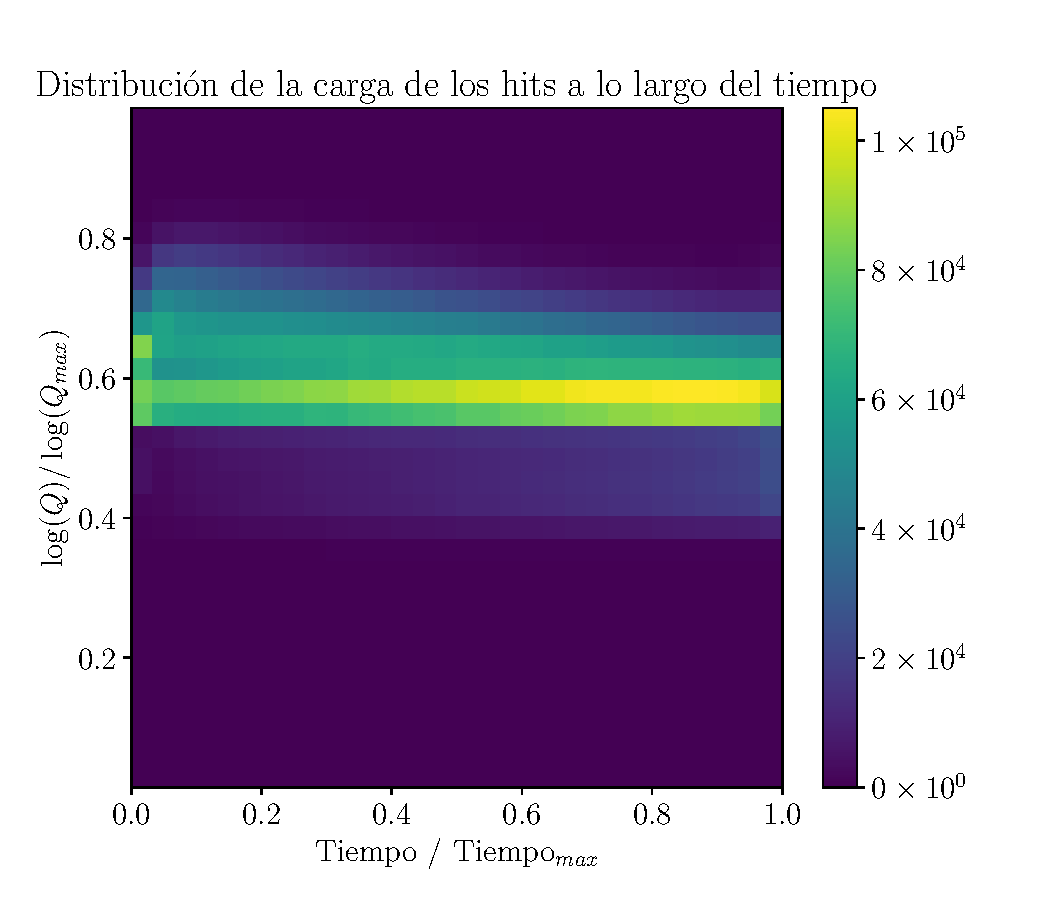
\includegraphics[scale=0.85]{hist_charge_time.pdf}
  \caption{Histogramas bidimensional donde se muestra la distribución de hits en función de la carga y el tiempo. Ambas variables las hemos normalizado para que tomen valores entre cero y uno.}
  \label{fig:hist_charge_t}
\end{figure}


\section{Descripción de la solución}
\label{sec:arch}

En esta sección vamos a recoger y desarrollar todos las propuestas que se plantean en este trabajo. Primero haremos una descripción detallada de las distintas representaciones presentadas. Así mismo, mostraremos las arquitecturas de los distintos modelos que vamos a emplear así como las métricas que emplearemos para realizar el entrenamiento y validar el modelo. Finalmente, haremos un listado de todos los parámetros que tenemos en todo el proceso, desde el tratamiento de los datos hasta el entrenamiento del modelo.

\subsection{Representaciones de los datos}

Como ya hemos visto, hay muchas opciones a la hora de crear las imágenes desde los datos tabulares. En esta sección vamos a describir las representaciones que hemos propuesto. Todas estas representaciones parten de hacer el cambio de unidades y de sistema de referencia que hemos descrito en la Sección \ref{sec:des_trat} secciones anteriores. Lo que vamos a tratar aquí es ver como tratar con la tercera dimensión espacial que no se puede recoger en una imagen. 

\subsubsection*{Representación tridimensional}

Una forma de abordar el problema es quedarnos con toda la información y no descartar ninguna dimensión ya que la operación de convolución no está limitada a trabajar con dos dimensiones espaciales. Esta representación es conceptualmente muy simple pero surgen una serie de problemas como puede ser el tamaño de las imágenes y que no se tienen modelos complejos previamente entrenados como si se tiene para las imágenes bidimensionales.

\subsubsection*{Representación bidimensional, una proyección}

Otra alternativa simple es quedarnos únicamente con una de las proyecciones. De esta forma tenemos una imagen bidimensional. Si recordamos, el eje $x$ es el eje de deriva, el haz de neutrinos está dirigido en la dirección del eje $z$ y eje $y$ es simplemente la altura. En el caso de tener que descartar una de las direcciones la mejor opción es quitar el eje $y$.

La forma de hacer esto es simplemente quitar la columna del eje que se quiera proyectar y en caso de tener eventos repetidos nos quedamos con la media o con el máximo. Por lo demás es simplemente hacer los cambios de unidades y de sistema de referencia. En la Fig. \ref{fig:varias_proyecciones} se muestra gráficamente la trayectoria proyectada de un evento que ha sido obtenida usando los datos tabulares directamente junto con la imagen obtenida tras realizar el tratamiento de datos descrito. Los parámetros que hemos usado para la creación de las imágenes es de $c_x = 1000$ px, de un tamaño de venta de $128\times 128$ px y no aplicar la transformación logarítmica. En la Fig. \ref{fig:muchas_proyecciones} se muestran varias eventos con esta representación, tanto para cascada electrónicas como fotónicas.

\begin{figure}[h!]
  \centering
  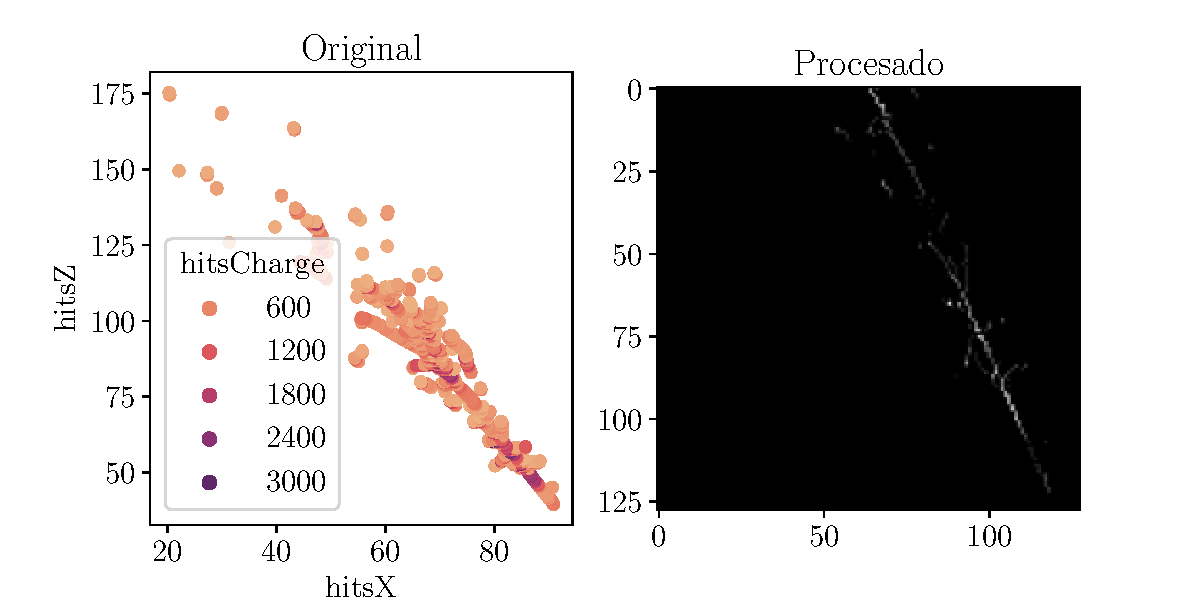
\includegraphics[scale=0.85, center]{ambas_pro.pdf}
  \caption{En la izquierda se muestra un evento proyectado obtenido de los datos tabulares directamente sin hacer uso del procesamiento que presentamos. En la derecha se muestra la imagen procesada con una resolución de 1000 px y tamaño $128\times128$ px.}
  \label{fig:varias_proyecciones}
\end{figure}

\begin{figure}[h!]
  \centering
  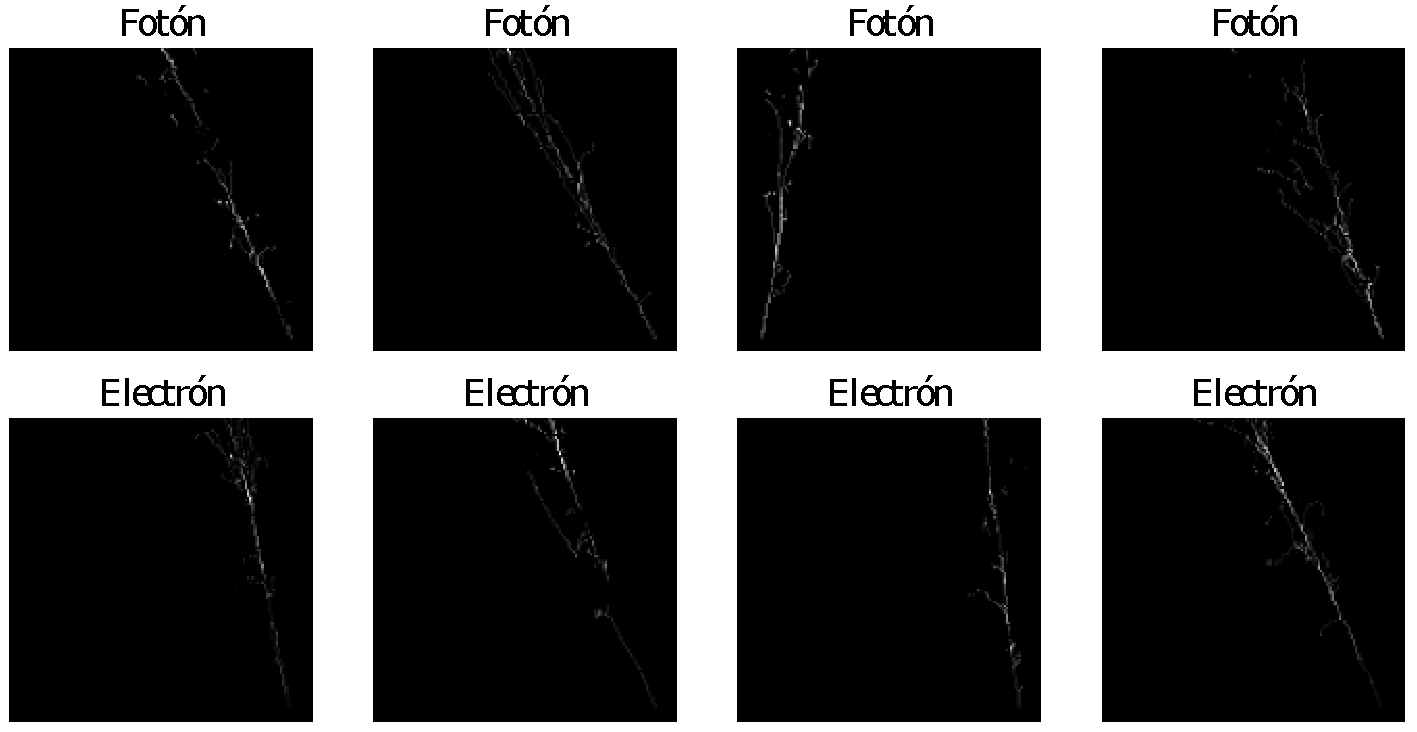
\includegraphics[scale=0.75, center]{varias_proyecciones.pdf}
  \caption{Imágenes obtenidas tras procesar y quedarnos con la proyecciones en el eje $y$ para distintos eventos. Las imágenes han sido procesadas con una resolución de 1000 y tamaño $128\times128$.}
  \label{fig:muchas_proyecciones}
\end{figure}

\subsubsection*{Representación bidimensional, codificación del color}

Al realizar la proyección se pierde completamente la información que se tenía en dicho eje. Una forma de mantener esta información es codificarla de alguna forma en el color de la imagen.

Hasta ahora hemos estado trabajando con imágenes de grises donde la imagen es una matriz con un solo canal. En el caso de trabajar con imágenes que tengan color es necesario trabajar con imágenes que tengan tres canales. Hay distintos espacios para recoger el color de una imagen, el más común es el RGB donde donde los canales recogen la cantidad de rojo, verde y azul de la imagen. Hay otros muchos espacios y en función de lo que se quiera hacer con la imagen será más adecuado usar uno u otro. Nosotros vamos a trabajar en el espacio de color HSL, donde la H hacer referencia al \textit{hue}, el color, la S a la saturación y la L a la luminosidad. En la Fig. \ref{fig:hue} se muestra el color correspondiente para los distintos valores de \textit{hue}. 

\begin{figure}[h!]
  \centering
  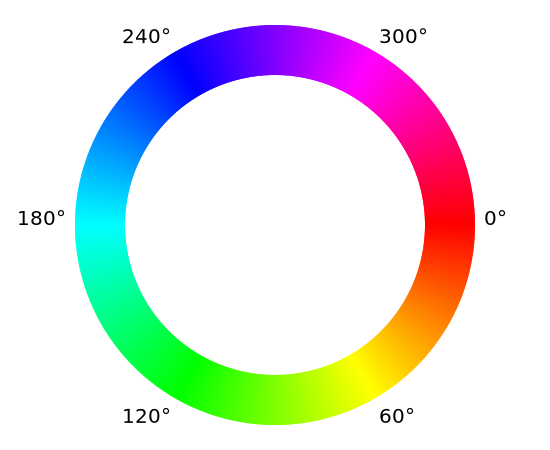
\includegraphics[scale=0.45]{h-colours.png}
  \caption{Rueda con los colores asociados al valor de \textit{hue} fijados la saturación y la luminosidad \cite{hue_page}.}
  \label{fig:hue}
\end{figure}

Si queremos mantener toda la información a la hora de hacer la proyección tenemos que codificar la posición de los \textit{hits} en el eje proyectado así como agregar la carga de los distintos \textit{hits}. Lo que se propone es fijar la saturación, y codificar la posición y la carga en el color y la en luminosidad respectivamente. De esta forma, si se tienen puntos que se superponen en el eje a proyectar lo que hacemos es sumar los valores de la posición en el eje proyectado y de la carga. De esta forma tenemos las dos variables espaciales no proyectadas, la suma de las posiciones en el eje proyectado y la suma de la carga. Estas dos magnitudes obtenidas nos darán el \textit{hue} y la luminosidad.

Veamos esto de manera formal. Sea $X$ el conjunto de datos de partida. Cada instancia hace referencia a un \textit{hit}, y tenemos las columnas $X_e$ que determina el evento del hit, $X_x$, $X_y$ y $X_z$ que indican la posición y $X_c$ que muestra la carga. Para fijar idea supongamos que queremos proyectar el eje $y$. Lo que hacemos es agrupar\footnote{Agrupar consiste en coger todos las instancias que compartan valor en una o varias variables y hacer una operación sobre las variables restantes como puede ser tomar el máximo.} por evento, posición en $x$ y posición en $z$ y sumar tanto la carga como la posición en el eje $y$. Una vez hecho esto lo que hacemos es reescalar las nuevas variables obtenidas de manera que el máximo de la posición sea 180\footnote{Normalmente el rango del \textit{hue} va de 0º a 360º, sin embargo, nosotros vamos a usar Open CV que fija el máximo en 180º.}, al representar el \textit{hue}, y el de la carga sea 1 al representar la luminosidad.

Sea $X^i\left(e = e_n, x=x_m, z=z_p\right)$ los \textit{hits} que pertenecen al evento $e_n$ y están en la posición $(x_m, z_p)$. Definimos $\hat{X}_k$ como:
\begin{equation}
  \hat{X}_k\left(e = e_n, x=x_m, z=z_p\right) = \sum_i X^i_k\left(e = e_n, x=x_m, z=z_p\right) \quad \forall n, m, p.
\end{equation}
Esto es una forma de describir matemáticamente la operación de agrupar por evento y por las posiciones no proyectadas. De esta forma, transformamos los datos a $\hat{X}$ donde las variables por la que hemos agrupado se mantienen iguales y las variables $X_c$ y $X_y$ se han modificado al sumarse aquellas instancias con los mismos valores en las variables agrupadas. Una vez hecho el agrupamiento lo que hacemos es cambiar los rangos para que coincidan con el \textit{hue} y con la luminosidad.

Sin embargo, surgen un par de problemas. Por un lado, si hacemos justo lo que se acaba de mostrar, si tenemos dos eventos idénticos pero solo desplazados en el eje de proyección vamos a tener colores distintos y esto es algo que no queremos que ocurra. Para solucionarlo, lo que hacemos es para cada evento se cambia el sistema de referencia, modificando únicamente el eje proyectado, haciendo cero el mínimo valor del eje proyectado en ese evento. 

El otro problema esta relacionado con la distribución exponencial que se observaba en la carga y que se agrava al realizar la suma. Esto hace que el valor de la luminosidad para la mayoría de eventos sea tan pequeño que al realizar la imagen se tenga que los \textit{hits} no se observan. Para solucionar esto lo que hacemos es tomar logaritmo tras realizar la suma.

Con todo esto lo que vamos a tener en la imagen es valores pequeños de \textit{hue} para el valor más pequeño en el eje proyectado, a medida que la trayectoria se desplace hacia valores más alto en dicho eje, se aumentará el valor del hue. En caso de tener superposición de \textit{hits} observaremos valores más altos en la luminosidad así como en el \textit{hue} al corresponderse a la suma de varios valores de posición y carga. En la Fig. \ref{fig:proy_color} mostramos un ejemplo de un evento tratado con esta representación.

\begin{figure}[h!]
  \centering
  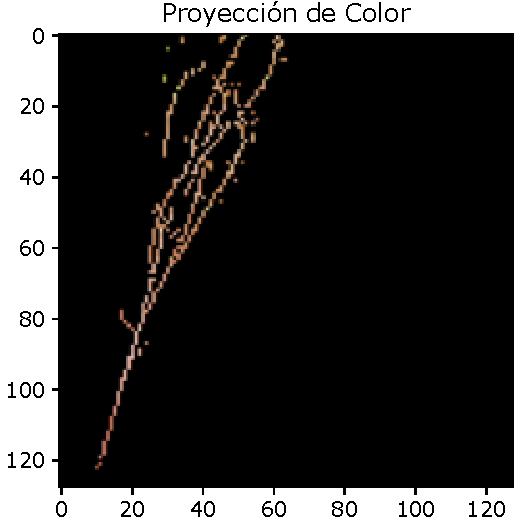
\includegraphics[scale=0.85]{proyeccion_color.pdf}
  \caption{Evento procesado codificando la tercera dimensión en el color de la imagen. Las imágenes han sido procesadas con una resolución de 1000 y tamaño $128\times128$.}
  \label{fig:proy_color}
\end{figure}

\subsubsection*{Representación para Tranformers}

En este trabajo nos vamos a centrar sobre todo en el tratamiento de imágenes y el estudio lo vamos a realizar sobre las imágenes. Sin embargo, también vamos a plantear una representación/tratamiento de los datos distinto que dejamos como trabajo futuro. Nuestros datos tienen un marcado carácter temporal donde tenemos el origen de la trayectoria y esta va avanzando. Además sabemos que al principio es donde se tiene la mayor parte de la información. Los transformers son una arquitectura que ha mostrado muy buenos resultados con texto que son datos donde el orden de las palabras es fundamental. 

Estas redes se basan en hacer uso de mecanismos de atención y codificar la posición de las palabras. Estas redes se han convertido en el estado del arte del procesamiento de lenguaje natural y también se han aplicado en la clasificación de imágenes segmentando la imagen en bloques. La idea es probar a usar los datos tabulares directamente codificando las instancias por el tiempo.

Lo que si haremos es probar el modelo Visual Tranformers (ViT) que hace uso de los tranformers para trabajar con imágenes. Este modelo lo que hace es particionar la imagen y usar estos bloques como entrada para el tranformer. Sin embargo, los datos admiten ser tratados directamente por transformers sin necesidad de pasar por la construcción de la imagen. Por lo que esta forma, de funcionar sería mucho más eficiente que el tratamiento con imágenes y no se descartaría nada de información. 

\subsection{Arquitecturas}

En esta sección vamos a mostrar las distintas arquitecturas que vamos a emplear para realizar la clasificación de las imágenes. Para esto vamos a usar redes diseñadas desde cero así como arquitecturas del estado del arte ya entrenadas donde modificaremos tanto los pesos como el clasificador. Las arquitecturas que usaremos serán: EfficientNet, ResNet, GoogleNet y además vamos a diseñar una red simple y una más compleja basadas en LeNet.

Independientemente de la arquitectura que se use, es necesario implementar el aprendizaje ($lr$) del modelo. Como ya hemos dicho vamos a emplear Pytorch y vamos a considerar un $lr$ dinámico. Para esto necesitamos definir un optimizador, como puede ser SGD o Adam, y la forma de modificar el $lr$. Con esto elementos se implementa primero el descenso del gradiente para todos \textit{batchs} y repetimos esto varias veces para el conjunto de datos (es lo que se conoce como épocas). Cada vez que se completa una época se validan los resultados usando una parte del conjunto de datos no visto por el modelo durante el entrenamiento. A mediad que se avanza en el entrenamiento se van guardando los pesos aprendidos pero solo se guardan se mejoran los resultados en validación, es decir, que los pesos del modelo guardado tras el entrenamiento son aquellos con los que mejores resultados se han obtenido en validación.

Con la intención de no tener fijar un número de épocas lo que hemos hecho ha sido implementar lo que se conoce como parada temprana y es que si tras un número consecutivo de épocas hay mucho sobre ajuste o el modelo no mejora en validación se para el ciclo de aprendizaje y se guardan los pesos con los que mejores resultados se han obtenido. De esta forma no es necesario fijar el número de épocas ya que el entrenamiento se interrumpirá en el momento que ya no estén mejorando los resultados. En el Anexo \red{ref} se muestra la en mayor detalle la implementación realizada del ciclo descrito.

\subsubsection*{LeNet}

LeNet es una de las primeras propuestas de redes convolucionales \cite{lenet} y consiste únicamente en aplicar varias veces el bloque convolucional que se mostró en la Sección \ref{sec:dl} y que consiste en una primera capa que realiza la operación de convolución y una segunda capa de reducción. Una vez se extraen las características se realiza la clasificación haciendo uso de un MLP.

Con estas redes la idea es construir modelos simples que nos permitan establecer un punto de partida que tratar de mejorar con distintas redes o ajustando los hiperparámetros. Crearemos dos modelos basados en esta arquitectura, uno simple y otro más complejo donde se aumentará tanto la anchura como la profundidad del modelo simple. Para hacer el diseño de estas redes lo que hemos hecho es hacer uso de la representación más simple que hemos planteado, la proyección simple, y probar a modificar el número de filtros por nivel así como la el clasificador.

Las pruebas realizadas serán descritas en la Sección \ref{sec:pruebas_iniciales} pero mencionar que nos ha dado muchos problemas la construcción de la red ya que en muchos casos las redes no superaban el 50\% de acierto y pequeños cambios en la estructura de la red hacía que modelo pasara de no aprender a aprender. En la Fig. \ref{fig:lenet} se muestran las arquitecturas de los modelos finales que vamos a usar. Tenemos un modelo simple que consiste en dos bloques convolucionales con pocos filtros y una MLP con dos capas ocultas y pocas neuronas. El modelo más complejo es similar al simple pero hemos modificado el bloque convolucional de manera que se aplican dos capas convolucionales consecutivas sin aplicar la capa de reducción. Además lo que hacemos es tener más filtros y más profundidad y anchura en el MLP.

\begin{figure}[h!]
  \centering
  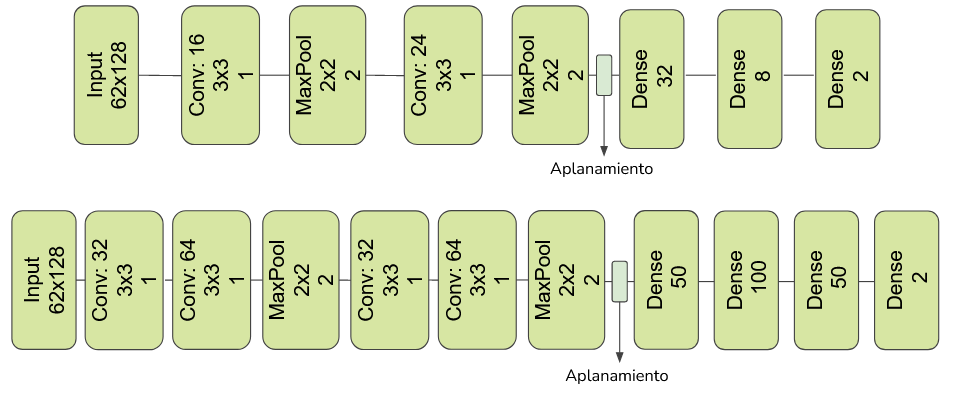
\includegraphics[scale=0.85, center]{lenet.PNG}
  \caption{Arquitectura basada en LeNet usada para la clasificación de las imágenes dadas. En las capas de convolución se muestran el número de filtros, el tamaño y es desplazamiento, en las capas de reducción se muestra el tamaño y desplazamiento y en las capas densas el número de neuronas.}
  \label{fig:lenet}
\end{figure}

\subsubsection*{EfficientNet}

EfficientNet \cite{enet} es una red que ha mostrado dar muy buenos resultados cuyo objetivo es el que sea eficiente y escalable. Uno de los problemas fundamentales que se presentaban tras las primeras CNN es que al aumentar la complejidad de los modelos se tenían problemas para realizar el entrenamiento. Con el paso del tiempo se fueron introducido mecanismos para lidiar con este problema y EfficientNet establece una familia con 8 modelos que parten de un modelo base y van aumentando la complejidad.

Una red neuronal se puede escalar aumentando la profundidad, la anchura o la resolución (tamaño de las imágenes) y EfficientNet lo que hace es introducir un método de escalado que aumenta la complejidad aumentando las tres opciones simultáneamente. Parten de la premisa que las distintas formas de escalar están relacionadas, i.e si tenemos imágenes más grandes vamos a necesitar más filtros y más capas para conseguir realizar la clasificación \cite{enet}.

% La arquitectura del modelo esta basada en MovilNet v2 \cite{} y ademas hace uso de bloques 

Nosotros vamos a usar estas arquitecturas no solo porque han mostrado dar muy buenos resultados en conjuntos de datos complejos si no porque nos permite probar con una red con distintos niveles de complejidad. 

\subsection*{ResNet}
ResNet es una arquitectura que surge antes que EfficientNet e introduce un mecanismo para solucionar problemas a la hora de realizar la optimización cuando se tienen modelos muy profundos \cite{resnet}. Esta basada en VGG \cite{vgg} que se basa en aplicar sucesivamente bloques convolucionales pero teniendo un modelo muy profundo. ResNet introduce lo que denominan celdas residuales que consisten en agregar la entrada del bloque convolucional a la salida \cite{resnet} a esto le denominan aprendizaje residual y muestran una mejora en la optimización del modelo.

La arquitectura consiste en aplicar sucesivamente bloques convolucionales donde solo se aplica la reducción tras la primera capa convolucional y se introduce el aprendizaje residual. Al igual que para EfficientNet, se tiene una familia de modelos donde lo que varía es la profundidad del modelo. Nosotros usaremos únicamente ResNet 50, donde el 50 hace referencia al número de capas. En la Fig. \ref{fig:resnet} podemos ver la arquitectura de este modelo junto con la de VGG y la arquitectura de ResNet sin el aprendizaje residual.

\begin{figure}[h!]
  \centering
  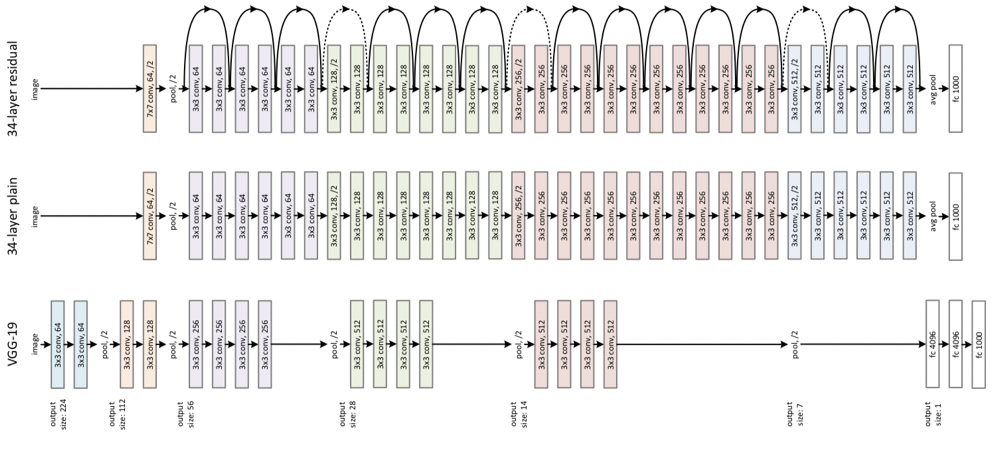
\includegraphics[scale=1.0, center]{resnet50.png}
  \caption{Arquitectura de la red ResNet donde se muestra VGG y como se modifica para introducir el aprendizaje residual.}
  \label{fig:resnet}
\end{figure}

% \subsection*{GoogleNet}

\subsection*{Visual Transformer}

Los transformers \cite{transformers} son modelos que se basan únicamente en mecanismos de atención y actualmente se han convertido en el estado del arte al trabajar con texto. Los Visual transformers hacen uso de esta arquitectura y la aplican a imágenes. La idea fundamental es que dividen la imagen en bloques y tratan cada bloque como una palabra que el tranformers procesa \cite{vit}.

\subsection{Métricas}

A la hora de realizar un problema de ciencia de datos es necesario establecer una métrica que nos diga como de bueno es nuestro modelo para poder mejorar los resultados. Como ya se menciono, en las redes neuronales lo que se hace es definir una función pérdida a la cual se le calcula el gradiente en función de los parámetros de la red y modificar así estos parámetros de la red.

Sin embargo, una vez realizado el ajuste hay distintas métricas que nos permiten que nos permiten evaluar el rendimiento como puede ser el porcentaje de acierto o la curva ROC. Estas métricas nos dan información sobre distintos aspectos pero en física para problemas como el que estamos tratando se suele usar la eficiencia y la pureza.

En un problema de clasificación binaría tenemos dos clases que se suelen denominar como clase positiva y clase negativa. Con el clasificador asignaremos a cada instancia un valor de la clase y pueden darse 4 situaciones:

\begin{itemize}
  \item La instancia sea positiva y el clasificador le asigne la clase positiva. A esto se le denomina positivo real (TP).
  \item La instancia sea negativa y el clasificador le asigne la clase negativa. A esto se le denomina negativo real (TN).
  \item La instancia sea positiva y el clasificador le asigne la clase negativa. A esto se le denomina falso negativo (FN).
  \item La instancia sea negativa y el clasificador le asigne la clase positiva. A esto se le denomina falso positivo (FP).
\end{itemize} 

La eficiencia se define como:
\begin{equation}
  \text{eff} = \frac{\text{TP}}{\text{FN} + \text{TP}},
\end{equation}
es decir, el cociente entre el número de instancias positivas que hemos clasificado bien entre el número de instancias que son realmente positivas.

La pureza se define como:
\begin{equation}
  \text{pureza} = \frac{\text{TP}}{\text{FP} + \text{TP}},
\end{equation}
es decir, el cociente entre las instancias positivas correctamente clasificadas entre las instancias que hemos dicho que son positivas. 

La eficiencia nos dice de todos los eventos positivos se dan en el detector que porcentaje hemos sido capaces de clasificar correctamente. Sin embargo, la pureza nos dice que porcentaje de los eventos que hemos dicho que son positivos son realmente positivos.

En física dependiendo de la tarea que estemos tratando nos va interesar maximizar una u otra. Por ejemplo, en los experimentos donde se pretende descubrir una partícula lo que se quiere normalmente es tener una pureza alta de manera que si se dice que se tiene dicha partícula realmente se tenga. La eficiencia se busca cuando se quiere detectar el número de eventos que ocurren en un detector o cuando no queremos perder datos al realizar la clasificación. Por ejemplo, en un detector Geiger que determina las partículas radiactivas nos interesa que tengamos una alta eficiencia de manera que sepamos cuando es peligroso un sitio.   

\subsection{Hiperparámetros}

Por último, vamos a recoger la mayoría de parámetros que tenemos a la hora realizar el flujo de trabajo completo, que es lo que se conoce como hiperparámetros. Vamos separar clasificar los hiperparámetros en función de que parte del flujo en la que influyen. Vamos a formar tres bloques: El tratamiento de los datos, arquitectura de la red y entrenamiento de la red.

Antes de entrar en estos bloques tenemos algunos parámetros generales como puede ser la semilla aleatoria que nos permite tener una reproducibilidad de los resultados. Es importante tener en cuenta que hay algunas funciones que al usar la GPU para realizar el entrenamiento no son completamente reproducibles, sin embargo, nuestros modelos no hacen usos de estas funciones. Por otro lado, también es posible definir una rejilla de manera que con Optuna se realiza la búsqueda de hiperparámetros dentro de esa rejilla.

Es importante tener en cuenta que el entrenamiento de un red neuronal es algo costoso tanto en recursos como en tiempo por lo que no nos podemos permitir hacer búsquedas en rejillas de gran tamaño. Por esto mismo, es importante seleccionar aquellos hiperparámetros que más pueden influir en los resultados.

\subsubsection*{Tratamiento de los datos}

A la hora de hacer la creación de las imágenes hay un conjunto de parámetro que tenemos que establecer y que en algunos caso afecta mucho en el resultado obtenido. Los parámetros que tenemos son:

\begin{itemize}
  \item \inline{cube_shape_x}: Fija el valor de $c$ en el eje $x$. A partir de este obtenemos los valores en el eje $y$ y $z$.
  \item \inline{win_shape}: Tamaño de la ventana cogida del detector.
  \item \inline{projection}: Tipo de proyección empleada. Como opciones tenemos:  las imágenes tridimensionales, la proyección en cualquiera de los ejes o el tratamiento de color.
  \item \inline{projection_pool} y \inline{cube_pool}: Tratamiento de las situaciones en las tengamos superposición de puntos al realizar el tratamiento. Podemos elegir el máximo o la media.
  \item \inline{log_trans}: Si hacemos o no una transformación logarítmica sobre la carga de los \textit{hits}.
  \item \inline{transform}: Si queremos aplicar una transformación sobre la imagen final. Consiste en hacer uso de la librería \textit{torchvision} que introduce un conjunto de transformaciones como puede ser normalizar lo datos.
\end{itemize}

\subsubsection*{Arquitectura}

Por otro lado se tienen distintos parámetros que nos permitan controlar la red que estamos usando para realizar la clasificación. Estos parámetros dependerán de si el modelos es un modelo de la literatura, donde solo vamos a poder controlar el clasificador y el número de capas a reentrenar , o si es un modelo que se construye de cero, donde lo que hemos hecho es crear un modelo que acepte como parámetros las formas del extractor así como del clasificador. Los parámetros que tenemos para este apartado son:

\begin{itemize}
  \item \inline{model_name}: Nombre del modelo que vamos a usar.
  \item \inline{conv filters}, \inline{conv_sizes}, \inline{convstrides}: Tupla que definen el número de capas convolucionales y como son estas capas: número de filtros, tamaño de los filtros y desplazamiento de los filtros.
  \item \inline{pool_sizes} y \inline{pool_strides}: Define el tamaño y el desplazamiento al realizar el \textit{pool}. Son tuplas y tienen que tener el mismo tamaño que los parámetros que definen la convolución.
  \item \inline{clf_neurons}: Tupla con el número de neuronas por cada capa. Cada elemento de la tupla establece una capa.
  \item \inline{clf_no_linear_fun} y \inline{conv_no_linear_fun}: funciones no lineales aplicadas tras las capas densas y las capas de convolución respectivamente.
  \item \inline{bn}: si aplicamos capas de normalizan por \textit{batch}
  % \item n channel: número de canales de la imagen. En caso de tener
  \item \inline{dropout}: Porcentaje de \textit{dropout}. 
\end{itemize}

\subsubsection*{Entrenamiento de la red}

Por último, tenemos una serie de parámetros que nos permiten regular como se realizar el entrenamiento como puede ser el número de épocas o el tipo de optimizador:

\begin{itemize}
  \item \inline{batch_size}: Tamaño del \textit{batch}.
  \item \inline{n_epochs}: núemro de épocas.
  \item \inline{optim_name}: tipo de optimizador.
  \item \inline{optim_lr}: ritmo de aprendizaje.
  \item \inline{scheduler_name}: En caso de querer tener un ritmo de aprendizaje que cambie con las épocas cual queremos aplicar.
  \item \inline{scheduler_step_size}: cada cuanto se modifica el ritmo de aprendizaje.
  \item \inline{scheduler_gamma}: cuanto se modifica el ritmo de aprendizaje.
\end{itemize}

Podemos ver que tenemos una gran cantidad que podemos modificar y en muchos casos pequeñas modificaciones sobre los parámetros hacen que pasemos de tener modelos que no pasen del 50\% de acierto a modelos que lleguen al 80\% de acierto. Por estos motivo el ajuste de estos hiperparámetros es uno de los aspectos más importantes para tratar de obtener un modelo que nos de buenos resultados. Para esto lo que haremos es trabajar una metodología concreta que nos permita llegar a ciertas conclusiones y luego ajustar solo los parámetros más relevantes.

\subsection{Entorno de trabajo}

Por último, vamos a describir algunas peculiaridades del entorno donde hemos realizado lo experimentos, que es un aspecto importante al trabajar con redes neuronales debido a la gran cantidad de recursos que necesitan. Por un lado, vamos a trabajar con redes neuronales y el entrenamiento de estas redes se beneficia de la gran paralelización de las GPU, sin embargo, el entrenamiento consume muchos recursos lo que hace que en algunos casos un ordenador personal no sea suficiente. La pruebas iniciales se han realizado en un ordenador personal pero para las pruebas finales hemos recurrido a un cluster de ordenadores. 

El otro aspecto fundamental es el control de todas los resultados obtenidos ya al final se van a realizar muchas pruebas y es necesario mantener un seguimiento, no solo por conocer los resultados de pruebas antiguas si no para poder recuperar los modelos que han mostrado buenos resultados y saber los hiperparámetros de este modelo. Como ya hemos mencionado, vamos a hacer uso de MLFlow para hacer este seguimiento así como herramienta que nos permite realizar un despliegue automático de modelos. Además esta herramienta nos ha permitido que al hacer uso del cluster para establecer un servidor donde se guarden todas las métricas y modelos y accesible desde distintas las distintas máquinas\footnote{Para usar el cluster fue necesario hacer una migración de la base de datos que se tenía en local a la nueva base de datos que se creo en el cluster.}. 

\section{Metodología}

En la sección anterior se ha mostrado la gran cantidad de hiperparámetros que tenemos por lo que hacer una búsqueda por todos los parámetros es completamente prohibitiva. Teniendo esto en mente vamos a definir una metodología que nos permita discernir que representación de las que se plantean es mejor así como la resolución de las imágenes. Una vez tengamos indicios que una de las resoluciones es mejor haremos distintas pruebas sobre los modelos que nos permitan mejorar los resultados.

Lo primero que haremos es realizar un conjunto de pruebas no estructurado que nos permiten entender el problema y ver que el tratamiento diseñado es correcto. Así mismo, haremos uso de estas representaciones para diseñar los modelos que funcionen bien y que usaremos para realizar pruebas futuras.

El siguiente punto será determinar cual de las representaciones que presentamos es mejor. Para esto lo que vamos a hacer es probar las distintas representaciones para distintos modelos. En concreto haremos uso de un modelo simple y uno complejo diseñado por nosotros, distintos modelos EfficientNet, ResNet y GoogleNet. La pruebas las haremos de manera que se compartan todos los parámetros y que lo único que vamos a modificar, en caso de ser necesario, son los parámetros del entrenamiento como puede ser el ritmo de aprendizaje. Una vez hecho este análisis se pretende obtener una representación que sea mejor que resto y será la que usaremos para el resto de pruebas. 

El siguiente paso sera establecer una resolución para ello repetiremos el estudio anterior pero lo que cambiaremos ahora es simplemente la resolución. El siguiente paso será ajustar los modelos para intentar superar los resultados obtenidos. Para esto definiremos una rejilla sobre la que buscaremos que parámetros funcionan mejor y lo haremos para distintos modelos.

Una vez hemos obtenidos buenos modelos haciendo uso de la representación establecida trataremos de mejorar los resultados introduciendo modelos más complejos como pueden ser concatenación de redes, o ensembles que nos permitan mejorar los resultados.

\section{Resultados y discusión}

En esta sección vamos a mostrar los resultado de hacer uso los distintos modelos que se han presentado junto con las distintas representaciones. Inicialmente se mostraran las pruebas preliminares realizadas sin una metodología clara pero nos permite entender el problema, su complejidad y establecer un punto de partida. Luego se realizaremos unos estudios que nos permitan determinar tanto la representación como la resolución de las imágenes. Finalmente, ajustaremos los parámetros de los modelos que mejores resultados nos hayan dado y haremos distintas modificaciones sobre los modelos para tratar de mejorar los resultados.

\subsection{Pruebas iniciales}
\label{sec:pruebas_iniciales}
Tras obtener las representaciones y las imágenes vamos a realizar unos primeros estudios para ver que el procesamiento realizado es correcto y tratar de establecer redes capaces de realizar la clasificación. En estas pruebas iniciales no hemos seguido ninguna metodología concreta en gran medida por la infinidad de puntos de partida posibles.

El punto de partida que establecimos fue hacer uso de la representación más simple y una resolución y tamaño que recoja siempre el comienzo de las cascadas al ser la zona donde más diferencias se encuentran. Además hemos tratado de usar imágenes pequeñas nos permitiera construir un modelo con pocos parámetros y establecer un modelo base. Por lo tanto, para estas pruebas iniciales en general hemos usado imágenes donde hemos proyectado el eje $y$ con un $c_x = 1000$ px y de tamaño $62 \times 128$ px ($62$ píxeles para el eje $x$ y $128$ para el $z$)

Lo primero que hicimos fue diseñar el modelo LeNet simple que se mostró en la sección anterior. La idea de hacer un modelo que no sea especialmente complejo con pocos filtros estaba motivada a que la diferencia existente entre las cascadas no son patrones muy complejos si no que se tratan de patrones simples como líneas. Además un modelo simple consume mucho menos recursos y el aprendizaje es rápido lo que nos permite hacer un mayor número de pruebas. Nuestra idea con estos modelos simples es establecer un modelo base que sea capaz de extraer la máxima información del origen de la cascada.

El primer resultado que se obtuvo fue de 67\% de acierto en validación que se obtuvo con la primera prueba, donde la proyección se hizo sobre el eje $z$. Con estas pruebas, el máximo que se llego a obtener fue de un 88.5\% al realizar cambios en la arquitectura, en como se creaban las imágenes y en algunos parámetros de interés así como el eje de proyección donde se escogió el eje $y$ por se el menos relevante. Entrar a comentar todas estas pruebas realizadas no es especialmente interesante al ser más de 100 pruebas y muchos de los cambios consisten en realizar ajuste en el tratamiento de las imágenes, y cambios en el número de filtros, clasificador, variaciones en el ciclo de aprendizaje, etc.

Sin embargo, si hay algunas cosas que se han observado que son especialmente interesantes de mostrar. Una de las primeras cosas que tratamos de hacer tras obtener un modelo que mostraba buenos resultados fue tratar de escalarlo aumentando tanto el número de filtros como el número de capas. No obstante, nos encontramos con que todos los modelos tenían mucha sensibilidad con la semilla de números aleatorios, y con la arquitectura de la red haciendo que en algunos casos se obtuvieran buenos resultados (entorno al $80\%$) mientras que en otros casos no se conseguía superar el 50\%, que es lo mismo que usar una moneda para realizar la clasificación. 

El hecho que los resultados dependan de la semilla es un problema ya que nos incapacita decir que un conjunto de parámetros es malo ya que puede que simplemente estemos en una semilla mala. Para solucionar este problema lo que se probó fue tratar de modificar el tamaño del \textit{batch} ($bs$) y cada cuanto se modifica el ritmo de aprendizaje ($lr$). Otro parámetro que se modificó fue el optimizador ($optim.$) pero Adam mostraba mejores resultados siempre. El motivo por el que pensábamos que tendría que ser un parámetro relacionado con el aprendizaje es porque el tratamiento de las imágenes no depende de la semilla por lo que al cambiar la semilla lo que modificamos es el orden con el que llegan las imágenes al modelo, el conjunto de validación y como se realiza el descenso del gradiente. Con distintas pruebas observamos que al aumentar tanto el $bs$ como la frecuencia de cambio del ($lr$) se solucionaba este problema.

Otra gran cantidad de prueba se hizo con la idea de obtener modelos basados en LeNet más complejos con la idea de ver si eramos capaces de mejorar los resultados al obtener patrones que el modelo simple no es capaz de determinar. Sin embargo, nos encontramos con que muchos de los modelos probados no conseguían clasificar el conjunto de datos. Debido a esto solo hemos conseguido establecer dos modelos de distinta complejidad que consigan clasificar los datos, la arquitectura de estos modelos se mostraba en la Fig. \ref{fig:lenet}. A la hora de realizar los estudios posteriores vamos a usar estos modelos así como los modelos EfficientNet que tienen distintos niveles de complejidad para ver si modelos más complejos mejoran o empeoran los resultados.

\begin{table}[h!]
  \centering
  \begin{tabular}{|c|c|c|c|c|c|}
  \hline
  BN & log & Normalización & dropout & \begin{tabular}[c]{@{}c@{}}Acc.\\ Mejor Val\end{tabular} & \begin{tabular}[c]{@{}c@{}}Acc.\\ Entrenamiento\end{tabular} \\ \hline
  No & No  & No            & 0.0     & 0.885                                                    & 0.892                                                \\ \hline
  No & No  & Si            & 0.0     & 0.649                                                    & 0.638                                                \\ \hline
  No & Si  & No            & 0.2     & 0.865                                                    & 0.840                                                \\ \hline
  No & Si  & Si            & 0.2     & 0.879                                                    & 0.888                                                \\ \hline
  Si & No  & No            & 0.35    & 0.884                                                    & 0.875                                                \\ \hline
  Si & No  & Si            & 0.35    & 0.638                                                    & 0.87                                                 \\ \hline
  Si & Si  & No            & 0.35    & 0.863                                                    & 0.879                                                \\ \hline
  Si & Si  & Si            & 0.35    & 0.866                                                    & 0.865                                                \\ \hline
  \end{tabular}
  \caption{Estudio del efecto de la normalización, capas de normalización por \textit{batch} (BN) y la transformación logarítmica sobre una misma representación. La representación empleada es la proyección en $y$ y el modelo usado es el LeNet simple.}
  \label{tab:transformaciones}
  \end{table}

Otro aspecto que probamos antes de entrar a realizar los distintos estudios fue a probar aplicar la transformación logarítmica así como introducir capas de normalización por \textit{batch} (BN) \cite{batchnorm}. La introducción de estas modificaciones no mostraron mejoras en los resultados y observamos un aumento en el sobre ajuste llegando a obtener cerca de un 100\% de acierto en el conjunto de entrenamiento. Con el uso del \textit{dropout} se consiguió reducir el sobre ajuste llegando a obtener resultados prácticamente idénticos a los obtenidos sin introducir estas modificaciones por lo que no se observa que sean técnicas que mejoren los resultados. En la Tabla \ref{tab:transformaciones} se muestra un pequeño estudio realizado sobre la proyección, una resolución de 1000 px, y una ventana de $62\times128$ px. En este estudio probamos todas combinaciones de introducir o no las capas de BN, la transformación logarítmica y realizar una normalización sobre los píxeles\footnote{Esta normalización se suele aplicar a las imágenes y suele consistir en aplicar un transformación z-score sobre los distintos canales una vez la imagen esta en el rango 0 y 1. Para realizar esta transformación se toman como media: $(0.485, 0.456, 0.406)$ y como desviación estándar: $(0.229, 0.224, 0.225)$. En nuestro caso la imágenes están en este rango, por lo que solo aplicamos la transformación descrita.} para una misma configuración donde solo hemos modificado el \textit{dropout} si se tenía mucho sobre ajuste. Vemos que los mejores resultados se obtienen cuando no se introduce ninguna de modificaciones mencionadas llegando a obtener resultados similares si solo aplicamos la capa BN pero para ello es necesario introducir mucho \textit{dropout} para reducir el sobre ajuste. Otro aspecto importante es que la BN no mejora los resultados si solo aplicamos normalización y es relevante porque para los modelos preentrenados se suele aplicar esta normalización ya que los modelos se han entrenado con imágenes normalizadas de esta forma. Por todo esto, para los próximos experimentos no vamos a hacer uso de estos elementos y solo realizaremos la normalización para los modelos preentrenados.

\subsection{Selección de una representación}

Las pruebas iniciales nos han servido para entender mejor el conjunto de datos y establecer un punto de partida. Además, la sección anterior, nos ha mostrado la cantidad de pruebas que se pueden hacer para mejorar los resultados poniendo en manifiesto la necesidad de establecer una metodología que nos permita descartar opciones.

Lo primero que vamos a hacer es establecer que representación da mejores resultados de manera general. Para ello lo que vamos a hacer es probar distintos modelos, con distintas complejidades y ver cual de ellas es mejor. Para ello hemos usado los mismos parámetros y redes salvo el ritmo de aprendizaje que se ha modificado solo si el modelo no conseguía superar el 50\%. Las pruebas se han realizado a 10 épocas y con una resolución $c_x = 1000$ px.

En la Tabla \ref{tab:estudio_repre} se recogen los resultados para las 3 representaciones que hemos presentado, donde para la presentación tridimensional no se han realizado pruebas con los modelos preentrenados debido a que son redes entrenadas para imágenes planas. Para los modelos preentrenados hemos usando el mismo clasificador que para el modelo LeNet simple. En el Anexo se puede consultar en detalle los parámetros empleados.

\begin{table}[h!]
  \centering
  \scalebox{0.85}{
  \begin{tabular}{cccccccccc}
  \hline
  \multicolumn{1}{|c|}{}                       & \multicolumn{3}{c|}{Proyección}                                                           & \multicolumn{3}{c|}{Color}                                                                & \multicolumn{3}{c|}{3D}                                                                  \\ \hline
  \multicolumn{1}{|c|}{\% de acierto} & \multicolumn{1}{c|}{train} & \multicolumn{1}{c|}{val.}  & \multicolumn{1}{c|}{mejor val.} & \multicolumn{1}{c|}{train} & \multicolumn{1}{c|}{val.}  & \multicolumn{1}{c|}{mejor val.} & \multicolumn{1}{c|}{train} & \multicolumn{1}{c|}{val.} & \multicolumn{1}{c|}{mejor val.} \\ \hline
  \multicolumn{1}{|c|}{Simple}                   & \multicolumn{1}{c|}{0.892} & \multicolumn{1}{c|}{0.885} & \multicolumn{1}{c|}{0.885}      & \multicolumn{1}{c|}{0.763} & \multicolumn{1}{c|}{0.772} & \multicolumn{1}{c|}{0.772}      & \multicolumn{1}{c|}{0.637}     & \multicolumn{1}{c|}{0.627}    & \multicolumn{1}{c|}{0.627}           \\ \hline
  \multicolumn{1}{|c|}{Complejo}                 & \multicolumn{1}{c|}{0.852} & \multicolumn{1}{c|}{0.866} & \multicolumn{1}{c|}{0.866}      & \multicolumn{1}{c|}{0.856} & \multicolumn{1}{c|}{0.836} & \multicolumn{1}{c|}{0.852}      & \multicolumn{1}{c|}{---}       & \multicolumn{1}{c|}{---}      & \multicolumn{1}{c|}{---}             \\ \hline
  \multicolumn{1}{|c|}{EfficientNet B0}          & \multicolumn{1}{c|}{0.762} & \multicolumn{1}{c|}{0.756} & \multicolumn{1}{c|}{0.768}      & \multicolumn{1}{c|}{0.686} & \multicolumn{1}{c|}{0.641} & \multicolumn{1}{c|}{0.646}      & \multicolumn{1}{c|}{---}       & \multicolumn{1}{c|}{---}      & \multicolumn{1}{c|}{---}             \\ \hline
  \multicolumn{1}{|c|}{EfficientNet B2}          & \multicolumn{1}{c|}{0.688} & \multicolumn{1}{c|}{0.665} & \multicolumn{1}{c|}{0.665}      & \multicolumn{1}{c|}{0.675} & \multicolumn{1}{c|}{0.601} & \multicolumn{1}{c|}{0.610}      & \multicolumn{1}{c|}{---}       & \multicolumn{1}{c|}{---}      & \multicolumn{1}{c|}{---}             \\ \hline
  \multicolumn{1}{|c|}{EfficientNet B5}          & \multicolumn{1}{c|}{0.671} & \multicolumn{1}{c|}{0.613} & \multicolumn{1}{c|}{0.623}      & \multicolumn{1}{c|}{0.659} & \multicolumn{1}{c|}{0.587} & \multicolumn{1}{c|}{0.597}      & \multicolumn{1}{c|}{---}       & \multicolumn{1}{c|}{---}      & \multicolumn{1}{c|}{---}             \\ \hline
  \multicolumn{1}{|c|}{EfficientNet B7}          & \multicolumn{1}{c|}{0.663} & \multicolumn{1}{c|}{0.638} & \multicolumn{1}{c|}{0.643}      & \multicolumn{1}{c|}{0.681} & \multicolumn{1}{c|}{0.601} & \multicolumn{1}{c|}{0.601}      & \multicolumn{1}{c|}{---}       & \multicolumn{1}{c|}{---}      & \multicolumn{1}{c|}{---}             \\ \hline
  \multicolumn{1}{|c|}{ResNet 50}                & \multicolumn{1}{c|}{0.972} & \multicolumn{1}{c|}{0.690} & \multicolumn{1}{c|}{0.731}      & \multicolumn{1}{c|}{0.953} & \multicolumn{1}{c|}{0.607} & \multicolumn{1}{c|}{0.651}      & \multicolumn{1}{c|}{---}       & \multicolumn{1}{c|}{---}      & \multicolumn{1}{c|}{---}             \\ \hline
  \multicolumn{1}{|c|}{GoogleNet}                & \multicolumn{1}{c|}{0.788} & \multicolumn{1}{c|}{0.779} & \multicolumn{1}{c|}{0.779}      & \multicolumn{1}{c|}{0.706} & \multicolumn{1}{c|}{0.659} & \multicolumn{1}{c|}{0.667}      & \multicolumn{1}{c|}{---}       & \multicolumn{1}{c|}{---}      & \multicolumn{1}{c|}{---}             \\ \hline
  \multicolumn{1}{l}{}                           & \multicolumn{1}{l}{}       & \multicolumn{1}{l}{}       & \multicolumn{1}{l}{}            & \multicolumn{1}{l}{}       & \multicolumn{1}{l}{}       & \multicolumn{1}{l}{}            & \multicolumn{1}{l}{}           & ---                           & \multicolumn{1}{l}{}                
  \end{tabular}
  }
  \caption{Porcentajes de acierto para el conjunto de entrenamiento y validación en la última época y el mejor porcentaje de acierto obtenido en validación. Se muestran los resultados obtenidos para distintas representaciones y modelos.}
  \label{tab:estudio_repre}
\end{table}


En la tabla se muestran tanto el mejor porcentaje de acierto en validación (que corresponde al modelo guardado) así como los porcentajes en entrenamiento y en validación obtenidos en la última época. Lo más importante que notamos es que en todos los modelos, los mejores resultados se tienen cuando nos quedamos únicamente con la proyección del eje $y$. Por lo tanto, para el resto de estudios vamos a hacer uso de esta proyección. No obstante, es posible que estas diferencias se deban a que no hemos conseguido un modelo capaz de aprender la complejidad añadida al introducir el color de la forma que la hemos introducido, pero al no tener ninguna evidencia de esto vamos a hacer uso de la proyección simple.   

Antes de pasar al resto de pruebas veamos un en detalle los resultados que se recogen en esta tabla. Por un lado mencionar que el estudio está sesgado con los modelos LeNet ya que estos modelos se han obtenido haciendo uso de la proyección simple por lo que es posible que se tengan mejores resultados únicamente por esto. Sin embargo, si nos fijamos únicamente en los modelos preentrenados vemos que la proyección simple es mejor en todos los casos.

En la representación tridimensional vemos como solo hemos hecho pruebas con el modelo LeNet simple al no tener versión tridimensional de los modelos preentrenados. En el caso de los modelos basados en LeNet, al no ser modelos preentrenados, podemos modificarlos para que funcione con imágenes con tres dimensiones espaciales, incluso con esto no hemos podido usar el modelo complejo al superar la memoria disponible. Además vemos que los resultados obtenidos son considerablemente inferiores a los obtenidos con las otras representaciones. Aunque con esta metodología hemos obtenido malos resultados cuando se hicieron unas pruebas iniciales con este modelo se obtuvieron un porcentaje de acierto superior al 70\%. Por lo tanto, es posible que si se probara a modificar parámetros como el $lr$ nos permitirían obtener un mejor modelo. Sin embargo, no se han realizado más pruebas debido a la cantidad de recursos que consume haciendo que el aprendizaje sea muy lento y también se tenía limitado el $bs$ al superarse la memoria disponible por la GPU. Por todo esto, consideramos que esta representación tal cual no es especialmente interesante de abordar, aunque, si es interesante pensar formas alternativas de abordar el problema como estructuras de datos que mantengan la estructura matricial pero no guarde información de los espacios vacíos, estas estructuras de datos se conocen como matrices dispersas (\textit{sparse matrix}). En la literatura se han abordado estos problemas de distintas formas: En \cite{3d_1} se han probado a hacer uso de las arquitecturas del estado del arte y extenderlas a imágenes 3D de manera eficiente, en \cite{3d_sparse} se hace uso de las matrices dispersas en redes convolucionales y en \cite{sparse_neutrino} se aplican estas matrices para la detección de los distintos eventos que tienen lugar dentro del detector que estamos usando nosotros.

Aunque, vemos que hay muchos estudios abordan los problemas que hemos observado con las imágenes tridimensionales, no vamos a entrar en ellos y lo dejamos como un posible área de estudio futuro.

Por último, podemos ver como en los modelos EfficientNet al aumentar la complejidad los resultados empeoran. Esto puede deberse simplemente a que a mayor complejidad peores resultados pero también puede ser que al estar usando en los 4 casos el mismo clasificador las características más complejas no se estén clasificando correctamente. También puede deberse a que también tenemos hemos fijado a 10 el número de capas a reentrenar y puede que al tener modelos más complejos sea necesario reentrenar un número mayor de capas. Para los otros dos modelos observamos que obtenemos mejores resultados, aunque vemos que para ResNet tenemos mucho sobre ajuste. Por esto es interesante probar distintas configuraciones de hiperparámetros con idea de mejorar los resultados o reducir el sobre ajuste.  

\subsection{Selección de la resolución}

Ahora vamos a repetir el estudio anterior pero variando la resolución en vez de la representación. Recordemos que la resolución es el número de píxeles con el que se describe el volumen completo del detector. En esta sección al referirnos a la resolución estamos haciendo mención al número de píxeles con el que se describe el eje $x$ del detector, las resoluciones para los otros ejes están relacionadas por \ref{eq:resolucion}. Al igual que para el estudio anterior, mostramos los resultados obtenidos en la Tabla \ref{tab:estudio_res} y en el Anexo se pueden consultar en detalle los hiperparámetros del modelo. En la Fig. \ref{fig:estudio_res} se muestra gráficamente esta tabla pero añadiéndole color que nos permite ver de manera inmediata algunos patrones.

Por un lado, se observa que para los modelos EfficientNet si aumentamos la resolución se tiene una mejora de los resultados obteniendo los mejores resultados con el modelo B0, que es el más simple. Sin embargo, por el mismo motivo que se comentó en la discusión anterior, no podemos descartar que los modelos más complejos presenten mejores resultados al modificar los hiperparámetros ya que estamos escalando la complejidad del modelo sin modificar el resto de elementos como puede ser el clasificador. Lo que si parece muy claro es que si aumentamos la resolución, obtenemos mejores resultados. Esto es muy interesante porque al aumentarla lo que hacemos es por un lado tener una mayor definición en la trayectoria pero además se reduce la cantidad de cascada que hay en la imagen al mantener fijo el tamaño de la imagen. De esta forma al aumentar la resolución lo que hacemos es centrarnos más en el origen de la cascada ignorando la parte final.

Por otro lado, Para LeNet se observa que una vez se supera la resolución de 1000 px los resultados son similares. Vemos que para para resoluciones menores tenemos resultados ligeramente inferiores y que para el modelo simple con la máxima resolución si se observa que el modelo no es capaz de superar el 50\%. El motivo de esto puede ser a los hiperparámetros del modelo, aunque hemos hecho un par de pruebas más y no se han mejorado. Otra opción es que hemos aumentado tanto las imágenes que se pierde mucha cascada como para que el modelo sea capaz de aprender. Sin embargo, viendo que los resultados del modelo simple y complejo son similares para el resto de resoluciones y que en esta resolución el modelo complejo si obtiene buenos resultados es posible que se deba a la primera cuestión mencionada.

Es importante notar que la información que se muestra en los modelos LeNet no es comparable a la información dada a los modelos preentrenados para una misma resolución. Esto se debe a que el tamaño de las imágenes es distinto. En la Fig. \ref{fig:varias_resoluciones} se mostraba el mismo evento para distintas resoluciones viendo que a medida que se aumentaba la resolución se perdía también información. Estas imágenes tenían un tamaño de $128\times128$ px y nosotros estamos usando imágenes $62\times128$ px y $224\times224$ px para los modelos LeNet y preentrenados respectivamente. Esto quiere decir que si tenemos una resolución de 1000 px y un tamaño $128\times128$ px la cantidad de cascada que se recoge es más o menos la misma que se recoge en una imagen con resolución 2000 px pero de tamaño $224\times224$ px\footnote{No es exactamente la misma por el factor 1.25 que hay cuando se obtiene el $c_z$ dado el $c_x$ que es el parámetro de resolución del que hemos hablado en toda la discusión}. Por lo que no debemos de pensar que a una misma resolución la información que están recibiendo los modelos es la misma.

En resumen vemos que para los modelos LeNet observamos como el resultado satura en una resolución de 1000 px. Vemos que los resultados de las resoluciones de 1000 px y de 1500 px son muy similares por lo que vamos a usar la de 1500 px ya que define mejor el origen de la cascada y nuestro objetivo con estos modelos era obtener la máxima información de este origen. En los modelos EfficientNet no obtenemos un máximo y la resolución con la que se tienen mejores resultados es la más alta que hemos probado. No vamos a probar resoluciones mayores para mantener la máxima información posible ya que con estos modelos no queremos limitarnos al origen y aprender la información contenida en el extremo de la cascada.

\begin{table}[h!]
  \centering
  \begin{tabular}{|c|c|c|c|c|c|c|c|c|}
  \hline
  Resolución (px) & 250   & 500   & 1000  & 1500  & 2000  & 2250   & 2500   & 3000    \\ \hline\hline % & 3500 
  % Simple          & 0.828 & 0.808 & 0.864 & 0.861 & 0.502 & ---    & ---    & ---     \\ \hline       % & ---   
  % Complejo        & 0.730 & 0.815 & 0.871 & 0.876 & 0.874 & ---    & ---    & ---     \\ \hline       % & ---   
  Simple          & 0.834 & 0.855 & 0.885 & 0.881 & 0.502 & ---    & ---    & ---     \\ \hline       % & ---   
  Complejo        & 0.516 & 0.838 & 0.879 & 0.872 & 0.8864 & ---    & ---    & ---     \\ \hline       % & ---   
  EfficientNet B0 & 0.611 & 0.655 & 0.768 & 0.782 & 0.803 & 0.821  & 0.826  & 0.842   \\ \hline       % & 0.837 
  EfficientNet B2 & 0.599 & 0.592 & 0.665 & 0.683 & 0.717 & 0.720  & 0.746  & 0.760   \\ \hline       % & 0.779 
  EfficientNet B5 & 0.582 & 0.579 & 0.623 & 0.666 & 0.693 & 0.719  & 0.716  & 0.738   \\ \hline       % & 0.744 
  \end{tabular}
  \caption{Porcentaje de acierto para distintos modelos y distintas resoluciones (píxeles usados para describir el eje $x$ del detector).}
  \label{tab:estudio_res}
\end{table}

\begin{figure}[h!]
  \centering
  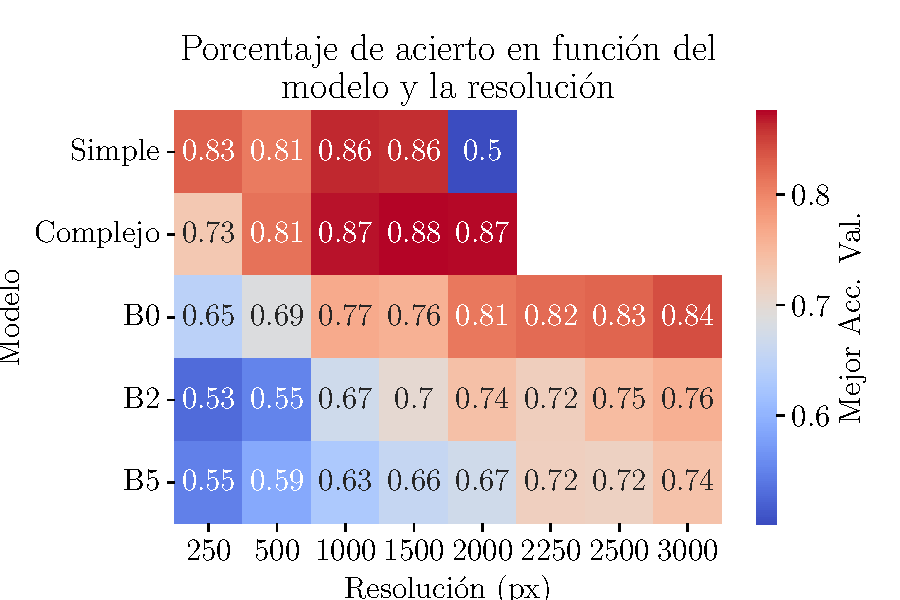
\includegraphics[scale=0.85]{tab_res.pdf}
  \caption{Porcentajes de acierto en para distintos modelos y distintas resoluciones (píxeles usados para describir el eje $x$ del detector) representado por un mapa de color.}
  \label{fig:estudio_res}
\end{figure}

\subsection{Ajuste de hiperparámetros}

Con todos los resultados observados surgen algunos aspectos importantes. Vemos que los modelos LeNet obtienen resultados superiores usando imágenes más pequeñas ($62\times 128$) mientras que para los modelos EfficientNet se obtienen siempre peores resultados incluso cuando se usa una resolución mayor.

Esto nos hace pensar que los modelos preentrenados deberían ser capaces de superar estos modelos simples, ya que tienen mayor información, resolución y son modelos más complejos por lo que deberían de ser capaces de extraer patrones más complejo. Además, al haber sido entrenados con muchas imágenes, el entrenamiento tiene que ser más simple. Los modelos LeNet se diseñaron con la idea de centrarse únicamente en el origen de la cascada al ser el punto donde teóricamente hay más diferencias y vemos que se obtienen muy buenos resultados. Teniendo todo esto en cuenta es posible que para los modelos LeNet estemos muy cerca del máximo que se puede conseguir teniendo en cuenta que estamos usando una representación desprecia una dimensión completa y que se pierde mucha información en las imágenes debido al tamaño y resolución que estamos usando.

Por todo esto, ahora vamos a ajustar los hiperparámetros de los distintos modelos centrándonos en los modelos preentrenados donde si es esperable una gran mejora ya que al menos deben de ser capaces de igualar los modelos LeNet. Para los modelos LeNet lo que haremos es ajustar algunos hiperparámetros pero no esperamos que se consigan mejoras significativas.

% Por un lado vamos a hacer modificaciones sobre los modelos LeNet modificando parámetros como el tamaño de los filtros y su desplazamiento. Además haremos pruebas para distintos ritmos de aprendizaje. Por otro lado haremos pruebas sobre los modelos preentrenados modificando el número de capas a reentrenar así como el el clasificador empleado para clasificar en función de las características aprendidas.

\subsubsection*{LeNet}
\begin{table}[h!]
  \centering
  \begin{tabular}{|cc||cc|cc|cc|cc|}
  \hline
  \multicolumn{2}{|c||}{\multirow{2}{*}{}}    & \multicolumn{1}{c|}{ks}         & kd        & \multicolumn{1}{c|}{ks}         & kd        & \multicolumn{1}{c|}{ks}         & kd        & \multicolumn{1}{c|}{ks}         & kd        \\ \cline{3-10} 
  \multicolumn{2}{|c||}{}                     & \multicolumn{1}{c|}{3}          & 1         & \multicolumn{1}{c|}{5}          & 1         & \multicolumn{1}{c|}{3}          & 2         & \multicolumn{1}{c|}{5}          & 2         \\ \hline\hline
  \multicolumn{1}{|c|}{lr}       & 10$^{-3}$ & \multicolumn{2}{c|}{\multirow{2}{*}{0.883}} & \multicolumn{2}{c|}{\multirow{2}{*}{0.891}} & \multicolumn{2}{c|}{\multirow{2}{*}{0.771}} & \multicolumn{2}{c|}{\multirow{2}{*}{0.718}} \\ \cline{1-2}
  \multicolumn{1}{|c|}{$\gamma$} & 1.0       & \multicolumn{2}{c|}{}                       & \multicolumn{2}{c|}{}                       & \multicolumn{2}{c|}{}                       & \multicolumn{2}{c|}{}                       \\ \hline
  \multicolumn{1}{|c|}{lr}       & 10$^{-3}$ & \multicolumn{2}{c|}{\multirow{2}{*}{0.884}} & \multicolumn{2}{c|}{\multirow{2}{*}{0.892}} & \multicolumn{2}{c|}{\multirow{2}{*}{0.768}} & \multicolumn{2}{c|}{\multirow{2}{*}{0.727}} \\ \cline{1-2}
  \multicolumn{1}{|c|}{$\gamma$} & 0.8       & \multicolumn{2}{c|}{}                       & \multicolumn{2}{c|}{}                       & \multicolumn{2}{c|}{}                       & \multicolumn{2}{c|}{}                       \\ \hline
  \multicolumn{1}{|c|}{lr}       & 10$^{-3}$ & \multicolumn{2}{c|}{\multirow{2}{*}{0.881}} & \multicolumn{2}{c|}{\multirow{2}{*}{0.887}} & \multicolumn{2}{c|}{\multirow{2}{*}{0.763}} & \multicolumn{2}{c|}{\multirow{2}{*}{0.728}} \\ \cline{1-2}
  \multicolumn{1}{|c|}{$\gamma$} & 0.7       & \multicolumn{2}{c|}{}                       & \multicolumn{2}{c|}{}                       & \multicolumn{2}{c|}{}                       & \multicolumn{2}{c|}{}                       \\ \hline
  \multicolumn{1}{|c|}{lr}       & 10$^{-3}$ & \multicolumn{2}{c|}{\multirow{2}{*}{0.875}} & \multicolumn{2}{c|}{\multirow{2}{*}{0.886}} & \multicolumn{2}{c|}{\multirow{2}{*}{0.762}} & \multicolumn{2}{c|}{\multirow{2}{*}{0.718}} \\ \cline{1-2}
  \multicolumn{1}{|c|}{$\gamma$} & 0.5       & \multicolumn{2}{c|}{}                       & \multicolumn{2}{c|}{}                       & \multicolumn{2}{c|}{}                       & \multicolumn{2}{c|}{}                       \\ \hline
  \multicolumn{1}{|c|}{lr}       & 10$^{-4}$ & \multicolumn{2}{c|}{\multirow{2}{*}{0.818}} & \multicolumn{2}{c|}{\multirow{2}{*}{0.862}} & \multicolumn{2}{c|}{\multirow{2}{*}{0.627}} & \multicolumn{2}{c|}{\multirow{2}{*}{0.593}} \\ \cline{1-2}
  \multicolumn{1}{|c|}{$\gamma$} & 1.0       & \multicolumn{2}{c|}{}                       & \multicolumn{2}{c|}{}                       & \multicolumn{2}{c|}{}                       & \multicolumn{2}{c|}{}                       \\ \hline
  \multicolumn{1}{|c|}{lr}       & 10$^{-4}$ & \multicolumn{2}{c|}{\multirow{2}{*}{0.758}} & \multicolumn{2}{c|}{\multirow{2}{*}{0.836}} & \multicolumn{2}{c|}{\multirow{2}{*}{0.597}} & \multicolumn{2}{c|}{\multirow{2}{*}{0.573}} \\ \cline{1-2}
  \multicolumn{1}{|c|}{$\gamma$} & 0.8       & \multicolumn{2}{c|}{}                       & \multicolumn{2}{c|}{}                       & \multicolumn{2}{c|}{}                       & \multicolumn{2}{c|}{}                       \\ \hline
  \multicolumn{1}{|c|}{lr}       & 10$^{-4}$ & \multicolumn{2}{c|}{\multirow{2}{*}{0.713}} & \multicolumn{2}{c|}{\multirow{2}{*}{0.803}} & \multicolumn{2}{c|}{\multirow{2}{*}{0.612}} & \multicolumn{2}{c|}{\multirow{2}{*}{0.584}} \\ \cline{1-2}
  \multicolumn{1}{|c|}{$\gamma$} & 0.7       & \multicolumn{2}{c|}{}                       & \multicolumn{2}{c|}{}                       & \multicolumn{2}{c|}{}                       & \multicolumn{2}{c|}{}                       \\ \hline
  \multicolumn{1}{|c|}{lr}       & 10$^{-4}$ & \multicolumn{2}{c|}{\multirow{2}{*}{0.657}} & \multicolumn{2}{c|}{\multirow{2}{*}{0.764}} & \multicolumn{2}{c|}{\multirow{2}{*}{0.609}} & \multicolumn{2}{c|}{\multirow{2}{*}{0.578}} \\ \cline{1-2}
  \multicolumn{1}{|c|}{$\gamma$} & 0.5       & \multicolumn{2}{c|}{}                       & \multicolumn{2}{c|}{}                       & \multicolumn{2}{c|}{}                       & \multicolumn{2}{c|}{}                       \\ \hline
  \end{tabular}
  \caption{Resultados de la búsqueda de rejilla realizada sobre el modelo LeNet simple. Se han modificado el ritmo de aprendizaje $lr$, la cantidad que se modifica el $lr$, el tamaño de los filtros $ks$ y su desplazamiento $ks$.}
  \label{tab:resultados_kernel_simple}
\end{table}

Como ya hemos puesto en manifiesto en varias ocasiones, tenemos una gran cantidad de parámetros y no nos podemos permitir hacer una búsqueda sobre todos ellos. Por todo esto vamos a probar a modificar 4 parámetros: el ritmo de aprendizaje ($lr$), lo que se modifica el ritmo de aprendizaje ($\gamma$), el tamaño de los filtros ($ks$) y el desplazamiento ($kd$). Las pruebas las vamos a realizar para ambos modelos y en las Tablas \ref{tab:resultados_kernel_simple} y \ref{tab:resultados_kernel_complejo} se recogen los resultados. En el Anexo se muestran los hiperparámetros en detalle.

% Please add the following required packages to your document preamble:
% \usepackage{multirow}
% Please add the following required packages to your document preamble:
% \usepackage{multirow}

% Please add the following required packages to your document preamble:
% \usepackage{multirow}
\begin{table}[h!]
  \centering
  \begin{tabular}{|cc||cc|cc|cc|cc|}
  \hline
  \multicolumn{2}{|c||}{\multirow{2}{*}{}} & \multicolumn{1}{c|}{ks} & kd & \multicolumn{1}{c|}{ks} & kd & \multicolumn{1}{c|}{ks} & kd & \multicolumn{1}{c|}{ks} & kd \\ \cline{3-10} 
  \multicolumn{2}{|c||}{}                  & \multicolumn{1}{c|}{3}  & 1  & \multicolumn{1}{c|}{5}  & 1  & \multicolumn{1}{c|}{3}  & 2  & \multicolumn{1}{c|}{5}  & 2  \\ \hline\hline
  \multicolumn{1}{|c|}{$\gamma$}   & 1.0  & \multicolumn{2}{c|}{0.875}   & \multicolumn{2}{c|}{0.857}   & \multicolumn{2}{c|}{0.516}   & \multicolumn{2}{c|}{0.858}   \\ \hline
  \multicolumn{1}{|c|}{$\gamma$}   & 0.8  & \multicolumn{2}{c|}{0.879}   & \multicolumn{2}{c|}{0.857}   & \multicolumn{2}{c|}{0.516}   & \multicolumn{2}{c|}{0.526}   \\ \hline
  \multicolumn{1}{|c|}{$\gamma$}   & 0.5  & \multicolumn{2}{c|}{0.870}   & \multicolumn{2}{c|}{0.767}   & \multicolumn{2}{c|}{0.516}   & \multicolumn{2}{c|}{0.484}   \\ \hline
  \end{tabular}
  \caption{Resultados de la búsqueda de rejilla realizada sobre el modelo  LeNet complejo. Se han modificado la cantidad que se modifica el $lr$, el tamaño de los filtros $ks$ y su desplazamiento $ks$. \red{En el anexo mostrar más detalles de los parámetros.}}
  \label{tab:resultados_kernel_complejo}
  \end{table}

La rejilla usada es muy simple donde hemos probado solo un par de valores para cada parámetro y aun así el número de pruebas realizadas al final de entorno a 50 ya que se ha realizado algunas más y descartados otras. En concreto hemos hecho 32 pruebas para el modelo simple y 15 para el complejo y la rejilla consiste en:
\begin{itemize}
  \item \inline{optim_lr} $\in \left[0.0001, 0.001\right]$.
  \item \inline{scheduler_gamma} $\in \left[0.5, 0.7, 0.8, 1\right]$.
  \item \inline{kernel_stride} $\in \left[1, 2\right]$.
  \item \inline{kernel_size} $\in \left[3, 5\right]$.
\end{itemize}

\begin{figure}[h!]
  \centering
  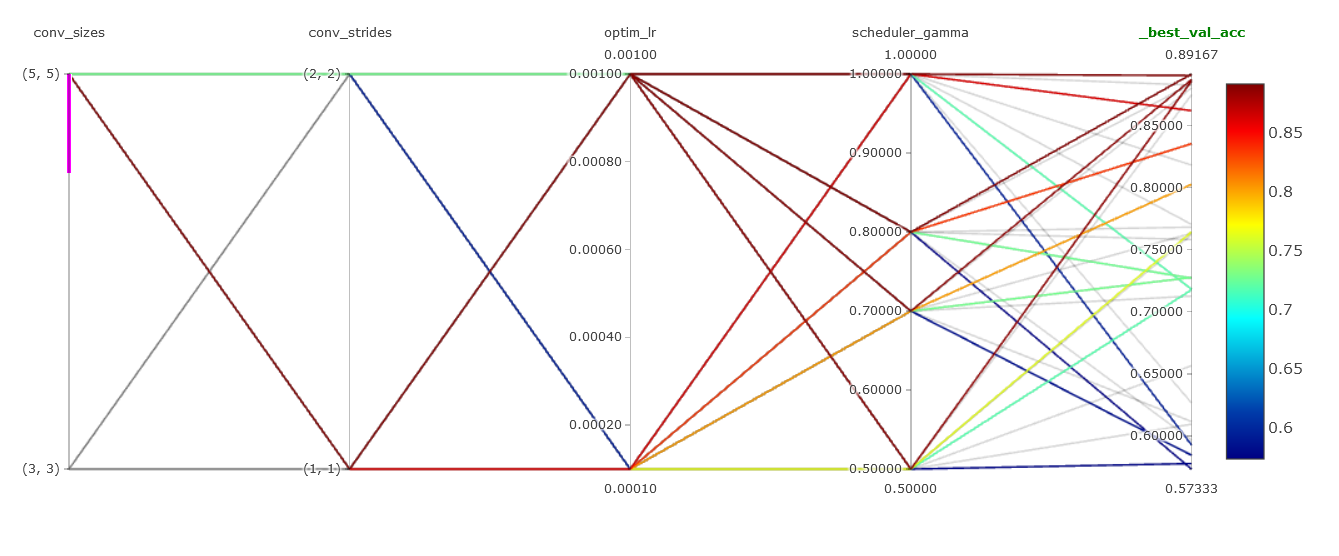
\includegraphics[scale=0.65, center]{studio_kernel_simple.PNG}
  \caption{Gráfica obtenida de MLFlow con los resultados de la búsqueda de rejilla aplicada sobre el modelo simple con una resolución de 1500 px.}
  \label{fig:estudio_kernel}
\end{figure}


Para estudiar los resultados hemos usado MLFlow que nos permite comparar experimentos y hacer gráficas mostrando los distintos hiperparámetros y los resultados de esos experimentos en la Fig. \ref{fig:estudio_kernel} muestro un ejemplo de la gráfica obtenida y además no permite seleccionar rango de los parámetros para ver que ``hilos'' estamos viendo. Las conclusiones que podemos llegar de los resultados del modelo simple son:
\begin{itemize}
  \item Siempre se observa que los resultados son peores cunado se usa un desplazamiento de los filtros de 2 px frente a usar un $kd = 1$ px.
  \item De igual manera se observa con el $lr$, donde el $lr = 0.0001$ siempre da peores resultados frente a usar $lr = 0.001$. El resto de conclusiones las vamos a limitar estos casos.
  \item También vemos que en general a medida que disminuimos el gamma del cambio de \textit{lr} dinámico vemos que los resultados empeoran pero el máximo se encuentra en 0.8 siendo ligeramente peor cuando el gamma es 1.0.
  \item Siempre se observan mejores resultados con los filtros 5 px de tamaño. 
  \item El mejor resultado se tiene con un 0.892 para $lr = 0.001$, $\gamma = 0.8$, $ks = 5$ px y $kd = 1$ px.
\end{itemize}

Para el modelo complejo:
\begin{itemize}
  \item Para este caso hemos quitado un valor de $\gamma$ y vimos que cuando se tenía $lr = 0.001$ el modelo no aprendía por lo que no hicimos todas las pruebas y no se muestran. Además hemos tenido que introducir modificar las imágenes introduciendo lo que se denomina \textit{padding} para que al aplicar los filtros no se reduzca mucho la imagen.
    \item Siempre se obtienen mejores resultados cuando el desplazamiento es de 1 px.
  \item Con respecto al $\gamma$ vemos que los mejores resultados se tienen con $\gamma = 0.8$ y parece que lo mejor es cuando es 0.8 ó 1.0.
  \item A diferencia que lo que se observaba con el modelo simple, se obtiene mejores resultados con el $ks = 3$ px
  \item El mejor resultado se tiene con un 0.879 para $lr = 0.0001$, gamma = 0.7, $ks = 3$ px y $kd = 1$ px.
\end{itemize}

En resumen, vemos que hemos tras el ajuste hemos obtenido mejores resultados con el modelo simple, usando filtros algo mayores de los que estábamos usando. El resto de parámetros es prácticamente el mismo. La mejora obtenida es de un 1\% que es considerablemente bajo teniendo en cuenta que hemos hecho más de 50 pruebas para llegar a este valor.

Por otro lado, aunque es posible que se mejoren aun más los resultados si buscamos en otros parámetros, pero para esto serían necesario realizar muchas pruebas. Previamente a este trabajo, el \red{no se que poner aquí} han abordado el mismo problema pero sin hacer uso de imágenes, usando los datos tabulares codificados de manera que se mantiene toda la información. Con este ajuste ya hemos conseguido superar el mejor resultado que se obtenía en este estudio que se obtenía con un Random Forest.

\subsubsection*{Modelos preentrenados}

Lo primero que vamos a hacer es tratar de establecer un valor de $\gamma$ y \textit{lr}. Como no podemos hacer esto para todos los modelos lo que vamos a hacer es establecer un prueba inicial con un clasificador complejo, un modelo intermedio como puede ser el EfficientNet B2 y usaremos un \textit{dropout} de 0.2. El clasificador usado consiste en una única capa oculta con 256 neuronas, se han descongelado 50 capas y se han probado 3 valores de $\gamma$ $\left[1.0, 0.8, 0.5\right]$ y con 3 valores de \textit{lr}: $\left[[0.0001, 0.001, 0.01]\right]$. Los mejores resultados se han obtenido con el $\gamma$ más bajo y el \textit{lr} más alto. Estos resultados se muestran en la Fig. \ref{fig:studio_optim} y se pueden consultar detenidamente en el Anexo.

\begin{figure}[h!]
  \centering
  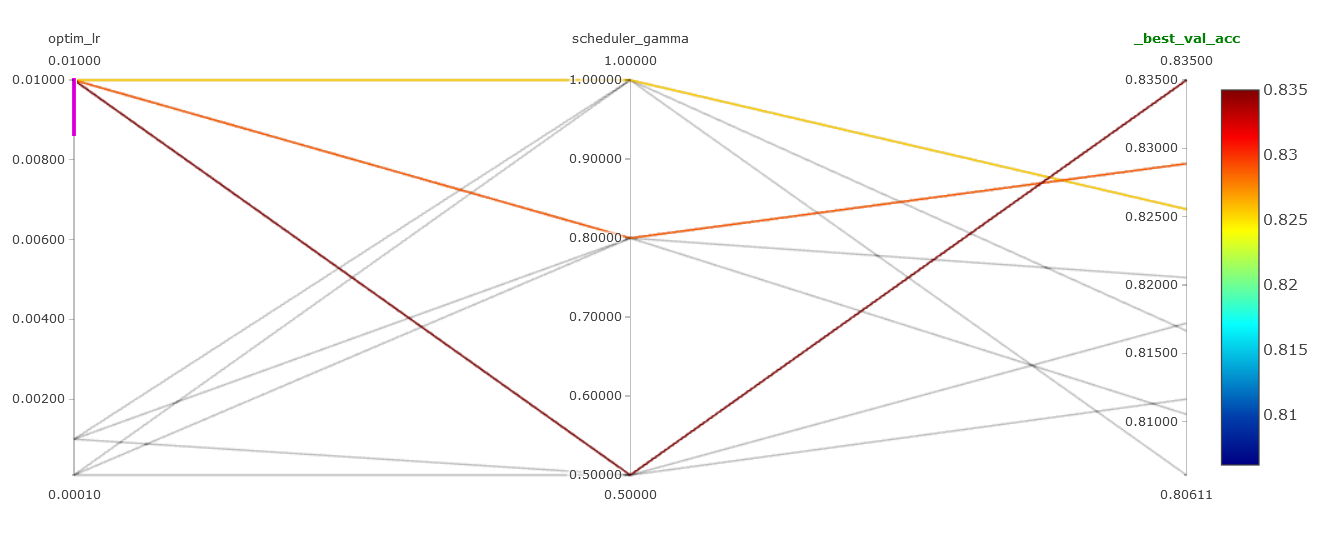
\includegraphics[scale=0.65, center]{studio_optim_pre.png}
  \caption{Gráfica obtenida de MLFlow con los resultados de la búsqueda inicial del $lr$ y de $\gamma$.}
  \label{fig:studio_optim}
\end{figure}


Con estos valores de $\gamma$ y \textit{lr} definimos una rejilla donde se modifica el clasificador y el número de capas descongeladas del extractor de características. Los clasificadores tienen una única capa oculta con 256 y 128 neuronas ($n_n$) y el número de capas a descongelar ($n_u$) probados son $\left[5, 50, 100, 300, 1000 \right]$. Hemos fijado el \textit{dropout} ($dr$) a 0.3 ya que en general hemos visto que se tiene sobre ajuste con estos modelos. Por otro lado, en algunas ocasiones las pruebas de $n_u = 1000$ no se han realizado por no tener memoria suficiente ya que los modelos que estamos usando llegan a tener muchas capas y parámetros. Hemos introducido $n_u=1000$ como caso en el que se descongelan todas las capas.  

Estas pruebas se hicieron en primer lugar usando únicamente los modelos EfficientNet B0, B2 y B5 para ver si de esta forma podíamos reducir el número de pruebas. En la Tabla \ref{tab:res_ajuste_pre} se recogen estos resultados junto con el resto de pruebas realizadas. En el Anexo se pueden consultar los detalles de los hiperparámetros.


\begin{table}[h!]
  \centering
  \begin{tabular}{|c||cc|cc|cc|c|c|}
  \hline
  \multirow{2}{*}{} & \multicolumn{2}{c|}{B0}            & \multicolumn{2}{c|}{B2}            & \multicolumn{2}{c|}{B5}             & ResNet & GoogleNet \\ \cline{2-9} 
                    & \multicolumn{1}{c|}{256}   & 128   & \multicolumn{1}{c|}{256}   & 128   & \multicolumn{1}{c|}{256}    & 128   & 256    & 256       \\ \hline\hline
  5                 & \multicolumn{1}{c|}{0.737} & 0.838 & \multicolumn{1}{c|}{0.749} & 0.756 & \multicolumn{1}{c|}{0.729}  & 0.728 & 0.779  & 0.837     \\ \hline
  50                & \multicolumn{1}{c|}{0.884} & 0.878 & \multicolumn{1}{c|}{0.826} & 0.819 & \multicolumn{1}{c|}{0.808}  & 0.811 & 0.878  & 0.869     \\ \hline
  100               & \multicolumn{1}{c|}{0.889} & 0.516 & \multicolumn{1}{c|}{0.872} & 0.870 & \multicolumn{1}{c|}{0.516}  & 0.516 & 0.516  & 0.880     \\ \hline
  300               & \multicolumn{1}{c|}{0.898} & 0.839 & \multicolumn{1}{c|}{\textbf{0.913}} & 0.904 & \multicolumn{1}{c|}{0.859*} & 0.859 & 0.569  & 0.516     \\ \hline
  1000              & \multicolumn{1}{c|}{0.898} & 0.839 & \multicolumn{1}{c|}{0.854} & 0.516 & \multicolumn{1}{c|}{---}    & ---   & 0.569  & 0.516     \\ \hline
  \end{tabular}
  \caption{Resultados de hacer una búsqueda de rejilla donde se ha modificado el número de capas a reentrenar y el clasificador para distintos modelos. La primera columna hacer referencia al número de capas descongeladas $n_u$, la primera fila al modelo y la segunda al número de neuronas del clasificador $n_n$. El asterisco significa que se ha entrenado con 15 épocas.}
  \label{tab:res_ajuste_pre}
\end{table}

Lo primero que vemos es que los resultados son muy superiores a los obtenidos sin realizar la modificación de los parámetros. Por otro lado, el mejor resultado se obtiene con el modelo B2 con $n_u = 300$ y con $n_n = 256$ obteniendo un 91.3\% de acierto en validación que es una mejora considerable a los resultados obtenidos con los los modelos LeNet.

En estos resultados vemos que para los modelos EfficientNet en general se tienen mejores resultados cuando se usa $n_n = 256$ por lo que para los otro modelos vamos a usar solo este valor. Con respecto a $n_u$ no se observa ningún patrón a simple vista. Lo que si observamos es que los resultados mejoran al aumentar este parámetros hasta que se alcanza un máximo y lo resultados empeoran. Lo que puede estar ocurriendo es que al descongelar muchas se tangan muchos parámetros de manera que el optimizador no es capaz de encontrar un mínimo. 

Por otro lado, vemos que los resultados obtenidos con los modelos B5, ResNet y GoogleNet los resultados son ligeramente inferiores a los obtenidos con otros modelos pero esto puede deberse únicamente al espacio de búsqueda establecido.

Sobre estos modelos hemos hecho algunas pruebas adicionales para ver si se conseguían mejorar un poco más los resultados, sobre todo para aquellos en los que se tiene malos resultados.

\begin{itemize}
  \item ResNet 50: Hemos probado a usar $dr = 0.4$ para $n_u = 50, 100$ obteniendo 0.883, 0.891 respectivamente. Obteniendo una mejora considerable y similar a los mejores resultados obtenidos con el resto de modelos.
  \item GoogleNet: También hemos probado a usar el $dr = 0.4$ para $n_u = 100, 300$ obteniendo 0.892 y 0.516. Donde vemos que para $n_u = 100$ hemos mejorado el porcentaje de acierto llegando también a igualar al resto de modelos. Para $n_n=256$ hemos probado a usar $n_n = 128$ obteniendo 0.808. Aunque hemos conseguido mejorar los estamos lejos del resto de valores.
  \item B5: Hemos usado $n_n = 512$ para el caso que peores resultados tenía obteniendo 0.819.
  \item B0: Hemos probado a introducir $dr = 0.4$ para los mejores resultados pero se han empeorado los resultados.
\end{itemize}

A modo de conclusión de las pruebas que hemos realizado, vemos que la mayoría de  modelos llegan a superar el 0.89, de hecho, solo el B5 no lo ha conseguido. Por otro lado vemos que el B0 y B2 son los que mejores resultados han dado sobre todo el B2 que supera en un 2-3\% al resto de modelos. En general vemos que las diferencias entre los modelos no es muy alta por lo que puede que realmente la diferencia se encuentre en los parámetros siendo todos los modelos más o menos similar. Esto es algo coherente con las imágenes que estamos usando, donde puede ser complejo determinar el origen de la cascada pero los patrones que los diferencian no son complejos.

Como ya hemos repetido varias veces, no podemos afirmar que este sea el mejor modelo ya que no hemos hecho suficientes pruebas y puede que ajustar más algunos parámetros no hagan que los otros modelo lo igualen o incluso lo superen. Sin embargo, el número de necesario para esto es muy alto y con estas pocas pruebas hemos conseguido conseguido unos resultados muy buenos. En este punto es más interesante modificar las arquitecturas con la idea de tratar de recoger la información que estamos perdiendo al realizar la proyección o al fijar la ventana que seguir con la búsqueda de hiperparámetros. Para estas modificaciones haremos uso del modelo B2 al ser el que mejores resultados nos ha dado y en caso de tener problemas por la complejidad del modelo usaremos el modelo LeNet simple.

\subsection{Breve estudio del modelo B2 WIP}

Antes de hacer las modificaciones sobre la arquitectura vamos tratar hacer un breve estudio de el modelo obtenido. Recordemos que estos modelos son cajas negras cuya interpretabilidad es nula. En esta sección vamos a ver algunas métricas que nos digan como de bueno es el modelo, veremos las imágenes en las que el modelo se esta equivocando y probaremos a usar una técnica que nos permita visualizar las regiones de la imagen que más influyen en la decisión. Además obtendremos la eficiencia y pureza del modelo en función de la energía y veremos como se re modifican los resultados si quitamos \textit{hits} de la imagen.

\subsection{Concatenación de redes, 3 proyecciones WIP}

Hasta ahora hemos usado únicamente una de las proyecciones para realizar la clasificación. En esta sección vamos a tratar de mejorar los resultados juntando las tres redes usando ensembles y

% \subsection{Concatenación de redes, varias regiones.}

% Al igual que estamos perdiendo información al realizar la proyección, se pierde información al establecer la ventana perdiendo información del final de la cascada. Nuestro objetivo es probar a entrenar un modelo con la parte inicial y otro con la final y agregar esta información para tratar de mejora los resultados.

% \subsection{Visual Transformers WIP}

% A lo largo del trabajo hemos hecho mención de los Tranformers y que han mostrado buenos resultados para distintos problemas. En esta sección queremos hacer una prueba de concepto del funcionamiento de este modelo sobre las imágenes para ver si obtienen mejores resultados.

\section{Conclusiones y trabajos futuros}

TODO
\begin{itemize}
  \item estudio modelo
  % \item ViT
  \item Concatenación proyecciones
  % \item Concatenación de regiones
  \item Anexo de código
  \item Anexo hiperparámetros
  \item Abstract
  \item Conclusiones
  \item Arreglar una cosa de MLFlow
\end{itemize}

\newpage

\printbibliography[title={Bibliografía}]



\end{document}